% ===================================================================
%  Chronos-ESM: A Differentiable Earth System Model
%  Manual & Textbook  —  build with:  latexmk -pdf main.tex
% ===================================================================
\documentclass[11pt,openany]{book}
% ===================================================================
% Chronos-ESM Manual — shared preamble (packages, notation, styles)
% ===================================================================
\usepackage[utf8]{inputenc}
\usepackage[T1]{fontenc}
\usepackage{lmodern}
\usepackage[a4paper,margin=1in]{geometry}
\usepackage{amsmath,amssymb,amsthm,mathtools}
\usepackage{bm}
\usepackage{graphicx}
\graphicspath{{figures/}{../figures/}}   % manual figures and the repo docs/figures
\usepackage{booktabs}
\usepackage{array}
\usepackage{xcolor}
\usepackage{listings}
\usepackage[round]{natbib}
\usepackage[colorlinks=true,linkcolor=NavyBlue,citecolor=ForestGreen,urlcolor=BrickRed]{hyperref}
\usepackage{caption}
\usepackage{microtype}
\usepackage{enumitem}

% --- colours -------------------------------------------------------
\definecolor{NavyBlue}{RGB}{0,51,153}
\definecolor{ForestGreen}{RGB}{34,102,51}
\definecolor{BrickRed}{RGB}{153,0,0}
\definecolor{codebg}{RGB}{245,245,248}
\definecolor{codekw}{RGB}{0,0,153}
\definecolor{codecomment}{RGB}{102,102,102}
\definecolor{codestr}{RGB}{153,51,0}

% --- Python code listings (map equations <-> implementation) -------
\lstdefinestyle{chronos}{
  language=Python, backgroundcolor=\color{codebg},
  basicstyle=\ttfamily\footnotesize, keywordstyle=\color{codekw}\bfseries,
  commentstyle=\color{codecomment}\itshape, stringstyle=\color{codestr},
  showstringspaces=false, breaklines=true, frame=single, framerule=0pt,
  numbers=left, numberstyle=\tiny\color{codecomment}, captionpos=b, tabsize=4,
}
\lstset{style=chronos}

% --- theorem-like environments -------------------------------------
\theoremstyle{definition}
\newtheorem{exercise}{Exercise}[chapter]
\newtheorem{example}{Example}[chapter]
\theoremstyle{remark}
\newtheorem*{remark}{Remark}
\theoremstyle{plain}
\newtheorem{proposition}{Proposition}[chapter]

% "Code box": a marginless callout mapping math to a source location
\newcommand{\codref}[2]{\par\noindent\textcolor{ForestGreen}{\small$\hookrightarrow$ \textit{Code:} \texttt{#1} — #2}\par}

% ===================================================================
% NOTATION MACROS — chapter authors MUST use these for consistency.
% ===================================================================
% calculus
\newcommand{\pd}[2]{\frac{\partial #1}{\partial #2}}        % partial derivative
\newcommand{\pdd}[2]{\frac{\partial^2 #1}{\partial #2^2}}
\newcommand{\dt}[1]{\frac{\mathrm{d}#1}{\mathrm{d}t}}
\newcommand{\Dt}[1]{\frac{\mathrm{D}#1}{\mathrm{D}t}}        % material derivative
\newcommand{\grad}{\boldsymbol{\nabla}}
\newcommand{\diver}{\grad\!\cdot\!}
\newcommand{\curl}{\grad\!\times\!}
\newcommand{\lap}{\nabla^{2}}
\newcommand{\dd}{\,\mathrm{d}}
% vectors / fields
\newcommand{\uvec}{\mathbf{u}}                 % horizontal velocity vector
\newcommand{\kvec}{\mathbf{k}}                 % vertical unit vector
\newcommand{\xvec}{\mathbf{x}}
\newcommand{\uu}{u}                            % zonal velocity
\newcommand{\vv}{v}                            % meridional velocity
\newcommand{\ww}{w}                            % vertical velocity
\newcommand{\Temp}{\theta}                     % potential temperature
\newcommand{\Salt}{S}                          % salinity
\newcommand{\dens}{\rho}                       % density
\newcommand{\densz}{\rho_0}                    % reference density
\newcommand{\pres}{p}                          % pressure
\newcommand{\psib}{\psi}                       % streamfunction
\newcommand{\vort}{\zeta}                      % relative vorticity
% parameters / constants
\newcommand{\Cor}{f}                           % Coriolis parameter
\newcommand{\beq}{\beta}                       % beta = df/dy
\newcommand{\Erad}{a}                          % Earth radius
\newcommand{\Om}{\Omega}                       % Earth rotation rate
\newcommand{\grav}{g}                          % gravity
\newcommand{\lat}{\phi}                        % latitude
\newcommand{\lon}{\lambda}                     % longitude
\newcommand{\dep}{H}                           % ocean depth / column thickness
% software / discrete
\newcommand{\code}[1]{\texttt{#1}}
\newcommand{\jax}{\textsc{jax}}
\newcommand{\dino}{\textsc{dinosaur}}
\newcommand{\model}{Chronos-ESM}
\newcommand{\softplus}{\operatorname{softplus}}
\newcommand{\Sv}{\,\mathrm{Sv}}                % Sverdrup


\title{\bfseries Chronos-ESM\\[0.3em]\large A Differentiable Earth System Model\\[0.6em]
       \normalsize Theory, Numerics, and Climate Applications}
\author{Bijan Fallah \\ \small and the Chronos-ESM contributors}
\date{Compiled \today}

\begin{document}
\frontmatter
\maketitle

\thispagestyle{empty}
\vspace*{\fill}
\noindent\small
Copyright \textcopyright{} 2026 Bijan Fallah and the Chronos-ESM contributors.\\
This manual accompanies the Chronos-ESM source code (Apache License 2.0) and is intended
for research and teaching. It is a living document, generated alongside the code so that
every governing equation is traceable to its implementation.\\[1em]
Source: \url{https://github.com/bijanf/ESMB}
\vspace*{\fill}
\clearpage

\chapter*{Preface}
\addcontentsline{toc}{chapter}{Preface}

\model{} is a fully \emph{differentiable}, GPU- and CPU-capable coupled Earth System Model
written in \jax{}. It couples a multi-level spectral primitive-equation atmosphere (built on
Google's \dino{} dynamical core), a $z$-level primitive-equation ocean, a thermodynamic sea
ice model, and a land-surface scheme, at a teaching-friendly T31 ($\approx 3.75^\circ$)
resolution that runs in minutes-to-hours on a single GPU.

This book has three aims. First, to be \textbf{equation-complete and honest}: every
prognostic equation, closure, and numerical scheme is derived from, and cross-referenced to,
the actual source code --- including its approximations and known biases. Climate-model
documentation too often hides the gap between the textbook equations and what the code really
integrates; here the two are presented together, with the code location given beside each
equation. Second, to be \textbf{pedagogical}: the model is small and fast enough that a
student can run a coupled climate experiment, change an equation, and see the result the same
afternoon. Each chapter ends with exercises that use the model as a laboratory. Third, to
showcase \textbf{differentiable Earth-system modeling}: because the entire model is written
in \jax{}, one can take the gradient of any output (global temperature, AMOC strength, a
tipping threshold) with respect to any input or parameter --- enabling calibration,
sensitivity analysis, and data assimilation that are impractical with conventional models.

The book is organized in five parts: \emph{Foundations} (the continuous and discrete
mathematics, and the differentiable-programming paradigm); \emph{The Component Models}
(ocean, atmosphere, ice, land, and the coupler, each derived from the code); \emph{Forcing,
Sensitivity, and Data Assimilation}; \emph{Canonical Climate Test Cases} (the standard
phenomena every climate model must reproduce --- mean climatology, the AMOC and its tipping,
mid-latitude jets and storm tracks, the ITCZ and monsoons); and \emph{Community, Standards,
and Teaching}, including a roadmap toward CMIP7 participation and a guide to using \model{} in
the classroom.

\bigskip
\noindent\textit{A note on status.} \model{} is research software under active development.
Where a component is a deliberate simplification or a work in progress, this book says so
explicitly --- the honest documentation of an evolving model is part of its scientific value.

\tableofcontents
\listoffigures

\mainmatter

\part{Foundations}
\chapter{Introduction: A Differentiable Earth System Model}
\label{chap:ch01_introduction}

\section{What is Chronos-ESM?}

\model{} is a coupled Earth System Model (ESM): a numerical representation of the physical
climate system in which an \emph{atmosphere}, an \emph{ocean}, \emph{sea ice}, and a
\emph{land surface} evolve together, exchanging heat, water, and momentum. What distinguishes
it from the large community models (CESM, MPI-ESM, IPSL-CM, and the rest of the CMIP fleet)
is not the physics it contains but \emph{how it is written} and \emph{how fast it runs}:

\begin{itemize}[leftmargin=1.4em]
  \item \textbf{It is differentiable.} The entire model --- every flux, every time step, every
    spectral transform --- is written in \jax{} \citep{jax2018}, a system for composable
    program transformations. As a consequence one can compute the exact gradient of \emph{any}
    scalar diagnostic (global-mean temperature, the strength of the Atlantic overturning, the
    freshwater flux at which that overturning collapses) with respect to \emph{any} input or
    tunable parameter, by automatic differentiation. This turns calibration, sensitivity
    analysis, and variational data assimilation from heroic, model-specific efforts into
    one-line operations (Part~III).
  \item \textbf{It runs on a laptop or a GPU.} At its default T31 spectral resolution
    ($\approx 3.75^\circ$, roughly $96\times48$ horizontal grid points) a coupled century
    integrates in minutes-to-hours on a single GPU, and runs --- more slowly but identically
    --- on a CPU. There is no MPI and no bespoke build system: \code{pip install} and run.
  \item \textbf{It is small enough to understand.} The whole model is about $8{,}000$ lines of
    Python. A student can read the ocean's tracer-advection routine, change the equation of
    state, and watch the climate respond the same afternoon.
\end{itemize}

These three properties --- differentiable, fast, legible --- are what make \model{} suitable
both as a research instrument for the emerging field of differentiable Earth-system science
and as a teaching model for graduate climate courses. This book serves both audiences.

\section{The model at a glance}

\model{} couples four components on a sphere of radius $\Erad$ rotating at rate $\Om$:

\begin{description}[leftmargin=0pt,style=nextline]
  \item[Atmosphere] A multi-level spectral primitive-equation dynamical core built on Google's
    differentiable \dino{} dycore --- the dynamical engine behind NeuralGCM
    \citep{kochkov2024neuralgcm}. It supports genuine baroclinic instability (growing synoptic
    eddies, a mid-latitude jet) and carries moisture for a tropical rain band. A legacy
    single-level spectral model is also provided for the cheapest experiments
    (Chapters~\ref{chap:ch09_atmosphere_multilevel}--\ref{chap:ch10_atmosphere_singlelevel}).
  \item[Ocean] A $z$-level, hydrostatic, Boussinesq primitive-equation ocean with
    Gent--McWilliams eddy transport \citep{gentmcwilliams1990}, initialized from the World
    Ocean Atlas climatology (Chapters~\ref{chap:ch04_ocean_equations}--\ref{chap:ch08_ocean_overturning}).
  \item[Sea ice] A Semtner-style thermodynamic ice model \citep{semtner1976}
    (Chapter~\ref{chap:ch11_seaice}).
  \item[Land] A slab/bucket land-surface scheme with runoff routing
    (Chapter~\ref{chap:ch12_land}).
\end{description}

The components exchange fluxes through a coupler (Chapter~\ref{chap:ch13_coupler_fluxes}) using
bulk aerodynamic formulae, with an optional flux correction that allows the coupled system to
be run either as a tightly observationally-constrained \emph{control} or as a freely-evolving,
forcing-responsive model.

\section{Philosophy: equations and code, side by side}

A recurring frustration in climate science is the distance between the equations a model is
\emph{said} to solve and the equations its code \emph{actually} integrates --- the
discretizations, the limiters, the clamps, the approximations adopted for stability. This book
takes the unusual stance that those details \emph{are} the model and deserve first-class
documentation. Throughout, each governing equation is presented in its continuous form, then in
the discrete form the code uses, with a pointer to the exact source location:

\codref{chronos\_esm/ocean/veros\_driver.py}{the ocean time step \code{step\_ocean}}

\noindent
Where a scheme is a deliberate simplification --- the single-level atmosphere's lack of vertical
structure, or the interim thermohaline closure that stands in for a prognostic overturning until
the momentum core is wired in --- we say so plainly and quantify the consequence. Honest
documentation of an evolving model is itself a scientific contribution.

\section{Why differentiability matters}

Conventional ESMs are evaluated and tuned by running them many times and comparing outputs ---
an expensive, derivative-free search over a high-dimensional parameter space. Because \model{}
is differentiable, the sensitivity of any diagnostic $J$ to any parameter vector
$\boldsymbol{\theta}$ is available directly as $\partial J/\partial\boldsymbol{\theta}$ at the
cost of roughly one extra model evaluation, by reverse-mode automatic differentiation. This
enables:
\begin{itemize}[leftmargin=1.4em]
  \item \emph{gradient-based calibration} --- fit parameters to observations by descent rather
    than by grid search;
  \item \emph{variational data assimilation} (4D-Var) --- find the initial state that best fits
    a window of observations;
  \item \emph{rigorous sensitivity and tipping analysis} --- e.g.\ locating a bifurcation by
    differentiating through the steady-state condition rather than by brute-force sweeps
    (Chapters~\ref{chap:ch15_differentiable_applications} and~\ref{chap:ch17_amoc_tipping}).
\end{itemize}
A theme of Part~III is that differentiability is powerful but not free: some targets --- notably
bifurcations such as an AMOC collapse --- are non-smooth, and require the right formulation
(fold continuation) rather than naive backpropagation through a long integration.

\section{How to read this book}

Part~I develops the continuous and discrete mathematics common to all components, and the
differentiable-programming paradigm. Part~II documents each component model in
equation-complete detail, derived from the code. Part~III covers forcing, sensitivity, and data
assimilation. Part~IV evaluates the model against the canonical phenomena every climate model
must reproduce. Part~V looks outward: a roadmap toward CMIP7 participation, and a guide to using
\model{} in the classroom. Appendices collect the notation, the parameter values, a map from
code modules to chapters, and installation instructions.

Readers wanting a fast orientation may read this chapter, then jump to the test cases of
Part~IV to see what the model produces, returning to Part~II for the mechanisms. Instructors
will find a suggested course outline in Chapter~\ref{chap:ch21_teaching}.

\begin{exercise}
Install \model{} (Appendix~\ref{chap:appD_running}) and run the shortest coupled integration in
the repository. Plot the global-mean surface temperature over the run. How long did it take, and
on what hardware?
\end{exercise}

\begin{exercise}
List three scientific questions you could ask with a differentiable climate model that would be
impractical with a conventional one. For each, identify the scalar diagnostic $J$ and the
parameter $\boldsymbol{\theta}$ whose gradient $\partial J/\partial\boldsymbol{\theta}$ you would
compute.
\end{exercise}

\chapter{Mathematical and Numerical Preliminaries}\label{chap:ch02_preliminaries}

% --- local symbols (minimal; not in the shared preamble) -------------------
\providecommand{\Cou}{C}        % Courant number
\providecommand{\nlat}{N_\lat}  % number of latitude rows
\providecommand{\nlon}{N_\lon}  % number of longitude columns

This chapter assembles the mathematical scaffolding the rest of the book stands on: the
spherical geometry every component shares, the discrete grids on which the continuous fields
live, the metric factors that the curvature of the sphere forces into every gradient and
divergence, the distinction between \emph{prognostic} variables (which the model time-steps) and
\emph{diagnostic} ones (which it reconstructs each step), and the family of time-integration
schemes the code actually uses --- with their stability limits stated honestly. Wherever a
quantity appears in the source it is pinned to its location with a code reference. The notation
fixed here is used unchanged throughout Parts~II--V.

\section{Spherical coordinates and the metric}

\model{} lives on a sphere of radius $\Erad$ (\code{EARTH\_RADIUS} $=6.371\times10^{6}\,\mathrm{m}$)
rotating at rate $\Om$ (\code{OMEGA} $=7.2921\times10^{-5}\,\mathrm{rad\,s^{-1}}$). A point is
addressed by longitude $\lon\in[0,2\pi)$, latitude $\lat\in[-\pi/2,\pi/2]$, and a vertical
coordinate (geometric depth $z$ in the ocean, a terrain-following $\sigma$ coordinate in the
multi-level atmosphere). The horizontal velocity is $\uvec=(\uu,\vv)$, with $\uu$ eastward and
$\vv$ northward, and $\ww$ is the vertical component.

\codref{chronos\_esm/config.py}{physical constants $\Erad,\Om,\grav$ and grid sizes}

The essential complication of a sphere is that the zonal arc length shrinks toward the poles.
An eastward displacement $\dd\lon$ subtends a physical distance $\Erad\cos\lat\,\dd\lon$, whereas
a northward displacement $\dd\lat$ always subtends $\Erad\,\dd\lat$. The line element is
\begin{equation}
  \dd s^2 = \Erad^2\cos^2\!\lat\;\dd\lon^2 \;+\; \Erad^2\,\dd\lat^2 \;+\; \dd z^2 .
  \label{eq:line-element}
\end{equation}
Every horizontal differential operator inherits the $\cos\lat$ factor from
\eqref{eq:line-element}. For a scalar $f$ and horizontal vector $\uvec$,
\begin{align}
  \grad f &= \left(\frac{1}{\Erad\cos\lat}\pd{f}{\lon},\;\frac{1}{\Erad}\pd{f}{\lat}\right),
  \label{eq:sph-grad}\\
  \diver\uvec &= \frac{1}{\Erad\cos\lat}\left[\pd{\uu}{\lon}
     + \pd{(\vv\cos\lat)}{\lat}\right],
  \label{eq:sph-div}\\
  \lap f &= \frac{1}{\Erad^2\cos^2\!\lat}\pdd{f}{\lon}
     + \frac{1}{\Erad^2\cos\lat}\pd{}{\lat}\!\left(\cos\lat\,\pd{f}{\lat}\right).
  \label{eq:sph-lap}
\end{align}
The $\cos\lat$ in the denominators is the source of the polar singularity that haunts every
latitude--longitude model: as $\lat\to\pm\pi/2$, a fixed zonal grid increment maps to a vanishing
physical distance, so $\partial/\partial\lon$ and $\partial^2/\partial\lon^2$ amplify any
small-scale zonal structure without bound. Section~\ref{sec:metric-discrete} shows exactly how
the two grids of \model{} cope --- one by capping the metric, the other by working in a basis in
which the singularity never appears.

The planetary rotation enters through the Coriolis parameter
\begin{equation}
  \Cor = 2\Om\sin\lat, \qquad \beq \equiv \pd{\Cor}{y} = \frac{2\Om\cos\lat}{\Erad},
  \label{eq:coriolis}
\end{equation}
the second of which is the $\beta$ that controls Rossby propagation and the western
intensification of ocean gyres. In the ocean driver $\Cor$ is built directly from a uniform
latitude vector, \code{f\_cor = 2*OMEGA*sin(lat\_rad)}, and is floored away from zero near the
equator (to $|\Cor|\ge 10^{-5}\,\mathrm{s^{-1}}$) so that the geostrophic/Stommel division by
$\Cor$ stays finite there.

\codref{chronos\_esm/ocean/veros\_driver.py}{$\Cor$ from latitude, equatorial floor in \code{step\_ocean}}

\section{The model grids}

\model{} runs at spectral truncation \textbf{T31} by default, an option set by the environment
variable \code{CHRONOS\_RESOLUTION} (\code{T31} or \code{T63}). At T31 the horizontal grid is
$\nlon\times\nlat = 96\times48$, i.e.\ a nominal $3.75^\circ$ spacing.

\codref{chronos\_esm/config.py}{\code{RESOLUTION}, \code{NLAT=48}, \code{NLON=96}}

\subsection{The ocean grid: latitude--longitude, $z$-level}

The ocean is discretized on a regular latitude--longitude mesh with $96$ cells in longitude and
$48$ in latitude, the row centres laid out by \code{linspace(-90, 90, ny)}. Longitude spacing is
uniform, $\Delta\lon = 2\pi/\nlon$; the corresponding physical zonal spacing is latitude
dependent,
\begin{equation}
  \Delta x(\lat) = \Erad\cos\lat\,\Delta\lon, \qquad
  \Delta y = \frac{\pi\,\Erad}{\nlat}\;\;(\text{uniform}),
  \label{eq:ocean-dxdy}
\end{equation}
exactly the metric of \eqref{eq:line-element}. The driver receives $\Delta x$ as an array (it
varies down the column) and $\Delta y$ as a scalar.

Vertically the ocean carries $N_z=15$ levels on a \emph{stretched} grid, not a uniform one. A
uniform $5000/15\approx 333\,\mathrm{m}$ surface layer would give the sea surface an enormous
heat capacity and a sluggish response to fluxes, because surface forcing is applied as
$\text{flux}/(\dens_0 c_p\,\Delta z_0)$. Instead the interfaces are placed at
\begin{equation}
  z_i = \dep_{\mathrm{tot}}\left(\frac{i}{N_z}\right)^{\!s}, \quad i=0,\dots,N_z,\qquad
  \dep_{\mathrm{tot}}=5000\,\mathrm{m},\;\; s=1.7,
  \label{eq:ocean-vgrid}
\end{equation}
so that $\Delta z_k = z_{k+1}-z_k$ grows from a thin ($\approx 50\,\mathrm{m}$) surface layer to
a thick abyssal one, with layer-centre depths $\tfrac12(z_k+z_{k+1})$ used as the coordinate onto
which the World Ocean Atlas initial state is interpolated.

\codref{chronos\_esm/config.py}{\code{\_ocean\_vertical\_grid}, \code{OCEAN\_DZ}, \code{OCEAN\_DEPTH\_CENTERS}}

\begin{remark}
The ocean driver computes horizontal derivatives with plain centred differences of the form
$(\code{roll}(F,-1)-\code{roll}(F,1))/(2\Delta x)$ and treats $\Delta x,\Delta y$ as local
Cartesian spacings; the spherical \emph{convergence-of-meridians} term in the divergence,
$\partial(\vv\cos\lat)/\partial\lat$ of \eqref{eq:sph-div}, is approximated by the Cartesian
$\partial\vv/\partial\lat$ (no explicit $\cos\lat$ metric in the meridional divergence). This is a
known simplification; the diagnostic vertical velocity comment in the source flags it explicitly.
It is acceptable at this resolution but is one of the contributors to the spurious net meridional
transport that the per-latitude corrector of Chapter~\ref{chap:ch08_ocean_overturning} removes.
\end{remark}

\subsection{The atmosphere grids: spectral on a Gaussian mesh}

The atmosphere is \emph{spectral}: prognostic fields are represented not by their grid-point
values but by coefficients in a basis of spherical harmonics $Y_l^m(\lat,\lon)$, and the
``T31'' label is the triangular truncation total wavenumber $l\le 31$. Two atmospheres coexist
in the code.

\paragraph{Single-level (legacy).} The barotropic model in
\code{atmos/dynamics.py} is a hybrid pseudo-spectral scheme: it takes the FFT in longitude (exact
for the periodic direction) and uses fourth-order finite differences in latitude. Its grid is the
same regular $96\times48$ latitude--longitude mesh as the ocean, with the metric of
\eqref{eq:ocean-dxdy}.

\codref{chronos\_esm/atmos/spectral.py}{\code{compute\_gradients} --- FFT in $\lon$, 4th-order FD in $\lat$}

\paragraph{Multi-level (active).} The production atmosphere is Google's differentiable \dino{}
dycore (the engine behind NeuralGCM, \citealp{kochkov2024neuralgcm}), run at T31 with $24$
$\sigma$-levels and full spherical-harmonic transforms. Its horizontal grid is a \emph{Gaussian}
mesh: the latitude rows sit at the roots of the Legendre polynomial $P_{\nlat}(\sin\lat)$, chosen
so that Gauss--Legendre quadrature integrates the truncated harmonics exactly. Grid$\to$spectral
and spectral$\to$grid maps are \code{coords.horizontal.to\_modal} /
\code{to\_nodal}, and the eastward/northward winds are recovered from the modal state as
\begin{equation}
  \uu = \frac{(\widehat{\uu\cos\lat})_{\,0}}{\cos\lat}, \qquad
  \vv = \frac{(\widehat{\uu\cos\lat})_{\,1}}{\cos\lat},
  \label{eq:dino-uv}
\end{equation}
i.e.\ the dycore carries the momentum-like quantity $\uvec\cos\lat$ (regular at the poles) and
divides out $\cos\lat$ only for diagnostics --- the spectral route never divides by $\cos\lat$
internally, which is precisely why it has no polar instability.

\codref{chronos\_esm/atmos/dino\_atmos.py}{T31, $24$ $\sigma$-levels; \code{compute\_diagnostic\_state} for $\uu,\vv$}

\subsection{Metric terms in the discrete code}\label{sec:metric-discrete}

The single-level model must build the metric by hand. It forms the per-row zonal spacing
$\Delta x(\lat)=2\pi\Erad\cos\lat/\nlon$ and $\Delta y=\pi\Erad/\nlat$ directly. The polar
catastrophe implicit in the $1/\cos\lat$ factors of \eqref{eq:sph-grad}--\eqref{eq:sph-lap} is
dealt with by a hard floor on the cosine used in the \emph{dynamics}: rather than letting $\Delta x\to 0$ (it reaches $\approx 4\,\mathrm{m}$ in
the polar row when $\cos\lat$ is floored to $10^{-5}$), the metric is capped at its $80^\circ$
value,
\begin{equation}
  \cos\lat\big|_{\mathrm{dyn}} = \max\!\big(\cos\lat,\;\cos 80^\circ\big),
  \qquad \Delta x = \frac{2\pi\Erad\,\cos\lat\big|_{\mathrm{dyn}}}{\nlon},
  \label{eq:cos-floor}
\end{equation}
so the handful of pole-most rows integrate with the (still small) $80^\circ$ metric instead of
detonating. A separate, slightly different floor is applied to the diffusion $\Delta x$ so the
explicit hyperdiffusion stencil $\propto 1/\Delta x^4$ stays inside its stability bound. This is a
pragmatic fix, not a clean discretization: without it the mean sea-level pressure blew up at the
poles to $\sigma\sim 150\,\mathrm{hPa}$ against an observed $\sim 12\,\mathrm{hPa}$. The \dino{}
atmosphere needs no such floor because, as in \eqref{eq:dino-uv}, the singular $1/\cos\lat$ is
never formed.

\codref{chronos\_esm/atmos/dynamics.py}{\code{cos\_lat\_dyn}/\code{cos\_lat\_diff} floors in \code{step\_atmos}}

\section{Prognostic and diagnostic variables}\label{sec:prog-diag}

A central organizing idea is the split between \textbf{prognostic} variables --- those that carry
a time derivative and are advanced by the integrator --- and \textbf{diagnostic} variables ---
those reconstructed each step from the prognostic state by solving a (usually elliptic) balance.
The split is not cosmetic: it is what makes a step well-posed, and it determines what must be
saved in a checkpoint to restart bit-for-bit.

In the ocean, the \code{OceanState} carries eight fields, but only the three tracers are truly
prognostic in the time-stepping sense. Temperature $\Temp$, salinity $\Salt$, and dissolved
inorganic carbon are advanced by an explicit Runge--Kutta step (Section~\ref{sec:time}); density,
the velocities $(\uu,\vv,\ww)$, and the barotropic streamfunction $\psib$ are \emph{diagnosed}
each step from the tracers via the equation of state, thermal wind, continuity, and a Stommel
balance respectively. Table~\ref{tab:prog-diag} summarizes the split.

\codref{chronos\_esm/ocean/veros\_driver.py}{\code{OceanState}; tracers stepped, $\uvec,\ww,\dens,\psib$ diagnosed}

\begin{table}[ht]
\centering
\caption{Prognostic vs.\ diagnostic variables in the ocean and the active atmosphere.}
\label{tab:prog-diag}
\begin{tabular}{@{}lll@{}}
\toprule
Component & Prognostic (time-stepped) & Diagnostic (reconstructed) \\
\midrule
Ocean & $\Temp,\;\Salt,\;\text{DIC}$ & $\dens,\;\uu,\;\vv,\;\ww,\;\psib$ \\
Atmosphere (\dino) & $\vort,\;\delta,\;T',\;\ln p_s$, humidity & $\uu,\vv$ (from \eqref{eq:dino-uv}), $\Temp$, geopotential \\
\bottomrule
\end{tabular}
\end{table}

The diagnostic velocities follow from the linear equation of state
\begin{equation}
  \dens = \densz - \alpha(\Temp-\Temp_0) + \beta(\Salt-\Salt_0),
  \quad \densz=1025,\;\alpha=0.2,\;\beta=0.8,
  \label{eq:eos}
\end{equation}
followed by a thermal-wind/geostrophic relation for the baroclinic shear and a Stommel
streamfunction for the barotropic flow; these are derived in
Chapters~\ref{chap:ch04_ocean_equations} and~\ref{chap:ch06_ocean_numerics}. Because the
velocities are diagnostic, a restart need only store the tracers (plus $\psib$ as a warm start for
the elliptic solve); the rest is rebuilt on the first step. The same logic governs \dino{}
checkpoints, whose prognostic modal state is vorticity $\vort$, divergence $\delta$, temperature
variation $T'$, and log surface pressure $\ln p_s$; $\uu,\vv$ are diagnostic. (A subtle
consequence: restoring \code{sim\_time=None} on resume is mandatory, because the ImEx integrator
adds a tendency \emph{array} to the clock and a stored scalar would break that add.)

\codref{chronos\_esm/ocean/veros\_driver.py}{\code{equation\_of\_state} --- linear EOS, $\alpha,\beta$}

\section{Time-integration schemes}\label{sec:time}

\model{} uses different time integrators in different components, each chosen for the stiffness
and conservation demands of the equations it solves. We state each in the canonical
$\dt{\boldsymbol\Phi}=\mathcal{R}(\boldsymbol\Phi)$ form, where $\boldsymbol\Phi$ is the
prognostic state and $\mathcal{R}$ its tendency.

\subsection{Forward Euler --- the single-level atmosphere}

The legacy barotropic atmosphere advances with the simplest possible scheme,
\begin{equation}
  \boldsymbol\Phi^{n+1} = \boldsymbol\Phi^{n} + \Delta t\,\mathcal{R}(\boldsymbol\Phi^{n}),
  \label{eq:forward-euler}
\end{equation}
with $\Delta t_{\mathrm{atmos}} = 30\,\mathrm{s}$ (\code{DEFAULT\_DT\_ATMOS}). Forward Euler is
first-order accurate and only conditionally stable: for an oscillatory mode it is
\emph{unconditionally} amplifying in the strict linear sense, but at this tiny step the per-step
growth on the fastest physical waves is negligible. The relevant constraint is the
gravity-wave Courant number
\begin{equation}
  \Cou = \frac{c\,\Delta t}{\Delta x_{\min}}, \qquad c=\sqrt{\grav\dep},
  \label{eq:cfl}
\end{equation}
which at $\Delta t=30\,\mathrm{s}$ and the metric of \eqref{eq:cos-floor} is $\Cou\sim 0.06$ ---
far inside the stability region --- so the dominant error is dissipative drift, not blow-up.
Stability of the single-level model is bought elsewhere: by strong $\nabla^4$ hyperdiffusion that
damps the small scales (Chapter~\ref{chap:ch10_atmosphere_singlelevel}) and by velocity clamps
($|\uu|\le 80\,\mathrm{m\,s^{-1}}$) that act as a tripwire flagging instability rather than as
physics.

\codref{chronos\_esm/atmos/dynamics.py}{\code{step\_atmos} --- forward Euler, $\nabla^4$ filter, $80\,\mathrm{m\,s^{-1}}$ clamp}

\begin{remark}
A semi-implicit option exists but is \emph{not wired in}: \code{solve\_helmholtz} in
\code{atmos/spectral.py} solves $(\lap-\gamma)x=b$ via FFT-in-$\lon$ plus a tridiagonal solve in
$\lat$, with $\gamma=\Delta t^2 R T_0$ the implicit gravity-wave coupling. It would be needed only
if $\Delta t$ were raised enough to make $\Cou$ approach unity; at $30\,\mathrm{s}$ it buys
nothing, so the live path stays explicit. The book documents it (Chapter~\ref{chap:ch06_ocean_numerics})
because the same Helmholtz machinery underlies the elliptic solves elsewhere.
\end{remark}

\subsection{Fourth-order Runge--Kutta --- ocean tracers}

The ocean tracers are advanced with the classical four-stage Runge--Kutta scheme,
\begin{equation}
\begin{aligned}
  k_1 &= \mathcal{R}(\boldsymbol\Phi^n), &
  k_2 &= \mathcal{R}\!\big(\boldsymbol\Phi^n+\tfrac{\Delta t}{2}k_1\big), \\
  k_3 &= \mathcal{R}\!\big(\boldsymbol\Phi^n+\tfrac{\Delta t}{2}k_2\big), &
  k_4 &= \mathcal{R}\!\big(\boldsymbol\Phi^n+\Delta t\,k_3\big),
\end{aligned}
\qquad
  \boldsymbol\Phi^{n+1}=\boldsymbol\Phi^n+\frac{\Delta t}{6}\big(k_1+2k_2+2k_3+k_4\big),
  \label{eq:rk4}
\end{equation}
applied jointly to $(\Temp,\Salt,\text{DIC})$ with $\Delta t_{\mathrm{ocean}}=900\,\mathrm{s}$
(\code{DT\_OCEAN}, $15$ minutes). RK4 is fourth-order accurate and has a comfortably large stable
region; the binding constraint here is again advective CFL, $|\uvec|\Delta t/\Delta x\lesssim 1$,
easily satisfied by the slow ocean currents. The tendency $\mathcal{R}$ combines upwind horizontal
advection, upwind vertical advection (whose vertical Courant number $|\ww|\Delta t/\Delta z\sim
10^{-3}$ is tiny), Laplacian diffusion, and surface fluxes injected into the top wet cell.

\codref{chronos\_esm/ocean/veros\_driver.py}{\code{tendencies}, the four-stage RK4 update in \code{step\_ocean}}

After the RK4 update the tracers pass through three post-processing operators that are \emph{not}
part of the differential equation but are essential for a multi-century integration: an optional
scale-selective $\nabla^4$ Shapiro-type filter (off by default, removing only the $2\Delta x$
checkerboard mode); hard physical clamps $\Salt\in[30,38]\,\mathrm{psu}$, $\Temp\in[250,320]\,
\mathrm{K}$, and a sea-ice freezing floor $\Temp\ge 271.35\,\mathrm{K}$; and an additive
global-mean salinity renormalization to $34.7\,\mathrm{psu}$. The clamps are honest band-aids ---
the book quantifies where they bite (rarely, in well-tuned runs) in Chapter~\ref{chap:ch16_climatology}.

\subsection{Semi-implicit / ImEx --- the multi-level atmosphere}

The \dino{} dycore solves the dry primitive equations with an \emph{implicit--explicit}
Runge--Kutta scheme (specifically the strong-stability three-stage ImEx-RK of the dycore,
\code{imex\_rk\_sil3}). The state is split into a stiff linear part $L\boldsymbol\Phi$ --- the
fast gravity- and acoustic-like waves carried by the divergence/pressure/temperature coupling ---
and a slow nonlinear part $N(\boldsymbol\Phi)$:
\begin{equation}
  \dt{\boldsymbol\Phi} = \underbrace{L\,\boldsymbol\Phi}_{\text{implicit}}
  \;+\; \underbrace{N(\boldsymbol\Phi)}_{\text{explicit}} .
  \label{eq:imex-split}
\end{equation}
Each stage treats $L$ implicitly (solved exactly in spectral space, where $L$ is diagonal in the
vertical-mode/horizontal-wavenumber basis) and $N$ explicitly. The point of the split is that the
CFL limit \eqref{eq:cfl} no longer involves the fast gravity-wave speed $c$ (handled implicitly,
hence unconditionally stable) but only the much slower advective speed, so a far larger step is
admissible: $\Delta t = 20\,\mathrm{min}$ at T31. After each macro-step a horizontal hyperdiffusion
filter is applied as a separate operator,
\begin{equation}
  \widehat{\boldsymbol\Phi}_l \leftarrow \widehat{\boldsymbol\Phi}_l \,
  \exp\!\left[-\frac{\Delta t}{\tau}\left(\frac{l(l+1)}{L(L+1)}\right)^{\!p}\right],
  \label{eq:dino-diffusion}
\end{equation}
with diffusion order $p$ and time-scale $\tau=6\,\mathrm{h}$ chosen \emph{weak enough} that the
T31 baroclinic eddies ($l\sim10$--$15$) are allowed to grow --- a deliberate departure from the
single-level model, where eddies were spurious and diffusion was kept strong (see the
decoupling principle discussed in Chapters~\ref{chap:ch09_atmosphere_multilevel}
and~\ref{chap:ch18_jets_stormtracks}).

\codref{chronos\_esm/atmos/dino\_atmos.py}{\code{imex\_rk\_sil3}, \code{step\_with\_filters}, \code{horizontal\_diffusion\_step\_filter}}

\begin{table}[ht]
\centering
\caption{Time integrators used across \model{} (default T31).}
\label{tab:integrators}
\begin{tabular}{@{}llll@{}}
\toprule
Component & Scheme & Order & $\Delta t$ \\
\midrule
Single-level atmosphere & Forward Euler + $\nabla^4$ filter & 1 & $30\,\mathrm{s}$ \\
Ocean tracers           & Classical RK4                     & 4 & $900\,\mathrm{s}$ \\
Multi-level atmosphere  & ImEx-RK (\dino{}) + spectral filter & 3 & $20\,\mathrm{min}$ \\
Coupler exchange        & ---                               & --- & $3600\,\mathrm{s}$ \\
\bottomrule
\end{tabular}
\end{table}

The components are synchronized by a coupler that exchanges fluxes every
$\Delta t_{\mathrm{cpl}}=3600\,\mathrm{s}$ (\code{COUPLING\_INTERVAL}); within a coupling window
each component sub-cycles at its own step (Table~\ref{tab:integrators}). The coupling itself is a
loose, first-order-in-time exchange of time-mean surface fields, documented in
Chapter~\ref{chap:ch13_coupler_fluxes}.

\section{Notation conventions}

We close with the conventions used throughout. Operators $\grad,\diver,\curl,\lap$ are the
spherical forms \eqref{eq:sph-grad}--\eqref{eq:sph-lap} unless a Cartesian tangent-plane form is
explicitly noted. The material derivative is
$\Dt{f}=\pd{f}{t}+\uvec\!\cdot\!\grad f + \ww\,\pd{f}{z}$. Subscripts $0$ denote reference
constants ($\densz,\Temp_0,\Salt_0$); primes denote departures from a reference or zonal mean
($T'$). A circumflex $\widehat{(\cdot)}$ denotes a spectral (modal) coefficient. A superscript $n$
is the time level, so $\boldsymbol\Phi^{n+1}$ is the updated state. Transport is reported in
Sverdrups, $1\Sv=10^{6}\,\mathrm{m^3\,s^{-1}}$. Units are written in plain roman math, e.g.\
$\mathrm{m\,s^{-1}}$. Discrete grid operations name the array axes as the code does: for the ocean
state of shape $(N_z,\nlat,\nlon)$, \code{axis=2} is longitude, \code{axis=1} is latitude, and
\code{axis=0} is the vertical. Code references appear inline as
$\hookrightarrow$~\textit{Code:} pointers. Where a smooth surrogate replaces a non-differentiable
operation (e.g.\ $\softplus$ for a positive part, or a soft clip), it is named at the point of use;
the rationale is the subject of Chapter~\ref{chap:ch03_differentiable}.

\begin{example}
At T31 the polar-row physical zonal spacing is $\Delta x = \Erad\cos\lat\,(2\pi/\nlon)$. For the
row centred near $\lat=86.25^\circ$, $\cos\lat\approx 0.0654$, giving $\Delta x\approx 27\,
\mathrm{km}$ --- already $15\times$ smaller than the equatorial $\approx 417\,\mathrm{km}$. Push to
$\lat\to90^\circ$ and $\Delta x\to0$: this is the singularity \eqref{eq:cos-floor} caps, and the
reason the \dino{} dycore works in the harmonic basis instead.
\end{example}

\begin{exercise}
Using \code{config.py}, reconstruct the ocean vertical grid \eqref{eq:ocean-vgrid} for $N_z=15$,
$\dep_{\mathrm{tot}}=5000\,\mathrm{m}$, $s=1.7$. Tabulate the $15$ layer thicknesses $\Delta z_k$.
Confirm the surface layer is $\approx 50\,\mathrm{m}$ and the deepest $\approx 900\,\mathrm{m}$.
Then recompute with $s=1.0$ (uniform) and explain, using
$\partial\Temp/\partial t\sim\text{flux}/(\dens_0 c_p\Delta z_0)$, why the stretched grid gives a
more responsive sea surface temperature.
\end{exercise}

\begin{exercise}
Evaluate the gravity-wave Courant number \eqref{eq:cfl} for the single-level atmosphere using
$\dep=10\,\mathrm{km}$, $\grav=9.81\,\mathrm{m\,s^{-2}}$, $\Delta t=30\,\mathrm{s}$, and the
metric-floored polar $\Delta x$ from \eqref{eq:cos-floor} at $\lat=80^\circ$. How large could
$\Delta t$ become before $\Cou\to1$? Explain why, despite the headroom, the production atmosphere
still moved to the ImEx \dino{} dycore rather than simply raising $\Delta t$ here.
\end{exercise}

\begin{exercise}
Classify each field of \code{OceanState} (Table~\ref{tab:prog-diag}) as prognostic or diagnostic
by inspecting \code{step\_ocean}. For a checkpoint that must restart the run, which fields are
strictly necessary and which can be regenerated on the first step? Verify your answer against the
checkpoint-restart discussion in Chapter~\ref{chap:ch06_ocean_numerics}.
\end{exercise}

\begin{exercise}
The ImEx split \eqref{eq:imex-split} treats the fast linear waves implicitly. Write the linear
shallow-water gravity-wave system $\partial_t u=-g\partial_x h$, $\partial_t h=-H\partial_x u$ as
$\dt{\boldsymbol\Phi}=L\boldsymbol\Phi$, find the dispersion relation, and show that a fully
implicit (backward-Euler) treatment of $L$ is unconditionally stable while forward Euler
\eqref{eq:forward-euler} is not. Relate this to why \dino{} can take a $20\,\mathrm{min}$ step
where the explicit single-level model is pinned at $30\,\mathrm{s}$.
\end{exercise}

\chapter{The Differentiable-Programming Paradigm}
\label{chap:ch03_differentiable}

% Local minimal symbols (kept local; not redefined in the shared preamble).
\providecommand{\Mop}{\mathcal{M}}          % the model step operator
\providecommand{\jac}{\mathbf{J}}           % Jacobian
\providecommand{\state}{\mathbf{s}}         % model state vector
\providecommand{\param}{\boldsymbol{\theta}}% parameter / control vector
\providecommand{\loss}{\mathcal{L}}         % scalar loss / cost

What makes \model{} different from a conventional climate model is not its physics --- the
governing equations of the next chapters are the same primitive equations every ocean and
atmosphere model solves --- but the substrate it is written in. The entire model, from the
spectral atmosphere through the elliptic ocean solver down to the bulk flux formulae, is a
single \jax{} program \citep{jax2018}; a differentiable JAX ocean GCM is adjacent prior art
for this approach \citep{hafner2018veros}. Every floating-point operation is recorded on a
computation graph, and that graph can be \emph{differentiated}: for any scalar diagnostic
$\loss$ computed from a multi-decade run we can obtain the exact gradient $\partial\loss/\partial\param$
with respect to \emph{every} tunable parameter $\param$ at once. This chapter explains what that
means mathematically, what it costs, and which numerical idioms the model must obey to keep the
gradient correct. The applications it unlocks --- calibration, sensitivity, and data assimilation
--- are developed in Chapters~\ref{chap:ch15_differentiable_applications},
\ref{chap:ch14_forcing_response}, and~\ref{chap:ch17_amoc_tipping}.

\section{The model as a composition of differentiable maps}

A coupled climate model is, formally, a discrete dynamical system. Write the full state as a
vector $\state\in\mathbb{R}^{N}$ --- in \model{} this is the \code{DinoCoupledState} pytree,
which carries the \dino{} spectral atmosphere \citep{dinosaur_software} (vorticity, divergence,
temperature variation, log surface pressure, humidity), the ocean $(\uu,\vv,\ww,\Temp,\Salt,\psib,\dens,\mathrm{DIC})$,
the land, and the sea-ice fields side by side
(\codref{chronos\_esm/coupler/dino\_step.py}{\code{DinoCoupledState}}). One coupling interval is
a map
\begin{equation}
  \state_{n+1} = \Mop(\state_n;\,\param,\,c_n),
  \label{eq:step}
\end{equation}
where $\param$ collects static parameters (diffusivities, the haline gain, drag coefficients) and
$c_n$ collects time-varying forcings (CO$_2$, hosing flux). A run of $K$ intervals is the
$K$-fold composition $\Mop_K\circ\cdots\circ\Mop_1$, and a scalar diagnostic is
$\loss(\state_0;\param)=\ell(\state_K)$ for some reduction $\ell$ (e.g.\ the time-mean AMOC at
$26.5^\circ$N, or a misfit to observations).

Because $\Mop$ is built entirely from primitive \jax{} operations --- additions, multiplications,
\code{roll}-based stencils, fast spherical-harmonic transforms, \code{lax.scan} loops --- it is a
\emph{differentiable map} almost everywhere. The chain rule applied to the composition gives the
exact sensitivity of the whole trajectory,
\begin{equation}
  \pd{\loss}{\param}
  = \pd{\ell}{\state_K}\,
    \prod_{n=K-1}^{0}\!\left[ \pd{\Mop}{\state_n}\right]\,\pd{\state_0}{\param}
  \;+\;
  \sum_{n=0}^{K-1}\!\left(\text{direct }\param\text{-dependence of }\Mop_n\right),
  \label{eq:chain}
\end{equation}
where $\partial\Mop/\partial\state_n$ is the (huge, never-formed) tangent-linear Jacobian of one
step. The classical climate-science machinery for Eq.~\eqref{eq:chain} --- hand-coding a
tangent-linear and adjoint model --- is replaced here by automatic differentiation (AD), which
constructs the same operator from the forward code mechanically and exactly (to machine precision,
not by finite differences).

\section{Forward mode versus reverse mode}

AD comes in two modes, distinguished by the order in which the Jacobian factors of
Eq.~\eqref{eq:chain} are multiplied. Let $\jac=\partial\loss/\partial\param$ be conceptually an
$M\times P$ Jacobian of $M$ outputs in $P$ parameters.

\emph{Forward mode} (\code{jax.jvp}) propagates a perturbation \emph{with} the computation: it
carries a tangent vector $\dot{\state}$ alongside the state and applies each
$\partial\Mop/\partial\state$ left-to-right as the model runs. One forward pass yields one
\emph{column} of $\jac$ --- the directional derivative along one input direction. Its cost scales
with the number of inputs $P$.

\emph{Reverse mode} (\code{jax.grad}, \code{jax.vjp}) propagates a sensitivity \emph{against} the
computation: it runs the model forward, stores intermediate values, then sweeps backward applying
each transposed Jacobian $(\partial\Mop/\partial\state)^{\!\top}$ right-to-left. One reverse pass
yields one \emph{row} of $\jac$ --- the gradient of one scalar output with respect to \emph{all}
inputs at once. Its cost scales with the number of outputs $M$.

\begin{proposition}[Why climate calibration uses reverse mode]
A calibration or data-assimilation objective is a single scalar $\loss$ ($M=1$) depending on many
parameters ($P\gg1$). Reverse mode delivers the entire gradient $\partial\loss/\partial\param\in
\mathbb{R}^{P}$ in one backward sweep, at a cost independent of $P$. Forward mode would need $P$
separate passes. This asymmetry --- cheap gradients of scalars in high-dimensional parameter
spaces --- is the entire reason a differentiable climate model is worth building.
\end{proposition}

\begin{remark}
Finite differences would also estimate $\partial\loss/\partial\param$, but at $P{+}1$ model runs
and with truncation/round-off error that is fatal for a chaotic, multi-decadal integration.
Reverse-mode AD gives the \emph{exact} gradient of the discretised model in roughly the cost of a
handful of forward runs (Section~\ref{sec:costmodel}).
\end{remark}

\section{The four \jax{} transformations used in the model}

\model{} relies on four composable program transformations \citep{jax2018,kochkov2024neuralgcm}.

\paragraph{\code{jit} (just-in-time compilation).} Traces a Python function once into an
intermediate representation and compiles it to a single fused kernel (CPU/GPU). In \model{} the
\emph{entire} coupling interval --- SST regrid, the spectral atmosphere, diagnostics, land, ice,
bulk fluxes, and the ocean sub-stepping --- is compiled as one program (\code{\_step\_fast}),
roughly ten times faster than eager dispatch because it avoids re-launching each spectral
transform and each of the $\sim96$ ocean sub-steps separately
(\codref{chronos\_esm/coupler/dino\_step.py}{\code{step\_fast}}). Static (non-traced) data ---
grid metrics, masks, the atmosphere object --- are closed over so the only traced argument is the
state pytree.

\paragraph{\code{vmap} (vectorising map).} Adds a batch axis to a function without a Python loop.
The model uses it to extract the diagonal of a linear operator for the Jacobi preconditioner,
applying the operator to every standard basis vector at once
(\codref{chronos\_esm/ocean/solver.py}{\code{create\_diagonal\_preconditioner}}). The same
transform vectorises ensemble runs (perturbed parameters or initial conditions) for free.

\paragraph{\code{lax.scan} (compiled, differentiable loop).} A structured loop with a fixed trip
count that compiles to one rolled kernel and --- crucially --- has a defined, efficient adjoint.
The ocean sub-stepping inside one coupling interval is a \code{scan} of length $n_{\mathrm{sub}}$
(\codref{chronos\_esm/coupler/dino\_step.py}{ocean \code{lax.scan}}); the atmosphere interval is
an analogous fixed-length iteration of the ImEx Runge--Kutta step
(\codref{chronos\_esm/atmos/dino\_atmos.py}{\code{\_run\_interval}, \code{ti.repeated}}). Section
\ref{sec:scancg} explains why \code{scan} (not a \code{while} loop) is mandatory for the iterative
solvers.

\paragraph{\code{checkpoint}/\code{remat} (gradient checkpointing).} Trades recomputation for
memory in the backward pass, discussed next.

\section{The cost model of a gradient, and gradient checkpointing}
\label{sec:costmodel}

Reverse-mode AD must access intermediate values from the forward pass during the backward sweep.
Naively, every intermediate of a $K$-step run is stored, so memory grows like $\mathcal{O}(K\cdot
N)$. For a multi-year coupled run this is hopeless: the activations of thousands of spectral
transforms and ocean sub-steps would exhaust device memory.

\emph{Gradient checkpointing} (rematerialisation) breaks the trade-off. A function wrapped in
\code{jax.checkpoint} does not store its internal activations; instead it \emph{recomputes} them
during the backward pass from a saved input. \model{} applies this at two granularities in the
differentiable step: the atmosphere interval is wrapped
(\code{\_atmos\_remat = jax.checkpoint(self.atm.\_run\_interval, static\_argnums=(2,))}) and so is
each ocean sub-step body inside the \code{scan}
(\codref{chronos\_esm/coupler/dino\_step.py}{\code{\_advance(..., remat=True)}}). The result is the
standard cost model: with $\sqrt{K}$-spaced checkpoints, memory drops to
$\mathcal{O}(\sqrt{K}\,N)$ at the price of computing the forward pass roughly twice. As a rule of
thumb,
\begin{equation}
  \text{cost}(\nabla\loss)\ \approx\ 2\text{--}4\times\ \text{cost}(\loss),
  \label{eq:cheap-gradient}
\end{equation}
\emph{independent of the number of parameters} $P$ --- the celebrated ``cheap gradient principle''.
The fast forward step deliberately omits \code{remat}, because rematerialisation blocks kernel
fusion and would slow a plain forward run; the model therefore keeps two paths --- a fused
\code{step\_fast} for control/forced integrations and a remat'd \code{step} for gradients and DA
(\codref{chronos\_esm/coupler/dino\_step.py}{\code{step} vs \code{step\_fast}}).

\section{Why iterative solvers must be fixed-length scans}
\label{sec:scancg}

The single most important rule for keeping a physics model differentiable is how its
\emph{iterative} solvers are written. \model{}'s ocean needs to invert an elliptic
(streamfunction / barotropic-vorticity) operator each step. The continuous problem is the
variable-coefficient elliptic equation
\begin{equation}
  \diver\!\big(\dep^{-1}\grad\psib\big) = \vort ,
  \label{eq:elliptic}
\end{equation}
with $\dep$ the column depth and $\vort$ the vorticity forcing
(\codref{chronos\_esm/ocean/solver.py}{module docstring; \code{solve\_elliptic\_varcoef\_sphere}}).
Discretised in symmetric face-conductance form on the sphere this becomes a sparse symmetric
positive-definite linear system $A\psib=b$, solved by preconditioned conjugate gradients (CG).

The natural way to write CG is ``iterate \emph{until} the residual norm $\lVert r\rVert$ falls
below a tolerance.'' In \jax{} that is \code{lax.while\_loop} --- and it is \textbf{not reverse-mode
differentiable}, because the number of iterations is data-dependent and so the backward pass has no
fixed graph to transpose. The model therefore writes CG as a \emph{fixed-length} \code{lax.scan} of
exactly \code{max\_iter} steps, using \code{jnp.where} to turn each iteration into a no-op once
converged (\codref{chronos\_esm/ocean/solver.py}{\code{solve\_cg}, the \code{scan\_body}
convergence freeze}):
\begin{lstlisting}[caption={The AD-safe convergence freeze: a fixed-length scan that stops updating.}]
def scan_body(state, _):
    converged = r_norm <= tol_abs
    new_state = body_fun(state)          # one CG iteration
    out_state = jax.tree.map(
        lambda old, new: jnp.where(converged, old, new), state, new_state)
    return out_state, None               # frozen once converged
final_state, _ = jax.lax.scan(scan_body, init, None, length=max_iter)
\end{lstlisting}
Each iteration applies the operator and updates the search direction with the standard CG
recurrences --- step length $\alpha=r^{\!\top}z/(p^{\!\top}Ap)$, conjugacy update
$\beta=r_{\mathrm{new}}^{\!\top}z_{\mathrm{new}}/r^{\!\top}z$, with division guards
(\code{jnp.where} on tiny denominators) so the graph never produces a \code{NaN} that would
poison the adjoint (\codref{chronos\_esm/ocean/solver.py}{\code{body\_fun}}). The price is that the
forward solve always runs \code{max\_iter} iterations (the converged ones are cheap no-ops), but in
exchange the linear solve has a clean, transposable adjoint and gradients flow through the inverted
streamfunction. The same fixed-trip-count discipline is what makes the atmosphere's ImEx
Runge--Kutta interval (\code{ti.repeated(step, n\_steps)}) and the ocean sub-step \code{scan}
differentiable end-to-end.

\begin{remark}[The adjoint of a linear solve]
For a converged linear solve $A\psib=b$ one need not differentiate through every CG iteration: the
implicit-function theorem gives the adjoint directly as a \emph{second} solve with $A^{\!\top}$.
\model{}'s solver instead differentiates the unrolled fixed-length scan, which is simpler to wire
and, for the modest \code{max\_iter} used here, comparably cheap. Either way, the
\code{while}-loop-free structure is what makes an adjoint exist at all.
\end{remark}

\section{Implications: calibration, sensitivity, data assimilation}

End-to-end differentiability turns the model into an instrument that can be \emph{inverted}, not
just run forward.

\paragraph{Calibration.} Choosing parameters $\param$ (diffusivities, gains, drag) to minimise a
misfit $\loss(\param)$ to observations becomes gradient descent: a handful of reverse-mode passes
deliver $\partial\loss/\partial\param$ for the whole parameter vector at once, replacing parameter
sweeps that scale exponentially in dimension. Chapter~\ref{chap:ch15_differentiable_applications}
carries this out; Chapter~\ref{chap:ch17_amoc_tipping} shows the important exception --- a
\emph{bifurcation} threshold cannot be obtained by differentiating \emph{through} the fold, because
the trajectory's sensitivity diverges there, and one must instead differentiate the steady-state
(fold-continuation) condition.

\paragraph{Sensitivity.} The gradient $\partial\loss/\partial\param$ \emph{is} a complete
sensitivity ranking: it says which parameter each diagnostic actually depends on, and how strongly,
in one computation rather than one perturbation experiment per parameter. The same machinery gives
sensitivities to the forcing $c_n$ and to the initial state $\state_0$.

\paragraph{Data assimilation.} Four-dimensional variational assimilation (4D-Var) minimises a
trajectory-versus-observations cost over the initial state $\state_0$. Its gradient
$\partial\loss/\partial\state_0$ is exactly the adjoint sweep of Eq.~\eqref{eq:chain} ---
historically the most expensive code in operational forecasting to write and maintain by hand. In a
differentiable model it is \code{jax.grad}; the hand-built tangent-linear/adjoint model disappears.
The standing caveat (developed in the applications chapters) is \emph{chaos}: for a turbulent
atmosphere the adjoint gradient of a long trajectory grows exponentially and becomes a poor
descent direction, so the useful differentiable targets are short windows, time-mean statistics, or
the better-conditioned ocean/coupled steady states.

\begin{exercise}[Forward vs reverse cost]
A configuration has $P=12$ scalar parameters and you want the gradient of a single time-mean AMOC
diagnostic. Estimate the number of model evaluations needed by (i) finite differences, (ii)
forward-mode AD, and (iii) reverse-mode AD. Using Eq.~\eqref{eq:cheap-gradient}, state which is
cheapest and why the answer is independent of $P$ for reverse mode.
\end{exercise}

\begin{exercise}[Break the gradient on purpose]
In \codref{chronos\_esm/ocean/solver.py}{\code{solve\_cg}}, the iteration is a fixed-length
\code{lax.scan} with a \code{jnp.where} convergence freeze. Explain what would go wrong --- for the
\emph{gradient}, not the forward solution --- if it were rewritten with \code{lax.while\_loop} that
exits at the tolerance. Then explain why replacing the \code{jnp.where} freeze with a Python
\code{if r\_norm <= tol: break} is also not an option inside a jitted scan.
\end{exercise}

\begin{exercise}[Memory vs compute]
A differentiable run uses \code{jax.checkpoint} on both the atmosphere interval and each ocean
sub-step (\codref{chronos\_esm/coupler/dino\_step.py}{\code{\_advance(..., remat=True)}}). For a
$K$-interval run, write down the forward-pass memory and the wall-clock overhead with and without
checkpointing, and explain why \code{step\_fast} deliberately omits it.
\end{exercise}

\begin{exercise}[Sensitivity by AD]
Using the differentiable \code{step}, compute $\partial(\text{AMOC at }26.5^\circ\text{N})/
\partial(\code{thc\_haline\_gain})$ and $\partial(\cdot)/\partial(\code{thc\_k\_vel})$ from a short
coupled run with \code{jax.grad}. Rank the two parameters by magnitude and compare your ranking to
the fold-continuation result of Chapter~\ref{chap:ch17_amoc_tipping}.
\end{exercise}


\part{The Component Models}
\chapter{The Ocean: Governing Equations}
\label{chap:ch04_ocean_equations}

\emph{[This chapter is under construction.]}

\chapter{The Ocean: Subgrid Physics and Mixing}\label{chap:ch05_ocean_mixing}

% Local symbols used only in this chapter (kept minimal; not in the preamble).
\providecommand{\Sslope}{\mathbf{S}}          % isopycnal slope vector (S_x, S_y)
\providecommand{\kgm}{\kappa_{\mathrm{gm}}}    % Gent-McWilliams thickness diffusivity
\providecommand{\kiso}{\kappa_{\mathrm{iso}}} % Redi isopycnal diffusivity
\providecommand{\kh}{\kappa_{h}}              % horizontal (Laplacian) tracer diffusivity
\providecommand{\kv}{\kappa_{z}}             % vertical tracer diffusivity

A model run at the T31 ocean grid of \model{} ($\approx 3.75^\circ$, see
Chapter~\ref{chap:ch04_ocean_equations}) cannot resolve the mesoscale eddy
field: the first baroclinic Rossby radius in the mid-latitude ocean is
$\mathcal{O}(20\text{--}50)\,\mathrm{km}$, an order of magnitude below a grid box.
The eddies are nonetheless dynamically essential---they flatten isopycnals, set
the stratification, and carry a large fraction of the meridional heat transport.
This chapter documents how the unresolved physics is \emph{parameterized}: the
Gent--McWilliams (GM) bolus advection \citep{gentmcwilliams1990}, along-isopycnal
(Redi) mixing, horizontal and vertical diffusion, the smooth convective
adjustment, and the Shapiro/biharmonic filter used purely for numerical hygiene.
Throughout, the governing continuous form precedes the discrete operator that the
code actually integrates, with the source pinned by a \emph{Code} marker. The
canonical reference for the rotated tracer-mixing tensor is \citet{griffies2004};
the GM closure is \citet{gentmcwilliams1990}; the standard textbook treatment is
\citet{vallis2017}.

\begin{remark}
All operators below are written in \jax{} and are differentiable. Where a naive
formulation would introduce a non-smooth $\max$, hard clip, or \code{where} step
(zero gradient outside the bound), the code substitutes a smooth surrogate so that
$\partial(\text{output})/\partial(\text{parameter})$ stays well defined---this is a
deliberate design choice, not an accident (Chapter~\ref{chap:ch03_differentiable}).
\end{remark}

\section{Isopycnal slopes}

Both GM and Redi act \emph{along} surfaces of constant density. The local slope of
those surfaces, relative to the geopotential, is the slope vector
$\Sslope = (S_x, S_y)$ with
\begin{equation}
S_x = -\frac{\partial_x \dens}{\partial_z \dens}, \qquad
S_y = -\frac{\partial_y \dens}{\partial_z \dens},
\label{eq:slope}
\end{equation}
where $\dens$ is the in-situ density and $z$ increases downward, so a statically
stable column has $\partial_z\dens>0$. Each gradient is a centred finite
difference; the horizontal differences use \code{jnp.roll} (periodic in $\lon$),
and the vertical gradient is taken at interfaces and averaged back to cell centres
using the centre-to-centre spacing $\tfrac12(\Delta z_k + \Delta z_{k+1})$.
\codref{chronos\_esm/ocean/mixing.py}{\code{compute\_isopycnal\_slopes}}

The denominator is regularized to keep the slope finite in weakly stratified
columns:
\begin{equation}
\partial_z\dens \;\longmapsto\;
\begin{cases}
\partial_z\dens, & |\partial_z\dens| \ge \varepsilon,\\[2pt]
\operatorname{sign}(\partial_z\dens)\,\varepsilon, & |\partial_z\dens| < \varepsilon,
\end{cases}
\qquad \varepsilon = 10^{-8}\,\mathrm{kg\,m^{-4}}.
\label{eq:slope-floor}
\end{equation}
This is an honest approximation: in a near-neutral or unstably stratified column
the ``isopycnal'' slope is not physically meaningful, and \eqref{eq:slope-floor}
simply prevents a blow-up while convective adjustment (\S\ref{sec:convect}) handles
the genuine instability.

\section{The slope limiter}

Steep isopycnals near the surface mixed layer and at boundary currents produce very
large $|\Sslope|$, which would make the GM and Redi terms numerically explosive.
The standard remedy is to taper the slope \citep{danabasoglu1995,large1997}. \model{} replaces the conventional hard
clip $|\Sslope|\le S_{\max}$ with a \emph{smooth, differentiable} soft clip:
\begin{equation}
\widetilde{S} \;=\; \frac{S}{\sqrt{1 + (S/S_{\max})^2}},
\qquad S_{\max} = 10^{-2},
\label{eq:limiter}
\end{equation}
applied component-wise to $S_x,S_y$. As $S\to0$, $\widetilde S\to S$ (no distortion
of gentle slopes); as $S\to\pm\infty$, $\widetilde S\to \pm S_{\max}$ (bounded). Crucially,
$\mathrm{d}\widetilde S/\mathrm{d}S>0$ everywhere, so the limiter never zeroes the
gradient---a hard clip would, breaking adjoint sensitivity through steep regions.
\codref{chronos\_esm/ocean/mixing.py}{\code{slope\_limiter}}

\section{Gent--McWilliams bolus transport}

The GM parameterization \citep{gentmcwilliams1990} represents the eddy-induced
(``bolus'') transport as an extra advective velocity $\uvec^\star=(u^\star,v^\star,w^\star)$
that adiabatically flattens isopycnals, extracting available potential energy as a
mesoscale eddy field would. With a thickness diffusivity $\kgm$ the eddy streamfunction
is $\boldsymbol{\Psi}=\kgm\,\Sslope$, and the bolus velocity is its curl:
\begin{align}
u^\star &= \partial_z\!\left(\kgm\,\widetilde S_x\right), &
v^\star &= \partial_z\!\left(\kgm\,\widetilde S_y\right), \label{eq:gm-uv}\\
w^\star &= -\left[\partial_x\!\left(\kgm\,\widetilde S_x\right) + \partial_y\!\left(\kgm\,\widetilde S_y\right)\right].
\label{eq:gm-w}
\end{align}
By construction $\diver\uvec^\star=0$, so GM transports tracers without creating or
destroying mass.

In the code, the horizontal bolus fluxes $F_x=\kgm\widetilde S_x$, $F_y=\kgm\widetilde S_y$
are interpolated to vertical interfaces and set to zero at the surface and floor
(no bolus flux through the boundaries); the vertical derivative
\eqref{eq:gm-uv} is then a centred difference over the layer thickness $\Delta z_k$:
\begin{equation}
u^\star_k = \frac{F_x^{\,k+1/2} - F_x^{\,k-1/2}}{\Delta z_k}, \qquad
F_x^{\,k+1/2} = \tfrac12\big(F_x^{k}+F_x^{k+1}\big),
\label{eq:gm-disc}
\end{equation}
and likewise for $v^\star$.
\codref{chronos\_esm/ocean/mixing.py}{\code{compute\_gm\_bolus\_velocity}}

\begin{remark}[Honest limitation: $w^\star$ is not formed here]
The function returns $w^\star\equiv 0$. The vertical bolus velocity is \emph{not}
diagnosed from \eqref{eq:gm-w} in \code{mixing.py}; instead the bolus velocity is
\emph{added to the resolved flow}---$\uvec_{\mathrm{eff}}=\uvec+\uvec^\star$ with
$u^\star,v^\star$ from \eqref{eq:gm-disc}---and $w$ is recovered from continuity of
that combined field, so the three-dimensional transport that advects tracers is
nondivergent by construction.
\codref{chronos\_esm/ocean/veros\_driver.py}{$\uvec_{\mathrm{eff}}=\uvec+\uvec^\star$; $w$ from $\diver\uvec_{\mathrm{eff}}=0$}
This is consistent but means GM enters the model as a velocity, not as a skew-flux on
each tracer separately---adequate for a coarse climate run, but not the full
Griffies skew-diffusion form.
\end{remark}

The diffusivity $\kgm$ defaults to $1000\,\mathrm{m^2\,s^{-1}}$ in physics mode
(versus $3000$ in the legacy ``tank'' configuration; see the parameter table in
Appendix~\ref{chap:appB_parameters} and the discussion in CLAUDE-context Phase~6).
It is masked to zero in the five polar rows at each end of the grid,
$\kgm^{\mathrm{eff}} = \kgm\,\chi_{\mathrm{int}}$, where $\chi_{\mathrm{int}}=0$ for
$j<5$ or $j\ge n_y-5$ and $1$ otherwise, because the slope estimate degrades where
the grid converges.
\codref{chronos\_esm/ocean/veros\_driver.py}{\code{kappa\_gm\_eff = kappa\_gm * interior\_mask\_3d}}

\section{Along-isopycnal (Redi) mixing tensor}

Diffusion of heat and salt in the ocean interior is overwhelmingly \emph{along}
isopycnals, not across them; diapycnal mixing is weaker by $\mathcal{O}(10^7)$.
The Redi tensor \citep{redi1982} rotates an isotropic diffusivity $\kiso$ into the local isopycnal
plane. In the small-slope approximation \citep{griffies2004},
\begin{equation}
\mathbf{K} \;=\; \frac{\kiso}{1+S^2}
\begin{pmatrix}
1 & 0 & \widetilde S_x\\
0 & 1 & \widetilde S_y\\
\widetilde S_x & \widetilde S_y & S^2
\end{pmatrix},
\qquad S^2 = \widetilde S_x^{\,2} + \widetilde S_y^{\,2},
\label{eq:redi}
\end{equation}
so the diffusive tracer flux is $\mathbf{F} = -\mathbf{K}\,\grad C$ for a tracer $C$.
The diagonal $(1,1)$ block gives near-horizontal diffusion; the off-diagonal
$\widetilde S_x,\widetilde S_y$ couple horizontal gradients to the vertical flux (so
mixing follows the tilted surface); and the $(3,3)$ entry $\propto S^2$ is the small
residual along-slope vertical component. The prefactor $1/(1+S^2)$ is the small-slope
normalization. The tensor is assembled exactly as \eqref{eq:redi} (symmetric,
built from the limited slopes).
\codref{chronos\_esm/ocean/mixing.py}{\code{rotate\_tensor}}

\section{Horizontal and vertical diffusion as integrated}\label{sec:hdiff}

While \code{rotate\_tensor} provides the full Redi operator, the tracer time-stepper
in the active driver uses a \emph{simpler} along-axis diffusion: a horizontal
Laplacian with coefficient $\kh$ plus a vertical diffusion with the convective
$\kv$ of \S\ref{sec:convect}. This is an honest simplification---it is robust on the
coarse grid and the dominant interior balance there is set by GM, not Redi---and it
is what the model integrates today.

The horizontal operator combines upwind advection by $\uvec_{\mathrm{eff}}$ with a
five-point Laplacian,
\begin{equation}
\mathcal{H}(C) = -\big(u_{\mathrm{eff}}\,\partial_x C + v_{\mathrm{eff}}\,\partial_y C\big)
+ \kh\!\left(\frac{C_E - 2C + C_W}{\Delta x^2} + \frac{C_N - 2C + C_S}{\Delta y^2}\right),
\label{eq:hdiff}
\end{equation}
where face neighbours $C_{E,W,N,S}$ revert to the centre value across any \emph{closed}
(land/floor) face, enforcing a no-flux boundary with no exchange into dry cells.
\codref{chronos\_esm/ocean/veros\_driver.py}{\code{\_horiz}, \code{\_nbrs}}
The effective coefficient is $\kh=500\,\mathrm{m^2\,s^{-1}}$ in the interior but is
forced up to $2\times10^4\,\mathrm{m^2\,s^{-1}}$ in the polar rows,
$\kh^{\mathrm{eff}} = 2\!\times\!10^4\,\chi_{\mathrm{pole}} + \kh\,\chi_{\mathrm{int}}$,
to damp grid-scale noise where the meridian convergence is worst.
\codref{chronos\_esm/ocean/veros\_driver.py}{\code{diff\_coef = 20000.*pole\_mask + kappa\_h*interior\_mask}}

Vertical diffusion is flux-form across interfaces,
\begin{equation}
\mathcal{V}(C)_k = \frac{1}{\Delta z_k}\Big(\mathcal{F}^{k-1/2} - \mathcal{F}^{k+1/2}\Big),
\qquad
\mathcal{F}^{k+1/2} = -\,\kv^{\,k+1/2}\,\frac{C_{k+1}-C_k}{\tfrac12(\Delta z_k+\Delta z_{k+1})},
\label{eq:vdiff}
\end{equation}
with $\mathcal{F}=0$ at the surface and floor interfaces. The whole tracer update
($\mathcal{H}+\mathcal{V}$ plus vertical advection and surface fluxes) is advanced by
RK4 with a $\Delta t=900\,\mathrm{s}$ ocean step.
\codref{chronos\_esm/ocean/veros\_driver.py}{\code{\_vdiff}; RK4 \code{tendencies}}

\section{Smooth convective adjustment}\label{sec:convect}

When a column becomes statically unstable ($\partial_z\dens<0$, denser water over
lighter) the ocean overturns and mixes rapidly. The classical implementation is a
hard switch---set $\kv$ to a huge value wherever $\Delta\dens<0$ \citep{rahmstorf1993}. \model{} rejects
this for two reasons documented in the source: (i) a $0/1$ switch fires patchily
column-by-column and produces grid-scale SST noise that grows toward the poles, and
(ii) a large $\kv$ at the thin surface layer violates the explicit-diffusion
stability limit $\kv\Delta t/\Delta z^2 \le \mathcal{O}(1)$.

Instead the diffusivity \emph{ramps smoothly} with the degree of instability
$I = \max(-\Delta\dens,\,0)$ at each interface:
\begin{equation}
\kv = \kappa_{\mathrm{bg}} + (\kappa_{\mathrm{cv}}-\kappa_{\mathrm{bg}})
\Big(1 - e^{-I/I_0}\Big),
\label{eq:convect-ramp}
\end{equation}
with background $\kappa_{\mathrm{bg}}=10^{-5}\,\mathrm{m^2\,s^{-1}}$, convective
ceiling $\kappa_{\mathrm{cv}}=10\,\mathrm{m^2\,s^{-1}}$, and instability scale
$I_0=0.02\,\mathrm{kg\,m^{-3}}$. The factor $1-e^{-I/I_0}$ runs continuously from $0$
(stable) to $1$ (strongly unstable), so neighbouring columns receive
continuously-varying mixing and the operator is smooth (AD-friendly).

Each interface is then capped at its local explicit-stability limit, using the
thinner of the two adjacent layers,
\begin{equation}
\kv \;\longmapsto\; \min\!\left(\kv,\ 0.45\,\frac{\big(\min(\Delta z_k,\Delta z_{k+1})\big)^2}{\Delta t}\right),
\label{eq:convect-cap}
\end{equation}
so thin surface layers stay numerically stable while thick abyssal layers can still
mix strongly---genuine deep convection is preserved.
\codref{chronos\_esm/ocean/mixing.py}{\code{compute\_vertical\_diffusivity}}

\begin{example}[Why the cap matters]
With $\Delta t=900\,\mathrm{s}$ and a surface layer $\Delta z_0 = 10\,\mathrm{m}$,
the cap is $0.45\cdot 10^2/900 = 0.05\,\mathrm{m^2\,s^{-1}}$---two hundred times
\emph{smaller} than $\kappa_{\mathrm{cv}}=10$. Without \eqref{eq:convect-cap} the
explicit scheme would amplify a surface perturbation each step. For a deep layer
$\Delta z=500\,\mathrm{m}$ the cap is $0.45\cdot 500^2/900\approx 125\,\mathrm{m^2\,s^{-1}}\gg\kappa_{\mathrm{cv}}$,
so deep convection is untouched. The single line \eqref{eq:convect-cap} thus reconciles
surface stability with deep mixing.
\end{example}

\section{The Shapiro / biharmonic filter}\label{sec:shapiro}

Centred advection on a C-grid admits a $2\Delta x$ ``checkerboard'' mode that carries
no physical signal but is invisible to Laplacian diffusion at large scales. \model{}
removes it with a scale-selective \emph{biharmonic} (Shapiro) filter \citep{shapiro1970} applied to the
new $\Temp$ and $\Salt$ after each RK4 update:
\begin{equation}
C \;\longmapsto\; C - \frac{\sigma}{16}\,\lap\!\big(\lap C\big),
\label{eq:shapiro}
\end{equation}
where $\lap$ is the five-point Laplacian and $\sigma$ is \code{shapiro\_strength}.
The eigenvalue of $\lap$ for a pure $2\Delta x$ mode is $-4$ per direction, so the
$2\Delta x$ checkerboard has $\lap\lap$-eigenvalue $\approx 16$ and the choice $\sigma=0.25$
\emph{exactly} annihilates it in one pass, while resolved gradients (small
$\lap\lap$) are nearly untouched.
\codref{chronos\_esm/ocean/veros\_driver.py}{\code{compute\_shapiro\_filter}}

\begin{remark}[An honest correction to the legacy default]
An earlier $\nabla^2$ form ($C+\tfrac{\sigma}{4}\lap C$) applied every step was a
strong low-pass smoother that erased real SST/SSS structure---the WOA initial
gradients collapsed toward uniform within days. The biharmonic form
\eqref{eq:shapiro} is far gentler and is \textbf{off by default}
($\sigma=0$): the primary grid-noise control is the physical Laplacian diffusion
($\kh$ on tracers, $A_h$ on momentum, with $A_h=2\times10^5\,\mathrm{m^2\,s^{-1}}$).
The biharmonic filter is a light $2\Delta x$ cleanup to be switched on only if
checkerboarding reappears. Biharmonic momentum mixing ($A_b$, \code{kappa\_bi}) is
likewise available and defaults to zero.
\end{remark}

\section{Parameter summary}

Table~\ref{tab:mix-params} collects the diffusivities and their roles. Physics-mode
values (the realistic configuration) are shown; the legacy ``tank'' values appear in
Appendix~\ref{chap:appB_parameters}.

\begin{table}[ht]
\centering
\caption{Mixing and filter parameters (physics mode).}
\label{tab:mix-params}
\begin{tabular}{lll}
\toprule
Symbol & Value & Role \\
\midrule
$\kgm$ & $1000\ \mathrm{m^2\,s^{-1}}$ & GM thickness (bolus) diffusivity \\
$\kiso$ & set by caller & Redi isopycnal diffusivity (tensor form) \\
$\kh$ & $500\ \mathrm{m^2\,s^{-1}}$ & horizontal tracer Laplacian (interior) \\
$\kh^{\mathrm{pole}}$ & $2\times10^4\ \mathrm{m^2\,s^{-1}}$ & polar-row tracer diffusion \\
$\kappa_{\mathrm{bg}}$ & $10^{-5}\ \mathrm{m^2\,s^{-1}}$ & background vertical diffusivity \\
$\kappa_{\mathrm{cv}}$ & $10\ \mathrm{m^2\,s^{-1}}$ & convective ceiling \\
$I_0$ & $0.02\ \mathrm{kg\,m^{-3}}$ & convective ramp scale \\
$A_h$ & $2\times10^5\ \mathrm{m^2\,s^{-1}}$ & horizontal momentum viscosity \\
$\sigma$ & $0$ (default) & biharmonic (Shapiro) filter strength \\
$S_{\max}$ & $10^{-2}$ & slope-limiter ceiling \\
\bottomrule
\end{tabular}
\end{table}

The eddy heat transport that GM supplies is the quantity tied most directly to the
overturning (Chapter~\ref{chap:ch08_ocean_overturning}) and to AMOC stability
(Chapter~\ref{chap:ch17_amoc_tipping}); because every operator here is
differentiable, $\partial(\text{AMOC})/\partial\kgm$ is computable by the adjoint,
which the calibration applications of Chapter~\ref{chap:ch15_differentiable_applications}
exploit.

\section*{Exercises}

\begin{exercise}[Limiter versus hard clip]
Implement both the smooth limiter \eqref{eq:limiter} and a hard clip
$\widetilde S=\operatorname{clip}(S,-S_{\max},S_{\max})$ in a small \jax{} script and use
\code{jax.grad} to plot $\mathrm{d}\widetilde S/\mathrm{d}S$ for $S\in[-3S_{\max},3S_{\max}]$.
Confirm that the hard clip has zero gradient for $|S|>S_{\max}$ while
\eqref{eq:limiter} stays strictly positive. Explain, in terms of the adjoint, why a
4D-Var sensitivity through a steep western-boundary current would be lost with the hard clip.
\end{exercise}

\begin{exercise}[GM flattens isopycnals]
Initialize a two-layer channel with tilted isopycnals (constant $S_x$) and integrate
the ocean with $\kgm\in\{0,500,2000\}\,\mathrm{m^2\,s^{-1}}$, all other terms off.
Measure the e-folding time of the slope. Verify it scales as
$\tau\sim L^2/\kgm$ for a slope of horizontal scale $L$, and discuss why
$\kgm=3000$ (tank mode) overflattens the stratification relative to $\kgm=1000$.
\end{exercise}

\begin{exercise}[Convective cap by layer thickness]
Using \eqref{eq:convect-cap} with $\Delta t = 900\,\mathrm{s}$, tabulate the capped
$\kv$ for layer thicknesses $\Delta z\in\{5,10,50,200,500\}\,\mathrm{m}$ and the ramp
value of \eqref{eq:convect-ramp} for $I\in\{0,0.01,0.05,0.2\}\,\mathrm{kg\,m^{-3}}$.
Identify the thickness at which the convective ceiling $\kappa_{\mathrm{cv}}=10$ stops
being the binding constraint. Why does this design let deep convection coexist with a
stable thin surface layer?
\end{exercise}

\begin{exercise}[Is the filter eating the signal?]
Run the ocean for 30 days from a WOA initial state with the biharmonic filter at
$\sigma\in\{0,0.25,1.0\}$ and compute the global SST pattern correlation against the
WOA field. Show that $\sigma=0.25$ removes a $2\Delta x$ checkerboard you inject by hand
while leaving the large-scale pattern correlation essentially unchanged, and that
large $\sigma$ degrades it---motivating the default $\sigma=0$ and reliance on physical
$\kh$.
\end{exercise}

\chapter{The Ocean: Numerics and Solvers}
\label{chap:ch06_ocean_numerics}

\emph{[This chapter is under construction.]}

\chapter{The Ocean: Prognostic-Momentum Core}\label{chap:ch07_ocean_prognostic_core}

% --- local symbols (minimal; not in the shared preamble) ---
\providecommand{\taux}{\tau^{x}}                 % zonal wind stress
\providecommand{\tauy}{\tau^{y}}                 % meridional wind stress
\providecommand{\wbc}{\delta_{\mathrm{S}}}        % Stommel western boundary-layer width

The ocean velocities used by the live, coupled \model{} are \emph{diagnostic}: the
horizontal flow is read off the density field through an algebraic thermal-wind inversion,
and the overturning is closed with an interim Stommel/box parameterization
(Chapter~\ref{chap:ch08_ocean_overturning}). That design is numerically robust but it
breaks a property we want for tipping-point science: in the diagnostic core the sensitivity
of the Atlantic overturning to a density perturbation, $\partial(\mathrm{AMOC})/\partial\dens$,
is controlled by the closure rather than by momentum dynamics, so a bifurcation cannot be
\emph{earned} by the physics. This chapter documents the prognostic-momentum ocean core that
is being built to replace that closure. It is a set of standalone, fully differentiable
building blocks --- a variable-coefficient elliptic solver, a prognostic barotropic
vorticity equation, and a prognostic baroclinic momentum equation --- each validated against
an analytic balance. \textbf{None of it is yet wired into \code{veros\_driver}/\code{main};}
it lives apart precisely so that it can be validated with zero regression risk to the running
model. The standard reference for every balance below is \citet{vallis2017}.

\section{The variable-coefficient elliptic invert}

A streamfunction $\psib$ is the natural prognostic object for a rotating, nearly-nondivergent
ocean: the horizontal transport is $\uvec=\kvec\times\grad\psib$, which is divergence-free by
construction. The vorticity of this transport defines $\psib$ through an elliptic equation. For
a flat-bottom ocean this is Poisson's equation $\lap\psib=\vort$; over real bathymetry it
becomes a \emph{variable-coefficient} elliptic problem,
\begin{equation}\label{eq:varcoef-cart}
  \diver\!\big(\,c\,\grad\psib\,\big)=\vort,
  \qquad c=\frac{1}{\dep}.
\end{equation}
The coefficient $c=1/\dep$ encodes topography: where the column is shallow, a given transport
streamfunction implies a larger vorticity, and the steering of flow along $\Cor/\dep$ contours
is exactly the joint-effect-of-baroclinicity-and-relief (JEBAR) mechanism that makes deep
western boundary currents follow the continental slope \citep{vallis2017}. Setting $c=1$
recovers the flat-bottom Poisson limit. The same operator with $c=\mathrm{const}$ also serves
as a Laplacian for a viscous $\nu\lap\vort$ term.

\subsection*{Discrete operator (Cartesian)}

The code discretizes Eq.~\eqref{eq:varcoef-cart} in flux form on a regular grid that is
periodic in $x$ and Dirichlet ($\psib=0$) in $y$ and on land. The coefficient is averaged to
cell faces (east/west/north/south) as the arithmetic mean of the two adjacent cells,
\begin{equation}
  c_{\mathrm E}=\tfrac12\big(c_{i,j}+c_{i,j+1}\big),\quad
  c_{\mathrm W}=\tfrac12\big(c_{i,j}+c_{i,j-1}\big),\quad\text{(and likewise }c_{\mathrm N},c_{\mathrm S}\text{)},
\end{equation}
and the operator is the net face-flux divergence,
\begin{equation}\label{eq:elliptic-op}
  (L\psib)_{i,j}=
  \frac{c_{\mathrm E}(\psib_{i,j+1}-\psib_{i,j})-c_{\mathrm W}(\psib_{i,j}-\psib_{i,j-1})}{\Delta x^{2}}
  +\frac{c_{\mathrm N}(\psib_{i+1,j}-\psib_{i,j})-c_{\mathrm S}(\psib_{i,j}-\psib_{i-1,j})}{\Delta y^{2}}.
\end{equation}
\codref{chronos\_esm/ocean/solver.py}{\code{\_varcoef\_faces}, \code{\_elliptic\_op}, \code{solve\_elliptic\_varcoef}}

Two design choices deserve emphasis because they are easy to get wrong. First, the faces are
\emph{not} masked: an ocean cell adjacent to land still couples to the land cell, which is
pinned to $\psib=0$ by an identity row in the matrix. This realizes the correct Dirichlet
(no-streamfunction) coastal condition. Masking the faces instead would impose a Neumann
(no-flux) condition, which leaves the operator singular up to an additive constant and makes
the iterative solver diverge --- the source comments call this out explicitly. Second, $c=1/\dep$
must be regularized to a finite value on land before the solve, since $\dep\to0$ there.

The system is made symmetric positive-definite by solving $-L\psib=-\vort$ on ocean cells and
the identity $\psib=0$ on land, then inverted with a Jacobi-preconditioned conjugate-gradient
iteration whose diagonal is $(c_{\mathrm E}+c_{\mathrm W})/\Delta x^2+(c_{\mathrm N}+c_{\mathrm S})/\Delta y^2$.
The CG loop is written with \code{jax.lax.scan} (not \code{while\_loop}) so that it is
differentiable in reverse mode --- the solver is exact in $\psib$ and exposes a clean gradient
$\partial\psib/\partial c$, $\partial\psib/\partial\vort$
(Chapter~\ref{chap:ch03_differentiable}).
\codref{chronos\_esm/ocean/solver.py}{\code{solve\_cg}, \code{jacobi\_preconditioner}}

\subsection*{Spherical face-conductance form}

On the lat--lon grid the elliptic operator carries the spherical metric,
\begin{equation}\label{eq:varcoef-sphere}
  \frac{1}{\Erad^{2}\cos\lat}
  \left[\pd{}{\lon}\!\left(\frac{c}{\cos\lat}\pd{\psib}{\lon}\right)
       +\pd{}{\lat}\!\left(c\cos\lat\,\pd{\psib}{\lat}\right)\right]=\vort .
\end{equation}
Discretizing the area-divided form of Eq.~\eqref{eq:varcoef-sphere} directly would yield a
\emph{non-symmetric} matrix, because the cell area $\Erad^{2}\cos\lat\,\Delta\lon\,\Delta\lat$
varies with latitude. The code therefore multiplies through by the cell area and works in
symmetric \emph{face-conductance} form. A conductance is (face coefficient)$\times$(face
length)$/$(centre-to-centre distance); the Earth radius cancels, leaving
\begin{equation}
  C_{\mathrm E}=\bar c_{\mathrm E}\,\frac{\Delta\lat}{\cos\lat\,\Delta\lon},\qquad
  C_{\mathrm N}=\bar c_{\mathrm N}\,\frac{\cos\lat_{\mathrm N}\,\Delta\lon}{\Delta\lat},
\end{equation}
with $\bar c$ the face-averaged coefficient and $\lat_{\mathrm N}$ the north-face latitude
(symmetrically for W, S). The symmetric operator and right-hand side are
\begin{equation}\label{eq:sphere-op}
  (M\psib)_{i,j}=\sum_{\mathrm{faces}}C_{\mathrm{face}}\,(\psib_{i,j}-\psib_{\mathrm{nbr}}),
  \qquad b=-\vort\,\big(\Erad^{2}\cos\lat\,\Delta\lon\,\Delta\lat\big),
\end{equation}
which is exactly $-\,\mathrm{area}\times\diver(c\grad\psib)$ and is SPD, so the same CG applies.
\codref{chronos\_esm/ocean/solver.py}{\code{\_sphere\_conductances}, \code{\_sphere\_op}, \code{solve\_elliptic\_varcoef\_sphere}}

\begin{remark}
The factor $1/\cos\lat$ in the zonal conductance blows up at the pole, the same lat--lon
singularity that destabilized the single-level atmosphere (Chapter~\ref{chap:ch10_atmosphere_singlelevel}).
The fix is identical in spirit: $\cos\lat$ is floored at \code{cos\_min}$=0.087$
($\approx\lat=85^\circ$) so the conductance stays finite. This is a deliberate, quantified
approximation in the polar caps, not a bug.
\end{remark}

A manufactured-solution test confirms the round trip $\psib\!\to\!\vort\!\to\!\psib$ to
relative error $<2\times10^{-3}$ (Cartesian, variable $c$) and $<10^{-4}$ (spherical), and that
the constant-$c$ solver reproduces the plain Poisson solve.
\codref{tests/test\_barotropic\_gyre.py}{manufactured-solution and Poisson-consistency tests}

\section{The prognostic barotropic vorticity equation}

With the invert in place, the depth-integrated (barotropic) circulation is advanced by a
\emph{prognostic} relative-vorticity equation rather than diagnosed. In the linear,
quasi-geostrophic form the model integrates,
\begin{equation}\label{eq:barotropic}
  \pd{\vort}{t}=-\beq\,\pd{\psib}{x}-r\,\vort+F+\nu\lap\vort,
  \qquad \uu=-\pd{\psib}{y},\ \ \vv=\pd{\psib}{x},
\end{equation}
where $\beq=\dd \Cor/\dd y$ is the planetary-vorticity gradient, $r$ a linear bottom drag, $\nu$ a
lateral viscosity, and the forcing is the wind-stress curl
\begin{equation}
  F=\frac{1}{\densz\,\dep}\,\big(\curl\boldsymbol{\tau}\big)_z
   =\frac{1}{\densz\,\dep}\!\left(\pd{\tauy}{x}-\pd{\taux}{y}\right).
\end{equation}
The term $-\beq\,\partial\psib/\partial x=-\beq\vv$ is the advection of planetary vorticity by
the meridional transport --- the source of the $\beta$-effect and of western intensification
\citep{vallis2017}. Each step is forward Euler in $\vort$, after which $\psib$ is re-diagnosed
from $\vort=\diver(c\grad\psib)$ using the elliptic invert of the previous section, warm-started
from the previous $\psib$:
\begin{equation}
  \vort^{\,n+1}=\vort^{\,n}+\Delta t\big(-\beq\,\partial_x\psib^{\,n}-r\vort^{\,n}+F+\nu\lap\vort^{\,n}\big),
  \qquad \psib^{\,n+1}=L^{-1}_{c}\,\vort^{\,n+1}.
\end{equation}
\codref{chronos\_esm/ocean/barotropic.py}{\code{step\_barotropic}, \code{velocities\_from\_psi}, \code{wind\_stress\_curl}}

On the sphere the planetary-vorticity term simplifies elegantly. Since $\beq=2\Om\cos\lat/\Erad$
and $\vv=(\Erad\cos\lat)^{-1}\partial\psib/\partial\lon$, the $\cos\lat$ factors cancel:
\begin{equation}\label{eq:beta-sphere}
  \beq\,\vv=\frac{2\Om\cos\lat}{\Erad}\cdot\frac{1}{\Erad\cos\lat}\pd{\psib}{\lon}
          =\frac{2\Om}{\Erad^{2}}\pd{\psib}{\lon},
\end{equation}
so the spherical step advances $\partial_t\vort=-(2\Om/\Erad^{2})\,\partial_\lon\psib-r\vort+F$
with the spherical curl and metric velocities $\uu=-\Erad^{-1}\partial_\lat\psib$,
$\vv=(\Erad\cos\lat)^{-1}\partial_\lon\psib$.
\codref{chronos\_esm/ocean/barotropic.py}{\code{step\_barotropic\_sphere}, \code{velocities\_sphere}, \code{wind\_stress\_curl\_sphere}}

\subsection*{Analytic validation: the Stommel gyre}

At steady state ($\partial_t\vort=0$, $\nu=0$, $c=1$) Eq.~\eqref{eq:barotropic} reduces to the
Stommel balance \citep{stommel1961},
\begin{equation}\label{eq:stommel}
  r\lap\psib+\beq\,\pd{\psib}{x}=F .
\end{equation}
Away from the western wall the friction term is negligible and the interior obeys the Sverdrup
relation $\beq\,\partial_x\psib=F$, i.e. $\vv=F/\beq$ \citep{sverdrup1947}. The return flow is collected into a thin
western boundary layer of width
\begin{equation}\label{eq:wbc}
  \wbc=\frac{r}{\beq},
\end{equation}
which is what produces western intensification (a strong, narrow Gulf-Stream-like jet on the
west, weak broad return flow in the interior). The validation spins the gyre up from rest under
a single-gyre wind-stress curl and checks both signatures: the meridional jet $|\vv|=|\partial_x\psib|$
peaks in the western third of the basin, and the interior $\partial_x\psib$ matches $F/\beq$ to
better than $35\%$ (Cartesian) and $45\%$ (spherical). With $r=5\times10^{-6}\,\mathrm{s^{-1}}$
and $\beq\approx2\times10^{-11}\,\mathrm{m^{-1}s^{-1}}$ this gives $\wbc\approx250\,\mathrm{km}$, a
few grid cells --- just resolved.
\codref{tests/test\_barotropic\_gyre.py}{\code{test\_stommel\_gyre\_sverdrup\_and\_western\_intensification}, spherical variant}

\begin{example}[Sverdrup transport from the wind]
For the subtropical North Atlantic, a curl of order
$(\curl\boldsymbol\tau)_z\sim-2\times10^{-7}\,\mathrm{N\,m^{-3}}$ over
$\beq\approx2\times10^{-11}\,\mathrm{m^{-1}s^{-1}}$ gives an interior southward transport per unit
width $\vv\dep=(\curl\boldsymbol\tau)_z/(\densz\beq)\sim-10\,\mathrm{m^2\,s^{-1}}$. Integrated across
an ocean width of $\sim6000\,\mathrm{km}$ this is $\mathcal O(30)\Sv$, the right order for the
wind-driven gyre --- and the same $30\Sv$ must return in the western boundary current. The model
reproduces this partition; verify it yourself in Exercise~\ref{ex:sverdrup}.
\end{example}

\section{The prognostic baroclinic momentum equation}

The barotropic core fixes the gyre circulation but not the overturning, which is set by
\emph{density gradients} acting through the vertical structure of the flow. This is the role of
the baroclinic momentum core. The continuous equation, in the hydrostatic, linear-drag form the
code integrates, is
\begin{equation}\label{eq:momentum}
  \pd{\uvec}{t}+\Cor\,\kvec\times\uvec
  =-\frac{1}{\densz}\grad\pres-r\,\uvec+\nu\lap\uvec,
  \qquad \pd{\pres}{z}=-\dens\,\grav ,
\end{equation}
with $\pres$ the hydrostatic pressure. The Coriolis term $\Cor\,\kvec\times\uvec$ is the
load-bearing balance: away from boundaries and friction, Eq.~\eqref{eq:momentum} at steady state
is geostrophy, $\Cor\,\kvec\times\uvec=-\densz^{-1}\grad\pres$, whose vertical derivative is
\emph{thermal wind},
\begin{equation}\label{eq:thermal-wind}
  \Cor\,\pd{\vv}{z}=\frac{\grav}{\densz}\,\pd{\dens}{x},\qquad
  \Cor\,\pd{\uu}{z}=-\frac{\grav}{\densz}\,\pd{\dens}{y}.
\end{equation}
Equation~\eqref{eq:thermal-wind} is precisely how density drives the flow: a horizontal density
gradient is balanced by a vertical shear of the horizontal velocity. The interim diagnostic core
imposes Eq.~\eqref{eq:thermal-wind} algebraically; the prognostic core lets it \emph{emerge} as
the steady limit of Eq.~\eqref{eq:momentum}, so the same density field also drives the
ageostrophic, overturning component through the friction and time-tendency terms.

\subsection*{Discrete pressure-gradient force}

The hydrostatic pressure is the running vertical integral of density from the surface down,
\begin{equation}
  \pres(z)=\grav\!\int_{z}^{0}\!\dens\,\dd z'\ \longrightarrow\
  \pres_{k}=\grav\sum_{k'\le k}\dens_{k'}\,\Delta z_{k'}
  \quad(\text{a }\code{cumsum}\text{ from the surface}),
\end{equation}
defined up to an irrelevant surface constant. The horizontal pressure-gradient acceleration is
$-\densz^{-1}\grad\pres$, with centred differences (periodic in $x$, one-sided at the $y$-edges).
\codref{chronos\_esm/ocean/momentum.py}{\code{hydrostatic\_pressure}, \code{pressure\_gradient\_accel}}

\subsection*{Semi-implicit Coriolis}

The one numerical subtlety is the Coriolis term. An \emph{explicit} treatment of $\Cor\,\kvec\times\uvec$
is unconditionally unstable --- it rotates the velocity vector by a finite angle each step and the
amplitude grows without bound for any $\Delta t$. The code therefore treats Coriolis
\emph{implicitly}, which (with all other forcing collected into $F_u,F_v$) is a $2\times2$ rotation
solve:
\begin{equation}\label{eq:coriolis-impl}
  \frac{\uu'-\uu}{\Delta t}=\Cor\,\vv'+F_u,\quad
  \frac{\vv'-\vv}{\Delta t}=-\Cor\,\uu'+F_v
  \ \Longrightarrow\
  \begin{cases}
    \uu'=\dfrac{r_u+\Delta t\,\Cor\,r_v}{1+(\Delta t\,\Cor)^2},\\[2.2ex]
    \vv'=\dfrac{r_v-\Delta t\,\Cor\,r_u}{1+(\Delta t\,\Cor)^2},
  \end{cases}
\end{equation}
where $r_u=\uu+\Delta t\,F_u$, $r_v=\vv+\Delta t\,F_v$. The denominator $1+(\Delta t\,\Cor)^2$ is the
key: it is $\ge1$ for every $\Delta t$, so the update is a contraction and is stable for arbitrarily
large $\Delta t\,\Cor$. The full step assembles $F_u=a_x-r\uu+\nu\lap\uu$ from the pressure-gradient
acceleration $a_x$, linear drag, and optional viscosity, then applies Eq.~\eqref{eq:coriolis-impl}.
\codref{chronos\_esm/ocean/momentum.py}{\code{coriolis\_semi\_implicit}, \code{step\_momentum}}

\begin{lstlisting}[caption={Semi-implicit Coriolis: the $1+(\Delta t f)^2$ denominator makes it stable for any timestep.}]
ru = u + dt * Fu;  rv = v + dt * Fv
d  = 1.0 + (dt * f)**2
u_new = (ru + dt*f*rv) / d
v_new = (rv - dt*f*ru) / d
\end{lstlisting}

\subsection*{Analytic validation: thermal wind}

The momentum core is spun up from rest under a fixed, horizontally-varying density field and the
emergent vertical shear is compared with the thermal-wind prediction of Eq.~\eqref{eq:thermal-wind}.
In the interior the model shear matches analytic thermal wind to relative error $<12\%$, and a
separate test confirms the semi-implicit Coriolis stays bounded ($|\uu|<5\,\mathrm{m\,s^{-1}}$) at a
timestep that would explode under explicit Coriolis.
\codref{tests/test\_momentum.py}{\code{test\_thermal\_wind\_balance}, \code{test\_coriolis\_semi\_implicit\_stable}}

\begin{proposition}[Density drives a clean overturning]
Couple the baroclinic shear of Eq.~\eqref{eq:thermal-wind} to mass continuity. A meridional
density (hence buoyancy) contrast sets, via thermal wind, a sheared meridional flow; continuity
closes it in the vertical, producing an overturning cell whose strength scales monotonically with
the density contrast. Because the velocities here are \emph{prognostic} solutions of
Eq.~\eqref{eq:momentum}, the map (density)$\to$(overturning) is a genuine, differentiable function
of the dynamics, so $\partial(\mathrm{AMOC})/\partial\dens\neq0$ for the right physical reason ---
the precondition for a clean, rather than closure-imposed, AMOC bifurcation
(Chapter~\ref{chap:ch17_amoc_tipping}). Contrast this with \citet{marotzke1991}-style box models,
where the overturning--density relation is \emph{postulated}.
\end{proposition}

\section{Status: validated standalone, not yet wired in}

To be unambiguous: the three components above (\code{solver.py}, \code{barotropic.py},
\code{momentum.py}) are validated against the Stommel/Sverdrup gyre balance, manufactured elliptic
solutions, and thermal-wind balance, and every piece is differentiable end-to-end (the gyre
amplitude has a finite, nonzero gradient with respect to the wind-stress amplitude; the momentum
solution with respect to the density forcing). They are \textbf{not} called by the live ocean driver
\code{veros\_driver} or by \code{main.step\_coupled}. The coupled model still uses the diagnostic
thermal-wind velocities plus the interim box overturning closure of
Chapter~\ref{chap:ch08_ocean_overturning}. Wiring the prognostic core into the live model ---
replacing the algebraic inversion with the time-integrated barotropic$+$baroclinic split, on the
real bathymetric $c=1/\dep$ over the spherical grid --- is the next major ocean milestone. Until
then this chapter documents a tested, trustworthy laboratory, not a production path.

The differentiability is not incidental. Because both inverts and both time-steppers are written in
pure \jax{} with \code{lax.scan} loops, the entire (density$\to$velocity$\to$transport) chain admits
reverse-mode gradients, which is what will let later chapters fit the core to observations and probe
the tipping manifold (Chapters~\ref{chap:ch15_differentiable_applications},
\ref{chap:ch17_amoc_tipping}). For the GM/Redi eddy parameterization that the prognostic core will
ultimately interact with, see Chapter~\ref{chap:ch05_ocean_mixing} and
\citet{gentmcwilliams1990,griffies2004}.

\section*{Exercises}

\begin{exercise}[Western boundary-layer width]
Using \code{spin\_up\_gyre} from \codref{chronos\_esm/ocean/barotropic.py}{barotropic gyre},
spin up the Stommel gyre for three values of the bottom drag, $r\in\{2.5,5,10\}\times10^{-6}\,\mathrm{s^{-1}}$,
holding $\beq$ fixed. Locate the column of peak $|\vv|=|\partial_x\psib|$ and estimate the boundary-layer
width in each case. Verify that it scales as $\wbc=r/\beq$ (Eq.~\ref{eq:wbc}). At what $r$ does
$\wbc$ shrink below one grid cell, and what happens to the solution then?
\end{exercise}

\begin{exercise}[Sverdrup balance in the interior]\label{ex:sverdrup}
For the spun-up gyre, plot $\partial_x\psib$ along a mid-basin latitude and overlay $F/\beq$.
Confirm the Sverdrup balance holds in the interior and fails inside $\wbc$ of the west wall. By how
much does the basin-integrated interior (Sverdrup) transport differ from the western boundary-current
return transport? They should be equal and opposite; explain any residual in terms of the friction and
discretization.
\end{exercise}

\begin{exercise}[Thermal wind from a front]
With \code{spin\_up} from \codref{chronos\_esm/ocean/momentum.py}{baroclinic momentum}, impose a
density field with a single meridional front (e.g. a $\tanh$ in $y$, uniform in $x$) and integrate to
steady state. Diagnose the vertical shear $\partial\uu/\partial z$ and compare it with
$-\,(\grav/\densz\Cor)\,\partial\dens/\partial y$ from Eq.~\eqref{eq:thermal-wind}. Then double the
front strength and confirm the shear --- and the implied overturning --- doubles. Why is this the
mechanism a box model cannot capture from first principles \citep{marotzke1991}?
\end{exercise}

\begin{exercise}[Why explicit Coriolis explodes]
Disable the semi-implicit solve and step $\uu,\vv$ with an \emph{explicit} Coriolis term,
$\uu'=\uu+\Delta t(\Cor\vv+F_u)$, $\vv'=\vv+\Delta t(-\Cor\uu+F_v)$. Show analytically that the
amplification factor of the unforced rotation is $\sqrt{1+(\Delta t\Cor)^2}>1$, so the kinetic energy
grows every step regardless of $\Delta t$. Then show the semi-implicit update of
Eq.~\eqref{eq:coriolis-impl} has amplification exactly $1$ for the unforced case. Confirm numerically
with \code{test\_coriolis\_semi\_implicit\_stable} as a starting point.
\end{exercise}

\chapter{The Ocean: Overturning and the Thermohaline Circulation}
\label{chap:ch08_ocean_overturning}

\emph{[This chapter is under construction.]}

\chapter{The Atmosphere: Multi-Level Spectral Dynamical Core}\label{chap:ch09_atmosphere_multilevel}

% --- local symbols (kept minimal; not in the shared preamble) -------
\providecommand{\sig}{\sigma}                 % vertical sigma coordinate
\providecommand{\sigd}{\dot{\sigma}}          % vertical sigma velocity
\providecommand{\dvg}{\delta}                 % horizontal divergence (spectral prognostic)
\providecommand{\Tref}{\overline{T}}          % reference temperature profile T_l(sigma)
\providecommand{\Tvar}{T'}                     % temperature variation about reference
\providecommand{\Teq}{T_{\mathrm{eq}}}        % radiative-equilibrium temperature
\providecommand{\qhum}{q}                      % specific humidity tracer
\providecommand{\Lv}{L_v}                      % latent heat of vaporization

The single-level barotropic atmosphere of Chapter~\ref{chap:ch10_atmosphere_singlelevel}
has a fatal structural limitation: with no vertical degree of freedom it cannot
support \emph{baroclinic instability}, the conversion of the equator--pole
temperature gradient into eddy kinetic energy that builds mid-latitude storm
tracks, the eddy-driven jet, and the surface westerlies. \model{}'s production
atmosphere therefore replaces it with a genuine multi-level spectral
primitive-equation dynamical core. Rather than re-implement a spectral transform
core from scratch, \model{} wraps Google's \dino{} dycore --- the differentiable
\jax{} spectral primitive-equation solver that underlies NeuralGCM
\citep{kochkov2024neuralgcm} --- and supplies the column physics
(thermal forcing, drag, and a moisture cycle) as additional explicit tendencies.
Everything in this chapter lives in
\codref{chronos\_esm/atmos/dino\_atmos.py}{the \code{DinoAtmosphere} wrapper class}.

This is a deliberate architectural choice. The dycore handles the parts that are
hard to get right and easy to get wrong --- the spherical-harmonic transforms,
the semi-implicit treatment of gravity waves, and tracer advection --- while
\model{} owns the physics that couples the atmosphere to the rest of the Earth
system. The result is differentiable end to end, so the adjoint of an atmospheric
trajectory can be taken with respect to forcing or initial conditions
(Chapter~\ref{chap:ch03_differentiable}).

\begin{remark}
The standalone single-file \code{spectral.py} in the same directory
(\codref{chronos\_esm/atmos/spectral.py}{FFT-in-$\lon$ / finite-difference-in-$\lat$
transforms, \code{solve\_helmholtz}}) is a \emph{pseudo}-spectral hybrid written
for the legacy single-level model and the QTCM experiments. Its header is candid:
a full pure-\jax{} Legendre transform is ``1000+ lines,'' so it uses an exact
zonal FFT but fourth-order finite differences in latitude. The multi-level
atmosphere described here does \emph{not} use it; \dino{} provides true
spherical-harmonic transforms. We mention \code{spectral.py} only to map the
repository honestly --- its \code{solve\_helmholtz} is the building block of the
semi-implicit scheme the legacy model never wired in.
\end{remark}

\section{Governing equations in $\sig$ coordinates}

The dycore integrates the hydrostatic primitive equations on the sphere in a
terrain-following vertical coordinate
\begin{equation}
  \sig \;=\; \frac{\pres}{\pres_s},
\end{equation}
where $\pres_s(\lon,\lat,t)$ is the surface pressure, so $\sig$ runs from $0$ at
the model top to $1$ at the surface and the lower boundary $\sig=1$ is a
coordinate surface even over orography \citep[Ch.~12]{vallis2017}. \model{} uses
\code{SigmaCoordinates.equidistant(24)}: $24$ equally spaced layers of thickness
$\Delta\sig = 1/24$, with layer centres $\sig_l$ stored in \code{self.sigma}
(\codref{chronos\_esm/atmos/dino\_atmos.py}{\code{DinoAtmosphere.\_\_init\_\_},
vertical grid}). The horizontal grid is the spectral T31 triangular truncation
(\code{Grid.T31}, $\approx 3.75^\circ$ Gaussian nodal mesh).

Following standard spectral practice, the horizontal momentum is carried not as
$(\uu,\vv)$ but as its rotational and divergent parts --- the relative vorticity
$\vort$ and the horizontal divergence $\dvg$:
\begin{equation}
  \vort \;=\; \kvec\cdot(\curl\,\uvec), \qquad
  \dvg  \;=\; \diver\,\uvec .
\end{equation}
The four prognostic fields, stored as complex spherical-harmonic coefficients in
the \dino{} \code{State} object, are
\begin{equation}
  \big(\;\vort,\;\dvg,\;\Tvar,\;\ln\pres_s\;\big),
\end{equation}
where $\Tvar = T - \Tref_l$ is the temperature \emph{variation} about a fixed
reference profile $\Tref_l$ (the layer-mean temperatures $\approx 288$~K returned
by \code{isothermal\_rest\_atmosphere}), and $\ln\pres_s$ is the log of surface
pressure (carrying $\ln\pres_s$ rather than $\pres_s$ linearises the surface-
pressure tendency and keeps $\pres_s>0$ exactly). A specific-humidity tracer
$\qhum$ is advected alongside them. The continuous evolution is, schematically,
\begin{align}
  \pd{\vort}{t} &= -\,\kvec\cdot\curl\!\big(\,\text{absolute-vorticity flux}\,\big)
                   + F_\vort, \\
  \pd{\dvg}{t}  &= \kvec\cdot\curl(\dots) - \lap\!\Big(\tfrac{1}{2}|\uvec|^2 + \Phi\Big)
                   + F_\dvg, \\
  \pd{\Tvar}{t} &= -\uvec\cdot\grad T - \sigd\,\pd{T}{\sig}
                   + \frac{\kappa T\,\omega}{\pres} + F_T, \\
  \pd{\ln\pres_s}{t} &= -\,\frac{1}{\pres_s}\!\int_0^1 \diver(\pres_s\,\uvec)\dd\sig ,
  \label{eq:lnps}
\end{align}
with geopotential $\Phi$ from hydrostatic balance, $\kappa = R_d/c_p$, vertical
$\sig$-velocity $\sigd$ diagnosed from the continuity constraint, and
$\omega = \Dt{\pres}$. The $F$ terms are the \model{}-supplied forcings of
Section~\ref{sec:ch09forcing}. The exact discrete tendencies are \dino{}'s
\code{PrimitiveEquations.explicit\_terms} and \code{implicit\_terms}; \model{}
constructs the operator with the reference profile, the modal orography, and the
coordinate/spec objects (\codref{chronos\_esm/atmos/dino\_atmos.py}{\code{pe.PrimitiveEquations(...)}}).
Diagnostic $(\uu,\vv)$ are recovered from $(\vort,\dvg)$ by inverting the
streamfunction/velocity-potential relations inside
\code{pe.compute\_diagnostic\_state}, which returns $\uu\cos\lat$ and $\vv\cos\lat$;
\model{} divides by $\cos\lat$ to get physical winds
(\codref{chronos\_esm/atmos/dino\_atmos.py}{\code{DinoAtmosphere.diagnostics}}).

\section{The spectral transform method}

The spectral method represents each horizontal field as a truncated sum of
spherical harmonics $Y_l^m(\lat,\lon) = P_l^m(\sin\lat)\,e^{im\lon}$,
\begin{equation}
  f(\lon,\lat) \;=\; \sum_{m=-M}^{M}\;\sum_{l=|m|}^{L} \hat f_l^m\, Y_l^m(\lat,\lon),
  \qquad \text{T31: } L = M = 31 .
\end{equation}
Two operators motivate the choice. First, horizontal derivatives are
\emph{exact and local} in spectral space: the Laplacian is diagonal,
\begin{equation}
  \lap Y_l^m \;=\; -\,\frac{l(l+1)}{\Erad^2}\,Y_l^m ,
  \label{eq:laplacian-eig}
\end{equation}
so the Poisson inversions needed to get $\uvec$ from $(\vort,\dvg)$ and $\Phi$
from temperature become mere multiplications --- no iterative solver, no polar
finite-difference singularity. Second, the nonlinear products (advection, kinetic
energy) are cheapest to evaluate pointwise on the grid. The dycore therefore
\emph{transforms} between the two representations every step: it computes
derivatives spectrally, transforms to the Gaussian nodal mesh
(\code{to\_nodal}), forms products there, and transforms back (\code{to\_modal}).
\model{}'s physics, which is naturally pointwise (it depends on local $T$, $\qhum$,
$\pres_s$, and the underlying SST), is computed entirely on the nodal grid and
projected back to modal coefficients with \code{to\_modal} before being handed to
the integrator; the vorticity/divergence parts of a velocity tendency are formed
with the spectral operators \code{curl\_cos\_lat} and \code{div\_cos\_lat}
(\codref{chronos\_esm/atmos/dino\_atmos.py}{\code{\_forcing\_explicit}, return value}).

\begin{example}[Why a velocity seed must be made rotational first]
The symmetry-breaking perturbation (Section~\ref{sec:ch09eddies}) is built as a
random nodal velocity field $\uvec'$, multiplied by $\cos\lat$, transformed to
modal space, and then passed through \code{curl\_cos\_lat} to extract only its
rotational (vorticity) part:
\begin{lstlisting}
clu = jnp.stack([cl*amp*randn, cl*amp*randn])     # cos(lat)*(u',v')
seed_vort = grid.curl_cos_lat(grid.to_modal(clu)) # rotational part only
\end{lstlisting}
The seed is injected purely into \code{vorticity}; the divergent part is
discarded because divergent perturbations radiate away as gravity waves rather
than projecting onto the slowly growing baroclinic mode.
\end{example}

\section{Time stepping: implicit--explicit Runge--Kutta}

The primitive equations are \emph{stiff}: fast external and internal gravity waves
($\sim 300\ \mathrm{m\,s^{-1}}$) coexist with the slow advective flow
($\sim 10\ \mathrm{m\,s^{-1}}$). A fully explicit scheme would have to resolve the
gravity-wave CFL with a tiny step. The dycore instead splits the right-hand side
into the linear terms responsible for the fast waves (handled \emph{implicitly},
where they are unconditionally stable) and the nonlinear advective/forcing terms
(handled \emph{explicitly}). \model{} assembles this split as
\begin{equation}
  \dt{\mathbf{s}} \;=\; \underbrace{E(\mathbf{s})}_{\text{explicit}}
                      \;+\; \underbrace{I(\mathbf{s})}_{\text{implicit}},
  \qquad
  E(\mathbf{s}) = E_{\mathrm{dyn}}(\mathbf{s}) + F(\mathbf{s}),
\end{equation}
where $E_{\mathrm{dyn}}$ is \code{eq.explicit\_terms}, $F$ is the \model{} forcing
of Section~\ref{sec:ch09forcing}, $I$ is \code{eq.implicit\_terms}, and the
implicit solve uses \code{eq.implicit\_inverse}. The integrator is the
three-stage implicit--explicit Runge--Kutta scheme \code{imex\_rk\_sil3}
(``semi-implicit, low-storage, 3rd order''):
\begin{lstlisting}
ode  = ti.ImplicitExplicitODE.from_functions(
           explicit, eq.implicit_terms, eq.implicit_inverse)
step = ti.step_with_filters(ti.imex_rk_sil3(ode, dt), [self.diff])
\end{lstlisting}
(\codref{chronos\_esm/atmos/dino\_atmos.py}{\code{\_run\_interval}}). The time
step is $\Delta t = 20$~min, nondimensionalised through the dycore's unit system
(\code{specs.nondimensionalize}); $\approx 72$ steps make a model day
(\code{steps\_per\_day}). One ocean coupling interval calls \code{step(state, sst,
n\_days)}, which runs $72\,n_{\text{days}}$ inner steps with the SST held fixed and
jitted as a traced argument so the whole interval compiles once.

\begin{remark}[A unit-handling foot-gun]
All physics is done in plain \jax{} with scalar scale factors precomputed in
\code{\_\_init\_\_} (e.g. \code{t0\_seconds}, \code{v\_scale\_ms}); no \code{pint}
objects ever enter a jitted region. SI rates in $\mathrm{s^{-1}}$ are made
nondimensional by multiplying by \code{t0\_seconds}. When a saved state is
reloaded, \code{sim\_time} must be restored as \code{None}, not as the stored
scalar: the ImEx integrator forms tendencies with \code{sim\_time=None} and adds
them to the state by \code{tree\_map}, so a scalar clock would trigger an
\code{array + None} mismatch on the first resumed step
(\codref{chronos\_esm/atmos/dino\_atmos.py}{\code{load\_state}}).
\end{remark}

\section{Scale-selective hyperdiffusion}

The truncation discards scales smaller than the grid; energy that cascades toward
that cutoff must be removed or it piles up as grid-scale noise. \model{} applies a
$\nabla^4$ (del$^4$, $\text{order}=2$) hyperdiffusion as a post-step filter. Using
the Laplacian eigenvalue \eqref{eq:laplacian-eig}, mode $(l,m)$ is multiplied each
step by a damping factor that scales like
\begin{equation}
  \hat f_l^m \;\longleftarrow\; \hat f_l^m \,\Big[\,1 + c\,\big(\,l(l+1)\big)^{2}\,\Big]^{-1},
  \qquad
  c \;\propto\; \frac{\Delta t}{\tau\,[\,L(L+1)\,]^{2}} ,
\end{equation}
so the very top (grid-scale) mode is damped on the chosen $e$-folding time $\tau$
while the largest scales are left almost untouched
(\codref{chronos\_esm/atmos/dino\_atmos.py}{\code{ti.horizontal\_diffusion\_step\_filter}}).
The crucial tuning is $\tau$. \model{} sets $\tau = 6$~h, deliberately
\emph{weaker} than the $\tau\approx 2$~h common in idealized cores. At T31 the
baroclinic eddies live at fairly high total wavenumbers ($l\sim 10$--$15$); a
$2$~h diffusion damps \emph{those} modes on $1$--$15$ days --- competitive with
their $1$--$3$ day baroclinic growth --- which would suppress the eddies and with
them the eddy momentum flux that drives the surface westerlies. At $\tau = 6$~h
the eddies grow while grid-scale noise is still killed quickly.

\begin{remark}[The opposite lesson from the single-level model]
In the legacy single-level atmosphere
(Chapter~\ref{chap:ch10_atmosphere_singlelevel}) eddies were \emph{spurious} and
hyperdiffusion was kept strong to suppress them. Here eddies \emph{are} the
physics we want, so diffusion must be weak enough to let them grow. The two
regimes call for opposite settings; copying tuning from one to the other is a
trap.
\end{remark}

\section{Held--Suarez forcing with an SST-slaved equilibrium}\label{sec:ch09forcing}

\dino{} integrates the adiabatic, frictionless dynamics; the diabatic physics is
\model{}'s. The thermal forcing follows the Held--Suarez benchmark
\citep{heldsuarez1994}: a Newtonian relaxation of temperature toward a prescribed
radiative-equilibrium field $\Teq$, plus Rayleigh drag in the boundary layer. The
key \model{} departure is that $\Teq$ is \emph{anchored to the underlying sea
surface temperature}, so the atmosphere responds to the ocean.

\paragraph{Equilibrium temperature.} The classical Held--Suarez $\Teq$ uses a
fixed analytic equator--pole profile $315 - 60\sin^2\lat$. \model{} keeps the
benchmark's vertical lapse structure but replaces the surface anchor with the
local SST $T_s$:
\begin{equation}
  \Teq(\lat,\sig) \;=\; \Big(\tfrac{\sig\,\pres_s}{\pres_0}\Big)^{\!\kappa}
  \Big[\, T_s(\lat,\lon) \;-\; \Delta_z\,\ln\!\Big(\tfrac{\sig\,\pres_s}{\pres_0}\Big)\,\cos^2\lat \,\Big],
  \qquad
  \Teq \geq T_{\min},
  \label{eq:teq}
\end{equation}
with $\pres_0 = 10^5$~Pa, the static-stability parameter $\Delta_z = 10$~K, and a
floor $T_{\min} = 200$~K
(\codref{chronos\_esm/atmos/dino\_atmos.py}{\code{\_equilibrium\_temperature}}).
The $(\sig\pres_s/\pres_0)^\kappa$ factor converts the surface (potential)
anchor into actual temperature on each $\sig$ level; the $\Delta_z\ln(\cdot)$ term
sets the vertical lapse rate, tapered to the tropics by $\cos^2\lat$. Because $T_s$
is the coupled ocean's SST, the equator--pole \emph{temperature gradient that
drives the jet is whatever the ocean produces} --- with the honest consequence
that a too-weak modelled SST gradient yields weaker-than-observed surface
westerlies.

\paragraph{Newtonian relaxation and drag.} The temperature and momentum forcings
are
\begin{align}
  F_T \;&=\; -\,k_T(\lat,\sig)\,\big(\,T - \Teq\,\big), \label{eq:newt}\\
  F_{\uvec} \;&=\; -\,k_v(\sig)\,\uvec, \label{eq:drag}
\end{align}
with Held--Suarez vertical profiles built from
$\mathrm{cut}(\sig)=\max\!\big(0,\,(\sig-\sig_b)/(1-\sig_b)\big)$, $\sig_b=0.7$:
\begin{equation}
  k_T \;=\; k_a + (k_s - k_a)\,\mathrm{cut}(\sig)\,\cos^4\lat,
  \qquad
  k_v \;=\; k_f\,\mathrm{cut}(\sig),
\end{equation}
with $k_a = (40\ \mathrm{d})^{-1}$ (free-atmosphere radiative timescale),
$k_s = (4\ \mathrm{d})^{-1}$ (faster boundary-layer relaxation), and
$k_f = (1\ \mathrm{d})^{-1}$ (boundary-layer drag), all nondimensionalised
(\codref{chronos\_esm/atmos/dino\_atmos.py}{\code{\_kt}, \code{\_kv} profiles;
\code{\_forcing\_explicit}}). The drag acts only below $\sig_b$ (the boundary
layer) and the strong thermal relaxation $k_s$ acts there and equatorward, exactly
as in \citet{heldsuarez1994}.

\paragraph{Moisture and the ITCZ.} On top of dry Held--Suarez, \model{} carries a
prognostic specific-humidity tracer $\qhum$ with a surface evaporation source and a
large-scale condensation sink. Evaporation into the lowest layer uses a bulk
formula driven by SST and near-surface wind, capped to $1$--$25\ \mathrm{m\,s^{-1}}$:
\begin{equation}
  E \;=\; \rho_a\,C_E\,|\uvec_{\mathrm{sfc}}|\,\max\!\big(q_{\mathrm{sat}}(T_s) - \qhum_{\mathrm{bot}},\,0\big)
  \quad[\mathrm{kg\,m^{-2}s^{-1}}],
\end{equation}
and supersaturation is rained out on a $\tau_c = 3$~h timescale, latent-heating the
column:
\begin{equation}
  C \;=\; \frac{\max(\qhum - q_{\mathrm{sat}}(T),\,0)}{\tau_c},
  \qquad
  F_T \mathrel{+}= \frac{\Lv}{c_p}\,C,
  \qquad
  \pd{\qhum}{t} \mathrel{+}= E\,\frac{\grav}{\pres_s\,\Delta\sig} - C,
\end{equation}
with $q_{\mathrm{sat}}$ from Clausius--Clapeyron
(\codref{chronos\_esm/atmos/dino\_atmos.py}{\code{\_qsat}, \code{\_forcing\_explicit}
moisture block}). Column-integrated $C$ is reported as precipitation
(\codref{chronos\_esm/atmos/dino\_atmos.py}{\code{diagnostics}}). Moisture
converging in the tropics condenses and releases latent heat, producing an ITCZ
that the dry single-level model could never represent.

\begin{remark}[Conservation fixers]
Two pragmatic fixes keep long runs honest. (i) Surface pressure is rescaled every
interval to conserve the initial global-mean dry mass; without it, Gibbs ripples
from spectrally representing orography leak $\sim 0.3$~hPa/day
(\codref{chronos\_esm/atmos/dino\_atmos.py}{\code{\_fix\_mass}}). (ii) The ETOPO
orography is Gaussian-smoothed before use, because raw T31 topography has sharp
gradients that produced a $\sim 1.8$~hPa/day mass drift through those ripples.
Reported MSLP reduces $\pres_s$ to mean sea level with a fixed standard-atmosphere
scale height, so it is noise-free and comparable to ERA5.
\end{remark}

\section{How the jet and storm tracks emerge}\label{sec:ch09eddies}

The point of going multi-level is that the mid-latitude circulation is now
\emph{earned}, not prescribed. The SST-anchored $\Teq$ \eqref{eq:teq} sets up an
equator--pole temperature gradient; thermal-wind balance turns that gradient into
a westerly jet with vertical shear; the sheared, stratified flow is
baroclinically unstable; the growing eddies flux momentum into the jet core and
heat poleward, and their surface signature is the trade-easterly /
mid-latitude-westerly / polar-easterly tripole. None of this is imposed --- it is
the saturation of baroclinic instability, exactly the textbook life cycle
\citep[Ch.~9, 12]{vallis2017}.

Getting there in finite wall-clock time needed two non-obvious choices.

\paragraph{(1) Initialise near radiative equilibrium.} \dino{}'s
\code{isothermal\_rest\_atmosphere} is an isothermal fluid at rest --- and
\emph{exactly} zonally symmetric. \model{} instead initialises the temperature
field at the SST-anchored $\Teq$ so the baroclinic jet exists from day~0 rather
than taking $\sim 2$ months to build through the slow $40$-day thermal relaxation
(\codref{chronos\_esm/atmos/dino\_atmos.py}{\code{initial\_state}}).

\paragraph{(2) Break zonal symmetry with a \emph{rotational} seed.} An exactly
axisymmetric state is an unstable equilibrium the flow never leaves on its own ---
only floating-point roundoff breaks it, and only after $\sim 100$ days. Without an
asymmetric seed \emph{no} baroclinic eddies form, there is no eddy
momentum-flux convergence, and the surface stays easterly everywhere (the $u_{\mathrm{sfc}}$
pattern correlation against ERA5 is $\sim 0$). \model{} adds a small random
\emph{vorticity} perturbation ($\approx 2\ \mathrm{m\,s^{-1}}$ amplitude). It must
be rotational, not thermal: a temperature perturbation is simply relaxed away by
$F_T$ before it can grow, whereas a rotational seed projects directly onto the
growing baroclinic mode (\codref{chronos\_esm/atmos/dino\_atmos.py}{\code{\_\_init\_\_},
\code{seed\_vort} via \code{curl\_cos\_lat}}). With (1), (2), and the weak $6$~h
diffusion, eddies, storm tracks, and surface westerlies appear in $\sim 2$--$3$
weeks instead of $\sim 2$--$3$ months. The validated dry-core spin-up
(\codref{experiments/dino\_held\_suarez.py}{Phase-1 Held--Suarez verification})
reproduces the textbook twin $\sim 22\ \mathrm{m\,s^{-1}}$ upper-tropospheric
midlatitude jets with surface trades.

\begin{proposition}[The surface westerlies are eddy-driven]
In a statistically steady, zonally averaged state the surface zonal-momentum
budget below the boundary layer balances the eddy momentum-flux convergence
against surface drag,
\begin{equation}
  -\,\frac{1}{\Erad\cos^2\lat}\,\pd{}{\lat}\big(\overline{u'v'}\cos^2\lat\big)
  \;\approx\; k_v\,\overline{\uu}_{\mathrm{sfc}} .
\end{equation}
Hence $\overline{\uu}_{\mathrm{sfc}}>0$ (westerly) requires a convergence of eddy
momentum flux at that latitude. With the rotational seed switched off
(\code{seed\_wind\_ms=0}) the eddies vanish, $\overline{u'v'}\to 0$, and the
surface westerlies collapse to easterlies everywhere --- the failure mode the seed
was introduced to cure.
\end{proposition}

\section{Status and honest limitations}

The dino atmosphere is the validated control-run path through the standalone
harness \codref{experiments/run\_dino\_coupled.py}{checkpointing/resumable
control harness}, \emph{not yet} the path inside \code{main.py:step\_coupled}; the
single-level atmosphere of Chapter~\ref{chap:ch10_atmosphere_singlelevel} is still
the coupled default. Two honest caveats carry into the validation chapters
(\ref{chap:ch16_climatology}, \ref{chap:ch18_jets_stormtracks}). First, the
surface wind and pressure \emph{pattern} are only as good as the SST gradient the
T31 ocean supplies; a weak modelled gradient yields weaker westerlies than ERA5,
a limitation of the \emph{coupling}, not the dycore. Second, resume restores the
prognostic modal state exactly but recomputes diagnostic fields, so a restarted
run is state-complete but not bit-reproducible ($\sim 0.03$~K/week drift,
negligible). The ITCZ, by contrast, is a clear win over the single-level model:
moisture convergence makes it rain at the equator rather than in the subtropics.

\begin{exercise}[Switch off the symmetry-breaking seed]
Construct \code{DinoAtmosphere(seed\_wind\_ms=0.0)} and a second instance with the
default $2\ \mathrm{m\,s^{-1}}$ seed. Spin both up for $60$ days at a fixed
Earth-like SST and plot the zonal-mean surface zonal wind
$\overline{\uu}_{\mathrm{sfc}}(\lat)$ from \code{diagnostics}. Confirm that the
seed-free run has easterlies at all latitudes while the seeded run develops
mid-latitude westerlies. Relate the difference to the eddy momentum-flux budget of
the proposition above.
\end{exercise}

\begin{exercise}[The diffusion timescale controls the eddies]
Re-run a $60$-day spin-up at $\tau \in \{2,4,6,12\}$~h
(\code{diffusion\_tau\_hours}). For each, measure eddy kinetic energy
$\tfrac{1}{2}\,\overline{(u'^2+v'^2)}$ at $\sim 45^\circ$ and the peak surface
westerly. Show that $\tau=2$~h damps the eddies and weakens the westerlies, and
explain why this is the \emph{opposite} of the correct setting for the
single-level model.
\end{exercise}

\begin{exercise}[SST gradient sets the jet]
Replace the default SST $T_s = 300 - 40\sin^2\lat$ with a weaker gradient
$300 - 20\sin^2\lat$ and a stronger one $300 - 60\sin^2\lat$, passing each to
\code{initial\_state} and \code{step}. Using thermal-wind balance, predict how the
upper-tropospheric jet speed should change, then verify against the model's
$\overline{\uu}(\lat,\sig)$. Use this to argue why a cold-biased tropical SST in
the coupled run (a known \model{} bias) weakens the simulated westerlies.
\end{exercise}

\begin{exercise}[Differentiable sensitivity of the jet]
Because the whole trajectory is \jax{}-differentiable
(Chapter~\ref{chap:ch03_differentiable}), use \code{jax.grad} to compute the
sensitivity of a $30$-day-mean jet-speed diagnostic to the static-stability
parameter $\Delta_z$ (\code{dThz}) in \eqref{eq:teq}. Compare the adjoint gradient
against a finite-difference estimate and comment on what the sign of
$\partial(\text{jet})/\partial\Delta_z$ tells you about the static-stability
control of baroclinicity.
\end{exercise}

\chapter{The Atmosphere: Single-Level Spectral Model}
\label{chap:ch10_atmosphere_singlelevel}

\emph{[This chapter is under construction.]}

\chapter{Sea Ice Thermodynamics}\label{chap:ch11_seaice}

% --- local symbols (minimal, chapter-scoped) -----------------------
\providecommand{\hice}{h}              % ice thickness
\providecommand{\Aice}{A}              % ice concentration
\providecommand{\Tsi}{T_{s}}          % ice surface temperature
\providecommand{\Tfr}{T_{f}}           % freezing point of seawater
\providecommand{\Lf}{L_{f}}            % latent heat of fusion
\providecommand{\kice}{k_{i}}          % thermal conductivity of ice
\providecommand{\rhoice}{\rho_{i}}     % ice density
\providecommand{\Fnet}{F_{\mathrm{net}}}

Sea ice is the climate system's most leveraged component per unit mass.
A thin film of frozen seawater---typically $1$--$3\,\mathrm{m}$ thick---sits
between a cold polar atmosphere and an ocean held at its freezing point, and it
controls the heat, freshwater, and momentum exchanged across that interface. Two
feedbacks make it dynamically central. First, the \emph{ice--albedo feedback}:
open water absorbs roughly $90\%$ of incident shortwave radiation, bare ice
roughly $30\%$, so a small retreat of the ice edge warms the surface and
promotes further retreat. Second, the \emph{insulation feedback}: ice is a poor
conductor, so a growing ice cover throttles the ocean-to-atmosphere heat loss
that drives convection and, ultimately, the deep-water formation discussed in
Chapter~\ref{chap:ch08_ocean_overturning}. Sea ice also rejects brine as it
freezes and releases freshwater as it melts, coupling directly to the salinity
budget and hence to the overturning circulation studied in
Chapter~\ref{chap:ch17_amoc_tipping}.

\model{} represents these processes with a \emph{Semtner zero-layer}
thermodynamic model \citep{semtner1976}: the simplest scheme that captures the
surface energy balance, conductive growth, and the albedo/insulation feedbacks
without resolving the internal temperature profile of the ice or its dynamics
(drift, ridging, rheology). This chapter derives the governing equations, then
shows exactly which discrete equations the code integrates, where each
approximation, clamp, and limiter lives, and where the scheme departs from
observations. The two source modules are
\codref{chronos\_esm/ice/thermodynamics.py}{surface energy balance \& albedo}
and \codref{chronos\_esm/ice/driver.py}{growth/melt, frazil, fluxes, state}.

\begin{remark}
``Zero-layer'' means the ice slab has \emph{no} prognostic heat capacity: heat
conducts through it instantaneously and linearly. The full Semtner 1976 model
also offers three-layer and zero-layer variants with a snow layer and brine heat
storage; \model{} implements the bare zero-layer core (no snow, no internal heat
reservoir). This is honest to keep in mind: the model cannot represent the
thermal-inertia lag of thick multiyear ice.
\end{remark}

%====================================================================
\section{State variables and the freezing point}
%====================================================================

The prognostic state per ocean grid cell is the triple
\codref{chronos\_esm/ice/driver.py}{\code{IceState}}
\begin{equation}
  \bigl(\hice,\ \Aice,\ \Tsi\bigr),
\end{equation}
the grid-cell mean ice \emph{thickness} $\hice\,[\mathrm{m}]$, the fractional
ice \emph{concentration} $\Aice\in[0,1]$, and the ice \emph{surface
temperature} $\Tsi\,[^\circ\mathrm{C}]$. The model is initialised ice-free
($\hice=\Aice=0$, $\Tsi=\Tfr$) and forms ice dynamically.

Seawater freezes below $0^\circ\mathrm{C}$ because dissolved salt depresses the
freezing point. \model{} uses a constant
\begin{equation}
  \Tfr = -1.8\,^\circ\mathrm{C},
  \label{eq:tfreeze}
\end{equation}
the standard value for ocean salinity near $34$--$35\,\mathrm{psu}$. This is an
approximation: the true freezing point is salinity-dependent,
$\Tfr \approx -0.054\,\Salt$, so Eq.~\eqref{eq:tfreeze} is exact only near
$33\,\mathrm{psu}$ and biased by up to $\pm 0.1\,\mathrm{K}$ across the realistic
salinity range---negligible for the energy budget but worth noting for the
brackish Baltic or the salty subtropics. The constant is \code{T\_FREEZE} in
\code{thermodynamics.py}.

%====================================================================
\section{Surface energy balance}
%====================================================================

Over an ice surface the skin temperature $\Tsi$ adjusts so that the net heat
flux into the surface vanishes (an infinitesimally thin skin cannot store
energy). The continuous balance, all fluxes positive \emph{into} the surface,
is
\begin{equation}
  \Fnet(\Tsi) =
    \underbrace{(1-\alpha)\,S^{\downarrow}}_{\text{absorbed SW}}
    + \underbrace{L^{\downarrow}}_{\text{down LW}}
    - \underbrace{\varepsilon\sigma (\Tsi+T_0)^4}_{\text{up LW}}
    + \underbrace{\frac{\kice}{\hice}\,(\Tfr - \Tsi)}_{\text{conduction}}
    + \underbrace{C_b\,(T_a - \Tsi)}_{\text{turbulent}}
  = 0,
  \label{eq:ebalance}
\end{equation}
where $\alpha$ is the surface albedo, $S^{\downarrow}$ and $L^{\downarrow}$ are
the downward shortwave and longwave fluxes $[\mathrm{W\,m^{-2}}]$,
$\varepsilon=0.97$ is the emissivity, $\sigma=5.67\times10^{-8}\,
\mathrm{W\,m^{-2}\,K^{-4}}$ the Stefan--Boltzmann constant,
$T_0=273.15\,\mathrm{K}$, $T_a$ the air temperature, and $\kice=2.03\,
\mathrm{W\,m^{-1}\,K^{-1}}$ the conductivity of ice. The conduction term is the
zero-layer heart of the model: it linearises the temperature profile across the
slab between the freezing ocean at the base ($\Tfr$) and the radiating skin
($\Tsi$), so the conductive flux is simply $\kice\,(\Tfr-\Tsi)/\hice$.

The turbulent (sensible $+$ latent) fluxes are bulk-linearised to
$C_b(T_a-\Tsi)$ with a lumped exchange coefficient $C_b = 10\,
\mathrm{W\,m^{-2}\,K^{-1}}$. This is a deliberate simplification: it absorbs the
sensible and latent heat into one temperature-difference term and omits the
wind-speed and humidity dependence a full bulk formula carries (contrast the
coupler bulk fluxes in Chapter~\ref{chap:ch13_coupler_fluxes}).

\paragraph{Albedo.} The albedo is not a step function but a doubly-smooth
sigmoid blend, chosen for differentiability (see
Chapter~\ref{chap:ch03_differentiable}). Writing
$s(x)=(1+e^{-x})^{-1}$ for the logistic function,
\codref{chronos\_esm/ice/thermodynamics.py}{\code{compute\_albedo}}
\begin{align}
  m  &= s\!\left(\frac{\Tsi+0.5}{0.5}\right),
      &\alpha_{\mathrm{ice}} &= (1-m)\,\alpha_{i} + m\,\alpha_{m}, \\
  f_{\mathrm{thin}} &= s\!\left(\frac{0.5-\hice}{0.1}\right),
      &\alpha &= (1-f_{\mathrm{thin}})\,\alpha_{\mathrm{ice}}
                 + f_{\mathrm{thin}}\,\alpha_{\mathrm{ocean}},
  \label{eq:albedo}
\end{align}
with $\alpha_i=0.7$ (cold bare ice), $\alpha_m=0.5$ (melting ice/melt ponds),
and $\alpha_{\mathrm{ocean}}=0.1$ (open water). The first sigmoid melts the
albedo down as $\Tsi \to 0^\circ\mathrm{C}$ over a $0.5\,\mathrm{K}$ width; the
second blends toward the ocean value for thin ice ($\hice \lesssim 0.5\,
\mathrm{m}$), so a thin, broken cover is not given the full reflectivity of a
thick floe. Both transitions are smooth and therefore differentiable---a hard
threshold would zero the gradient $\partial\alpha/\partial\hice$ used by the
adjoint applications of Chapter~\ref{chap:ch15_differentiable_applications}.

\paragraph{Solving for $\Tsi$.} Equation~\eqref{eq:ebalance} is nonlinear in
$\Tsi$ through the quartic longwave term, so the code takes a fixed number of
Newton steps---three---rather than iterating to a tolerance. A fixed step count
keeps the solver a static, differentiable computational graph (\jax{} can trace
and back-propagate through it). With
$\Fnet'(\Tsi) = -4\varepsilon\sigma(\Tsi+T_0)^3 - \kice/\hice - C_b$,
\codref{chronos\_esm/ice/thermodynamics.py}{\code{solve\_surface\_temp}}
\begin{equation}
  \Tsi^{(n+1)} = \Tsi^{(n)}
      - \frac{\Fnet(\Tsi^{(n)})}{\Fnet'(\Tsi^{(n)}) - 10^{-5}},
  \qquad n=0,1,2,
  \label{eq:newton}
\end{equation}
seeded with $\Tsi^{(0)}=T_a$. The $-10^{-5}$ guard keeps the denominator away
from zero. The thickness entering $\kice/\hice$ is floored at
$\hice_{\mathrm{safe}}=\max(\hice,\,0.1\,\mathrm{m})$ to avoid the singular
conduction of vanishing ice. Finally the skin temperature is capped at the
melting point,
\begin{equation}
  \Tsi \leftarrow \min(\Tsi,\ 0\,^\circ\mathrm{C}),
  \label{eq:tcap}
\end{equation}
and $\Fnet$ is re-evaluated at the capped $\Tsi$. This cap is the mechanism
that distinguishes growth from melt: if the radiative balance would drive
$\Tsi>0$, the surface cannot warm past melting, and the leftover positive
$\Fnet$ becomes melt energy (Section~\ref{sec:growth}).

\begin{remark}
Three Newton steps from $\Tsi^{(0)}=T_a$ is usually enough because the air
temperature is a good first guess and the quartic is gently curved over the
relevant range. It is \emph{not} guaranteed to converge under extreme forcing;
the melt cap~\eqref{eq:tcap} and the downstream clamps
(Section~\ref{sec:growth}) provide the safety net that an exact solve would
otherwise give. This trades a little physical fidelity for a fixed, fast,
differentiable graph.
\end{remark}

%====================================================================
\section{Ice growth and melt}\label{sec:growth}
%====================================================================

The slab thickness changes through three pathways, all phrased as a Stefan
condition---heat exchanged at a phase boundary converts to a thickness rate via
the latent heat of fusion $\Lf = 3.34\times10^5\,\mathrm{J\,kg^{-1}}$ and ice
density $\rhoice = 917\,\mathrm{kg\,m^{-3}}$:
\begin{equation}
  \dt{\hice} = \underbrace{\frac{\kice(\Tfr-\Tsi)/\hice_{\mathrm{safe}}}
                                {\rhoice \Lf}}_{\text{bottom growth}}
             - \underbrace{\frac{Q_{o}}{\rhoice \Lf}}_{\text{bottom melt}}
             - \underbrace{\frac{\max(\Fnet,0)}{\rhoice \Lf}}_{\text{top melt}}.
  \label{eq:dhdt}
\end{equation}
Each term has a clear physical reading.

\paragraph{Bottom (congelation) growth.} When the surface is cold ($\Tsi<0$)
the energy balance is satisfied and $\Fnet\approx 0$; the ice grows from below
because the conductive flux $\kice(\Tfr-\Tsi)/\hice$ carries the ocean's latent
heat away through the slab to the cold sky. Thicker ice conducts less, so growth
self-limits as $\hice^{-1}$---the classic $\sqrt{t}$ thickening law of Stefan.

\paragraph{Top melt.} When the radiative balance would push $\Tsi$ above
$0^\circ\mathrm{C}$, the cap~\eqref{eq:tcap} holds it at melting and the residual
$\max(\Fnet,0)>0$ is spent melting ice from the top.

\paragraph{Bottom melt by ocean heat.} If the ocean mixed layer is above
freezing, it delivers heat to the ice base. \model{} parameterises this ocean
heat flux as a relaxation of the mixed layer's excess temperature toward
$\Tfr$,
\codref{chronos\_esm/ice/driver.py}{ocean heat flux, \code{step\_ice}}
\begin{equation}
  Q_{o} = \frac{\rho_w c_w\,\max(T_{\mathrm{sst}}-\Tfr,0)\,H_{\mathrm{ml}}}
               {\tau_{\mathrm{mix}}},
  \label{eq:ohf}
\end{equation}
with $\rho_w=1025\,\mathrm{kg\,m^{-3}}$, $c_w=3985\,\mathrm{J\,kg^{-1}\,K^{-1}}$,
mixed-layer depth $H_{\mathrm{ml}}=50\,\mathrm{m}$, and exchange timescale
$\tau_{\mathrm{mix}}=10\,\mathrm{days}$. This yields $O(10\,
\mathrm{W\,m^{-2}})$ for a few tenths of a degree of excess heat, in the observed
polar range, but the fixed $H_{\mathrm{ml}}$ and $\tau_{\mathrm{mix}}$ are
crude---there is no prognostic mixed layer here.

\paragraph{Discrete update.} The driver integrates Eq.~\eqref{eq:dhdt} with one
explicit Euler step at the ocean timestep $\Delta t = 900\,\mathrm{s}$
(\code{DT\_OCEAN}):
\begin{equation}
  \hice^{n+1} = \hice^{n} + \Delta t\,\dt{\hice}.
\end{equation}

%====================================================================
\section{Frazil: new-ice formation}
%====================================================================

Where there is no ice yet but the ocean is supercooled
($T_{\mathrm{sst}}<\Tfr$), \model{} forms new ice (\emph{frazil}) by converting
the heat deficit of the mixed layer directly into thickness. The supercooling is
clamped to $2\,\mathrm{K}$ before conversion, then the new ice is rate-limited to
$0.1\,\mathrm{m}$ per step,
\codref{chronos\_esm/ice/driver.py}{frazil block, \code{step\_ice}}
\begin{align}
  \Delta T_{sc} &= \min\!\bigl(\max(\Tfr - T_{\mathrm{sst}},0),\ 2\,\mathrm{K}\bigr),\\
  \hice_{\mathrm{new}} &= \min\!\left(
        \frac{\rho_w c_w\,\Delta T_{sc}\,H_{\mathrm{ml}}}{\rhoice \Lf},\
        0.1\,\mathrm{m}\right),
  \label{eq:frazil}
\end{align}
which is added to $\hice^{n+1}$. The two limiters are numerical hygiene, not
physics: without them a single cold step over a $50\,\mathrm{m}$ mixed layer
could dump several metres of ice instantaneously (a $5\,\mathrm{K}$ deficit
$\times\,50\,\mathrm{m}$ is $\sim 6\,\mathrm{m}$ of ice), destabilising the
coupled run. The comments in the source record that the supercooling clamp was
tightened from $5\,\mathrm{K}$ to $2\,\mathrm{K}$ for exactly this reason. The
trade-off is honest: real frazil in a strongly supercooled lead would form
faster than $0.1\,\mathrm{m}/900\,\mathrm{s}$, so the model lags rapid opening
events.

After growth, melt, and frazil, the thickness is clamped to a physically
realistic ceiling and floor,
\begin{equation}
  \hice^{n+1} \leftarrow \max\!\bigl(\min(\hice^{n+1},\ 5\,\mathrm{m}),\ 0\bigr),
  \label{eq:hclamp}
\end{equation}
and masked to ocean cells ($\hice \leftarrow \hice\cdot\text{mask}$, land $=0$).
The $5\,\mathrm{m}$ cap is a guard against an earlier failure mode in which
unbounded conductive growth produced $\sim 39\,\mathrm{m}$ ice; $5\,\mathrm{m}$
is at the upper end of multiyear Arctic ice. Capping thickness this way
suppresses pressure ridges and the thickest deformed ice, a known low bias of
the scheme.

%====================================================================
\section{Concentration}
%====================================================================

The zero-layer model carries no ice dynamics, so concentration is not advected
or ridged; it is diagnosed from thickness by a smooth saturating map,
\codref{chronos\_esm/ice/driver.py}{concentration, \code{step\_ice}}
\begin{equation}
  \Aice = \tanh\!\left(\frac{\hice}{0.5\,\mathrm{m}}\right).
  \label{eq:conc}
\end{equation}
A cell with $\hice\gtrsim 1\,\mathrm{m}$ is essentially fully covered
($\Aice\to1$), while thin ice gives partial cover. This is a Hibler-style
parameterisation in spirit but far simpler: there is no separate open-water
(lead) fraction equation and no thermodynamic redistribution. Because $\Aice$ is
a monotone function of $\hice$, the model cannot represent thick, low-concentration
fields (broken pack) or thin, fully consolidated new ice. Treat $\Aice$ here as a
diagnostic of how ``complete'' the cover is, not an independent dynamical
variable.

%====================================================================
\section{How ice modifies the ocean--atmosphere fluxes}
%====================================================================

The reason a thermodynamic ice model matters to the rest of \model{} is the heat
and freshwater it hands to the ocean. \code{step\_ice} returns the pair
$(Q_{\mathrm{ocn}},\,F_{\mathrm{fw}})$.

\paragraph{Heat flux to the ocean.} Two ice processes exchange heat with the
ocean below:
\codref{chronos\_esm/ice/driver.py}{flux block, \code{step\_ice}}
\begin{equation}
  Q_{\mathrm{ocn}} = \underbrace{-\,\frac{\kice(\Tfr-\Tsi)}{\hice_{\mathrm{safe}}}}
                        _{\text{conductive extraction}}
                   + \underbrace{\frac{\hice_{\mathrm{new}}\,\rhoice \Lf}{\Delta t}}
                        _{\text{frazil latent release}}.
  \label{eq:qocn}
\end{equation}
Congelation growth \emph{removes} heat from the ocean--ice interface (the first,
negative term: the ocean must give up latent heat to freeze), whereas frazil
formation \emph{releases} latent heat back to the mixed layer as the supercooled
water freezes (the second, positive term). The sign convention is that
$Q_{\mathrm{ocn}}$ is energy delivered to the ocean. Crucially, while ice is
present the ocean is insulated from the atmospheric radiative and turbulent
fluxes---that masking is applied in the coupler
(Chapter~\ref{chap:ch13_coupler_fluxes}), and Eq.~\eqref{eq:qocn} is the
\emph{only} thermal channel left open between ocean and the surface there. This
is the insulation feedback in code form.

\paragraph{Freshwater flux.} Ice growth concentrates the seawater it leaves
behind (brine rejection raises ocean salinity); melt does the reverse. The model
expresses this as a freshwater flux proportional to the thickness tendency,
\begin{equation}
  F_{\mathrm{fw}} = -\,\rhoice\,\frac{\hice^{n+1}-\hice^{n}}{\Delta t}
  \qquad [\mathrm{kg\,m^{-2}\,s^{-1}}].
  \label{eq:fw}
\end{equation}
Growth ($\hice$ increasing) gives $F_{\mathrm{fw}}<0$: freshwater is locked into
the ice, leaving the ocean saltier. Melt ($\hice$ decreasing) gives
$F_{\mathrm{fw}}>0$: meltwater freshens the surface. This coupling to the
salinity field is precisely the high-latitude freshwater forcing that the
overturning circulation is sensitive to
(Chapters~\ref{chap:ch08_ocean_overturning} and~\ref{chap:ch17_amoc_tipping}).

\begin{remark}[Honest accounting note]
Equation~\eqref{eq:fw} converts \emph{all} of the net thickness change---including
the frazil term~\eqref{eq:frazil}---into a freshwater flux, while the heat
flux~\eqref{eq:qocn} accounts for frazil latent heat separately. Because frazil
freezing also rejects brine, treating its mass as freshwater here is consistent;
but note that the scheme uses pure-ice density $\rhoice$ and assumes the ice is
salt-free (zero ice salinity). Real sea ice retains $\sim 4$--$8\,\mathrm{psu}$
of brine, so the model slightly overstates the freshwater (and brine-rejection)
signal per metre of ice. The bias is second-order for the energy budget but
relevant for precise salinity tendencies.
\end{remark}

%====================================================================
\section{Summary of the time step}
%====================================================================

Per ocean step $\Delta t$, \code{step\_ice} executes, in order: (1) solve the
surface energy balance for $\Tsi$ by three Newton iterations and cap at melting
[Eqs.~\eqref{eq:ebalance}--\eqref{eq:tcap}]; (2) form the bottom-growth,
top-melt, and ocean-heat-melt terms and Euler-step the thickness
[Eq.~\eqref{eq:dhdt}]; (3) add rate-limited frazil where the ocean is supercooled
[Eq.~\eqref{eq:frazil}]; (4) clamp thickness to $[0,5]\,\mathrm{m}$ and mask land
[Eq.~\eqref{eq:hclamp}]; (5) diagnose concentration [Eq.~\eqref{eq:conc}]; and
(6) return the ocean heat and freshwater fluxes
[Eqs.~\eqref{eq:qocn}--\eqref{eq:fw}]. The scheme is deliberately minimal: it
omits snow, internal heat storage, ice dynamics/advection, ridging, a prognostic
lead fraction, and a salinity-dependent freezing point. Within those limits it
faithfully reproduces the two feedbacks that make sea ice climatically
important---albedo and insulation---and remains end-to-end differentiable.

\begin{table}[t]
\centering
\caption{Physical constants in the \model{} sea-ice thermodynamics
(\code{thermodynamics.py}, \code{driver.py}).}
\begin{tabular}{lll}
\toprule
Symbol & Value & Meaning \\
\midrule
$\rhoice$            & $917\,\mathrm{kg\,m^{-3}}$              & ice density \\
$\Lf$                & $3.34\times10^{5}\,\mathrm{J\,kg^{-1}}$ & latent heat of fusion \\
$\kice$              & $2.03\,\mathrm{W\,m^{-1}\,K^{-1}}$      & ice thermal conductivity \\
$\Tfr$               & $-1.8\,^\circ\mathrm{C}$                & freezing point of seawater \\
$\varepsilon$        & $0.97$                                  & ice emissivity \\
$C_b$                & $10\,\mathrm{W\,m^{-2}\,K^{-1}}$        & bulk turbulent coefficient \\
$\alpha_i,\alpha_m,\alpha_{\mathrm{ocean}}$ & $0.7,\,0.5,\,0.1$ & cold/melt/ocean albedo \\
$\tau_{\mathrm{mix}}$ & $10\,\mathrm{days}$                    & ice--ocean exchange timescale \\
$H_{\mathrm{ml}}$    & $50\,\mathrm{m}$                        & assumed mixed-layer depth \\
\bottomrule
\end{tabular}
\end{table}

%====================================================================
\section*{Exercises}
\addcontentsline{toc}{section}{Exercises}
%====================================================================

\begin{exercise}[The Stefan thickening law]
Set the ocean heat flux $Q_o=0$ and the surface fluxes so that $\Fnet=0$
(perpetual polar night, $\Tsi$ fixed at some $T_s<\Tfr$ by strong longwave
cooling). Equation~\eqref{eq:dhdt} then reduces to
$\dot{\hice}=\kice(\Tfr-T_s)/(\rhoice\Lf\,\hice)$. Integrate analytically to show
$\hice(t)=\sqrt{2\kice(\Tfr-T_s)t/(\rhoice\Lf)}$. Now run \code{step\_ice} in a
single-column driver with constant forcing and $\hice^0=0.1\,\mathrm{m}$,
$T_s=-20^\circ\mathrm{C}$, and compare the simulated $\hice(t)$ to the
$\sqrt{t}$ law. At what thickness does the $5\,\mathrm{m}$ clamp
[Eq.~\eqref{eq:hclamp}] start to distort the curve, and how many days does that
take?
\end{exercise}

\begin{exercise}[Albedo feedback and differentiability]
Using Eq.~\eqref{eq:albedo}, plot $\alpha$ as a function of $\hice$ at fixed
$\Tsi=-5^\circ\mathrm{C}$ and as a function of $\Tsi$ at fixed
$\hice=2\,\mathrm{m}$. Then use \jax{}'s \code{jax.grad} on
\code{compute\_albedo} to obtain $\partial\alpha/\partial\hice$ and
$\partial\alpha/\partial\Tsi$. Where are the gradients largest, and why would a
hard ($\tanh\!\to\!$ step) threshold break the adjoint applications of
Chapter~\ref{chap:ch15_differentiable_applications}?
\end{exercise}

\begin{exercise}[The insulation feedback in the coupled model]
Insulation enters through the conduction term $\kice/\hice$. Run a short coupled
simulation, then artificially \emph{double} $\kice$ in \code{thermodynamics.py}
and rerun from the same initial state. Predict, then verify, the sign of the
change in (i) equilibrium ice thickness, (ii) the conductive heat flux to the
ocean $Q_{\mathrm{ocn}}$ [Eq.~\eqref{eq:qocn}], and (iii) high-latitude ocean
convection. Explain why more conductive ice can paradoxically be \emph{thinner}
ice.
\end{exercise}

\begin{exercise}[Brine rejection and the overturning]
The freshwater flux~\eqref{eq:fw} ties sea-ice growth to ocean salinity. Estimate
the brine flux from freezing $1\,\mathrm{m}$ of ice over a winter in a
$3.75^\circ$ T31 polar cell, expressing it as an equivalent salinity tendency for
a $50\,\mathrm{m}$ mixed layer. Then discuss qualitatively how the zero-ice-salinity
assumption (Remark, Section~6) biases this estimate, and connect it to the
high-latitude freshwater sensitivity of the AMOC in
Chapter~\ref{chap:ch17_amoc_tipping}.
\end{exercise}

\chapter{The Land Surface}\label{chap:ch12_land}

% --- local symbols for this chapter only (kept minimal) ---
\providecommand{\Tsfc}{T_{\mathrm s}}        % land surface (skin) temperature
\providecommand{\Tair}{T_{\mathrm a}}        % near-surface air temperature
\providecommand{\Wsoil}{W}                    % soil-moisture column depth [m]
\providecommand{\Wmax}{W_{\max}}              % bucket capacity [m]
\providecommand{\Rnet}{R_{\mathrm n}}         % net radiation [W m^{-2}]
\providecommand{\Hsen}{H}                      % sensible heat flux
\providecommand{\LE}{L_v E}                    % latent heat flux
\providecommand{\lai}{L}                       % leaf-area index
\providecommand{\Topt}{T_{\mathrm{opt}}}      % optimal growth temperature

The land surface in \model{} is deliberately the simplest of the three media.
Where the ocean (\ref{chap:ch04_ocean_equations}) carries a full
three-dimensional primitive-equation state and the atmosphere
(\ref{chap:ch09_atmosphere_multilevel}) carries a spectral dynamical core, land is a
\emph{single-layer slab}: one prognostic skin temperature, one column of soil
water held in a leaky bucket, a prognostic leaf-area index, a soil-carbon pool,
and a snow reservoir. There is no horizontal transport within the land --- each
grid column is an independent ``tile'' --- and the only land-to-land coupling is
through the shared atmosphere above it. This is the classic \emph{bucket model}
of Manabe, dressed with a dynamic-vegetation albedo and a one-bucket snow scheme.
Its purpose is to close the surface energy and water budgets seen by the
atmosphere, not to be a land-carbon-cycle laboratory; we are explicit below about
where the simplifications bite.

The implementation is a single \jax{}, fully differentiable time step,
\codref{chronos\_esm/land/driver.py}{\code{step\_land}}, with the vegetation
sub-step in \codref{chronos\_esm/land/vegetation.py}{\code{step\_vegetation}}.

\section{State variables and timescales}

The land state is the tuple
\begin{equation}
  \mathcal{L} = \bigl(\,\Tsfc,\ \Wsoil,\ \lai,\ C_{\mathrm s},\ h_{\mathrm{sn}}\,\bigr),
\end{equation}
namely the surface temperature $\Tsfc$ [K], the soil-moisture depth $\Wsoil$ [m]
(bounded by the bucket capacity $\Wmax = 0.15\ \mathrm{m}$), the leaf-area index
$\lai$ [$\mathrm{m^2\,m^{-2}}$], a soil-carbon density $C_{\mathrm s}$
[$\mathrm{kg\,C\,m^{-2}}$], and a snow water-equivalent depth $h_{\mathrm{sn}}$
[m]. The component is integrated with the \emph{coupling interval} as its time
step (the daily coupling cadence, passed as \code{dt}), not the atmospheric
dynamics step --- a deliberate choice that exploits the long thermal and
hydrological memory of the slab.

\begin{remark}
The slab has a single thermal layer of depth $d=1\ \mathrm{m}$, soil density
$\rho_{\mathrm s}=1600\ \mathrm{kg\,m^{-3}}$ and heat capacity
$c_{\mathrm s}=800\ \mathrm{J\,kg^{-1}\,K^{-1}}$, giving a column heat capacity
$\mathcal{C}_0 = \rho_{\mathrm s} c_{\mathrm s} d \approx
1.28\times10^{6}\ \mathrm{J\,m^{-2}\,K^{-1}}$. The thermal depth was raised from
typical $\sim\!0.1$~m bucket values to 1~m \emph{for numerical stability of the
semi-implicit step}, which makes the diurnal response unphysically sluggish ---
acceptable here because the model is run at daily coupling and validated against
monthly/annual climatology, not the diurnal cycle.
\end{remark}

\section{Surface energy balance}

\subsection{Net radiation}

Land absorbs shortwave according to its albedo and emits longwave as a grey
body. With downwelling shortwave $S^\downarrow$ and longwave $L^\downarrow$
supplied by the atmosphere,
\begin{align}
  S_{\mathrm{net}} &= (1-\alpha)\,S^\downarrow, \label{eq:swnet}\\
  L_{\mathrm{net}} &= L^\downarrow - \varepsilon\,\sigma\,\Tsfc^4,
  \label{eq:lwnet}\\
  \Rnet &= S_{\mathrm{net}} + L_{\mathrm{net}},
\end{align}
where $\sigma$ is the Stefan--Boltzmann constant, $\varepsilon$ the land
emissivity, and $\alpha$ the (dynamic) surface albedo of
Section~\ref{sec:albedo}. See
\codref{chronos\_esm/land/driver.py}{net-radiation block in \code{step\_land}}.

\subsection{Turbulent fluxes}

Sensible and latent heat are bulk-aerodynamic. With air density
$\rho_a=1.225\ \mathrm{kg\,m^{-3}}$, $c_p = 1004\ \mathrm{J\,kg^{-1}\,K^{-1}}$,
wind speed $U$, and a drag coefficient $C_h=C_e$ supplied by the coupler (which
folds in the surface-roughness logic),
\begin{equation}
  \Hsen = \rho_a\,c_p\,C_h\,U\,(\Tsfc - \Tair).
  \label{eq:sensible}
\end{equation}
The latent flux uses a Monteith-style saturation deficit. Saturation specific
humidity is built from the August--Roche--Magnus vapour-pressure formula at the
surface pressure $p_0=101325\ \mathrm{Pa}$,
\begin{align}
  e_s(\Tsfc) &= 611\,\exp\!\Bigl[\frac{17.67\,(\Tsfc-273.15)}
                                       {(\Tsfc-273.15)+243.5}\Bigr], &
  q_{\mathrm{sat}} &= 0.622\,\frac{e_s}{p_0}.
  \label{eq:qsat}
\end{align}
The actual evaporation is the \emph{potential} evaporation throttled by a soil-
and vegetation-dependent moisture availability $\beta$:
\begin{align}
  E_{\mathrm{pot}} &= \max\!\bigl[\rho_a\,C_e\,U\,(q_{\mathrm{sat}}-q_a),\ 0\bigr],
  & E &= \beta\,E_{\mathrm{pot}}, & \LE &= L_v\,E,
  \label{eq:evap}
\end{align}
with the latent heat of vapourisation $L_v = 2.5\times10^{6}\
\mathrm{J\,kg^{-1}}$ (sublimation over snow is treated with the same $L_v$, a
known $\sim\!13\%$ underestimate of the true sublimation enthalpy). The
$\max(\cdot,0)$ forbids dew/condensation. The availability factor is the
\emph{bucket beta}, enhanced by vegetation cover and forced to unity over snow:
\begin{equation}
  \beta = \mathrm{clip}\!\Bigl[\underbrace{\mathrm{clip}\bigl(\tfrac{\Wsoil}{\Wmax},0,1\bigr)}_{\beta_{\mathrm{bucket}}}\,
          (1+f_{\mathrm{veg}}),\ 0,\ 1\Bigr],\qquad
  \beta \leftarrow (1-c_{\mathrm{sn}})\,\beta + c_{\mathrm{sn}}\cdot 1,
  \label{eq:beta}
\end{equation}
where $f_{\mathrm{veg}}$ is the vegetated fraction (Section~\ref{sec:albedo})
and $c_{\mathrm{sn}}$ the snow-cover fraction. The factor $(1+f_{\mathrm{veg}})$
crudely represents transpiration drawing water faster than bare-soil
evaporation, but because the result is clipped to $[0,1]$ it saturates: a
fully-vegetated, half-full bucket already evaporates at the potential rate. See
\codref{chronos\_esm/land/driver.py}{turbulent-flux and $\beta$ block}.

\subsection{Ground heat flux and the semi-implicit temperature update}

The energy reaching the slab is the residual
\begin{equation}
  G = \Rnet - \Hsen - \LE,
\end{equation}
and the slab obeys $\mathcal{C}\,\dt{\Tsfc} = G$, with the total heat capacity
augmented by a snow term,
$\mathcal{C} = \mathcal{C}_0 + \rho_{\mathrm{sn}} c_{\mathrm{sn,heat}}
h_{\mathrm{sn}}$ ($\rho_{\mathrm{sn}}=300$, $c_{\mathrm{sn,heat}}=2000$). Because
$G$ depends strongly and nonlinearly on $\Tsfc$ (through $\Tsfc^4$, $\Hsen$ and
$q_{\mathrm{sat}}$), an explicit Euler step would need a tiny $\Delta t$. The
code instead linearises $G$ about the current temperature and takes one
\emph{semi-implicit} (backward-Euler-in-the-linearised-source) step. Writing
$G(\Tsfc+\Delta\Tsfc)\approx G + G'\,\Delta\Tsfc$ with
\begin{equation}
  G' = \pd{G}{\Tsfc} =
       \underbrace{-4\varepsilon\sigma\Tsfc^3}_{\text{longwave}}
       \;\underbrace{-\,\rho_a c_p C_h U}_{\text{sensible}}
       \;\underbrace{-\,\rho_a L_v C_e U\,\beta\,\pd{q_{\mathrm{sat}}}{\Tsfc}}_{\text{latent}},
  \qquad
  \pd{q_{\mathrm{sat}}}{\Tsfc} = q_{\mathrm{sat}}\,\frac{17.67\cdot 243.5}{(\Tsfc-273.15+243.5)^2},
  \label{eq:dgdt}
\end{equation}
the implicit balance $\mathcal{C}\,\Delta\Tsfc/\Delta t = G + G'\Delta\Tsfc$
gives the increment actually coded,
\begin{equation}
  \boxed{\;\Delta\Tsfc = \frac{G}{\;\mathcal{C}/\Delta t - G'\;}\;}
  \label{eq:dtemp}
\end{equation}
Since $G'<0$ the denominator is always positive and larger than the explicit
$\mathcal{C}/\Delta t$, so the step is unconditionally damped --- this is what
permits the long $\Delta t$. The update $\Tsfc \mapsto \Tsfc + \Delta\Tsfc$ is
applied only on land (multiplied by the land mask). See
\codref{chronos\_esm/land/driver.py}{semi-implicit temperature update}.

\section{Snow and the phase-change correction}

Precipitation is partitioned by the \emph{air} temperature: it is snow where
$\Tair<273.15\ \mathrm{K}$ and rain otherwise (a hard threshold, no mixed
phase). After the temperature update, any column that is both warm
($\Tsfc>273.15$) and snow-covered melts. The available melt energy
$(\Tsfc-273.15)\,\mathcal{C}$ is converted to a melt depth through the latent
heat of fusion $L_f = 3.34\times10^{5}\ \mathrm{J\,kg^{-1}}$,
\begin{equation}
  \Delta h_{\mathrm{melt}} =
  \min\!\Bigl[\max\bigl(0,\ (\Tsfc-273.15)\,\mathcal{C}/L_f/\rho_w\bigr),\ h_{\mathrm{sn}}\Bigr],
\end{equation}
and the slab temperature is corrected \emph{downward} by the latent heat
consumed, $\Tsfc \mapsto \Tsfc - \Delta h_{\mathrm{melt}}\,\rho_w L_f/\mathcal{C}$,
which pins a still-snowy column to the freezing point. The snow reservoir
evolves as
\begin{equation}
  h_{\mathrm{sn}}^{\,n+1} = \max\!\bigl[0,\ h_{\mathrm{sn}}^{\,n}
                            + \Delta t\,P_{\mathrm{snow}} - \Delta h_{\mathrm{melt}}\bigr].
\end{equation}
A final safety clamp $\Tsfc\in[180,340]\ \mathrm{K}$ guards the differentiable
step against transient overshoots. See
\codref{chronos\_esm/land/driver.py}{snow/melt block}.

\section{Bucket hydrology and runoff}\label{sec:bucket}

The soil-water column is a leaky bucket. Inflow is rain plus snowmelt (the melt
depth is converted from a per-step amount back to a rate $\Delta
h_{\mathrm{melt}}/\Delta t$); the only sink is evaporation
$E_{\mathrm{soil}}=E/\rho_w$:
\begin{equation}
  \dt{\Wsoil} = \bigl(P_{\mathrm{rain}} + \Delta h_{\mathrm{melt}}/\Delta t\bigr) - E/\rho_w.
  \label{eq:bucket}
\end{equation}
After the explicit update $\Wsoil^\ast = \Wsoil + \Delta t\,\dt{\Wsoil}$ the
bucket is capped at $\Wmax$, and \emph{everything above the rim is runoff}:
\begin{align}
  R &= \max(\Wsoil^\ast - \Wmax,\ 0), &
  \Wsoil^{\,n+1} &= \mathrm{clip}(\Wsoil^\ast,\ 0,\ \Wmax).
  \label{eq:runoff}
\end{align}
This is instantaneous saturation-excess runoff: there is no infiltration delay,
no sub-surface drainage, and no base-flow recession. Dry-end behaviour is
similarly simple --- the floor at $0$ silently discards any negative residual,
a small non-conservation that is negligible at the validated drift levels.
See \codref{chronos\_esm/land/driver.py}{soil-moisture update and runoff}.

\subsection{Routing runoff to the coastal ocean}

Runoff must reach the ocean or the global water budget leaks. The coupler does
not solve a river network; it performs a one-step \emph{nearest-neighbour
spread} from each land cell to its four neighbours, depositing only into ocean
cells. With the overflow expressed as a freshwater flux $r =
R\,\rho_w/\Delta t$ [$\mathrm{kg\,m^{-2}\,s^{-1}}$] masked to land, the spread is
\begin{equation}
  r_{\mathrm{spread}} = \tfrac14\bigl(r_{i-1,j} + r_{i+1,j} + r_{i,j-1} + r_{i,j+1}\bigr),
  \qquad
  r_{\mathrm{ocean}} = r_{\mathrm{spread}}\cdot m_{\mathrm{ocean}},
  \label{eq:route}
\end{equation}
and $r_{\mathrm{ocean}}$ is added to the ocean's freshwater forcing. The
longitude axis is periodic (a true \code{roll}); the latitude axis uses
\emph{zero-filled} shifts so polar land cannot wrap runoff from the south-pole
row into the north-pole row. See
\codref{chronos\_esm/main.py}{runoff routing in the coupled step}.

\begin{remark}
This scheme conserves freshwater \emph{only} for coastal land. Runoff generated
in a deep continental interior --- whose four neighbours are all land --- is
spread one cell, masked to ocean, and the part landing back on land is
discarded. At T31 most large land masses have such interiors, so a fraction of
terrestrial runoff never reaches the ocean. A genuine flow-accumulation router
(downhill drainage to a single coastal mouth) is the natural upgrade; it is not
yet implemented.
\end{remark}

\section{Vegetation and dynamic albedo}\label{sec:albedo}

Leaf-area index is prognostic and follows a logistic growth law with
temperature- and moisture-limited growth competing against senescence:
\begin{equation}
  \dt{\lai} = \underbrace{r\,g\,\lai\Bigl(1-\frac{\lai}{\lai_{\max}}\Bigr)}_{\text{logistic growth}}
            + \underbrace{s\,g}_{\text{seed}}
            - \underbrace{\Bigl(\frac{1}{\tau_d} + \frac{1-\beta_{\mathrm{bucket}}}{\tau_d/2}\Bigr)\lai}_{\text{decay + drought stress}},
  \label{eq:lai}
\end{equation}
with $\lai_{\max}=6$, growth rate $r=1/\tau_g$ ($\tau_g=10$~d), decay timescale
$\tau_d=30$~d, and a tiny seed term ($s=10^{-8}$) so that bare desert can
re-green when conditions improve. The growth potential $g\in[0,1]$ multiplies a
Gaussian temperature window centred on $\Topt=298.15\ \mathrm{K}$ (width
$15\ \mathrm{K}$, hard-cut to zero below $278.15\ \mathrm{K}$) with the moisture
factor $\beta_{\mathrm{bucket}}$:
\begin{equation}
  g(\Tsfc,\beta_{\mathrm{bucket}}) =
  \beta_{\mathrm{bucket}}\,\exp\!\Bigl[-\frac{(\Tsfc-\Topt)^2}{2\cdot 15^2}\Bigr]
  \cdot \mathbb{1}[\Tsfc \ge 278.15].
\end{equation}
The result is clipped to $[\lai_{\min},\lai_{\max}]=[0.1,6]$. Note this growth
sub-step uses the atmospheric step \code{DT\_ATMOS} internally even though the
thermodynamic step uses the coupling interval --- an inconsistency that makes
the vegetation timescales effectively slower than the nominal $\tau_g,\tau_d$;
it is harmless for climate equilibria but worth knowing before tuning. See
\codref{chronos\_esm/land/vegetation.py}{\code{step\_vegetation}}.

LAI controls albedo through a Beer--Lambert canopy-closure factor. The vegetated
fraction and the area-weighted albedo are
\begin{align}
  f_{\mathrm{veg}} &= 1 - e^{-k\lai}, \quad k=0.5, &
  \alpha_{\mathrm{veg}} &= f_{\mathrm{veg}}\,\alpha_{\mathrm{leaf}}
                          + (1-f_{\mathrm{veg}})\,\alpha_{\mathrm{soil}},
  \label{eq:vegalbedo}
\end{align}
with a dark canopy $\alpha_{\mathrm{leaf}}=0.12$ over bright bare soil
$\alpha_{\mathrm{soil}}=0.35$. The snow-cover fraction then over-rides this,
$c_{\mathrm{sn}}=\mathrm{clip}(h_{\mathrm{sn}}/0.05,0,1)$ (full cover at 5~cm),
giving the final albedo fed back to Eq.~\eqref{eq:swnet},
\begin{equation}
  \alpha = (1-c_{\mathrm{sn}})\,\alpha_{\mathrm{veg}} + c_{\mathrm{sn}}\,\alpha_{\mathrm{snow}},
  \qquad \alpha_{\mathrm{snow}}=0.80.
  \label{eq:albedo}
\end{equation}
This closes a genuine \emph{albedo feedback}: cooling promotes snow, snow raises
$\alpha$, which cools further --- the same positive loop that drives high-latitude
sensitivity in full models, here in its barest form. See
\codref{chronos\_esm/land/vegetation.py}{\code{compute\_land\_properties}}.

\begin{example}[Why the surface is so reflective by default]
At $\lai=1$ (the initial sparse state of \code{init\_land\_state}),
$f_{\mathrm{veg}}=1-e^{-0.5}\approx0.39$, so
$\alpha_{\mathrm{veg}}=0.39\cdot0.12+0.61\cdot0.35\approx0.26$. Even mature
forest ($\lai=6$) gives $f_{\mathrm{veg}}\approx0.95$ and
$\alpha_{\mathrm{veg}}\approx0.13$. Bare/desert tiles therefore sit near
$\alpha=0.35$ --- bright, which is realistic for deserts but means any column
that fails to green stays cold, reinforcing the limit on growth.
\end{example}

\section{Soil carbon: a passive diagnostic}

A single-pool soil-carbon budget is integrated for completeness but is not
coupled back to the atmosphere's $\mathrm{CO_2}$ (which is prescribed; see
\ref{chap:ch14_forcing_response}). Gross primary production is light-use-efficiency
limited, autotrophic respiration is half of GPP, and heterotrophic respiration
is $Q_{10}$-temperature-sensitive,
\begin{align}
  \mathrm{GPP} &= \mathrm{LUE}\,S^\downarrow\,\lai\,\beta, &
  R_a &= 0.5\,\mathrm{GPP}, &
  R_h &= k\,C_{\mathrm s}\,2^{(\Tsfc-T_{\mathrm{ref}})/10}\,\beta, \\
  \dt{C_{\mathrm s}} &= (\mathrm{GPP}-R_a) - R_h, &
  \mathrm{NEE} &= R_a + R_h - \mathrm{GPP},
\end{align}
with $\mathrm{LUE}=10^{-9}$, $k=10^{-8}$, $T_{\mathrm{ref}}=288.15\ \mathrm{K}$,
$C_{\mathrm s}\ge 0$. NEE is returned for diagnostics only. Treat this pool as
an indicator of where a carbon cycle \emph{would} respond, not as a calibrated
flux. See \codref{chronos\_esm/land/driver.py}{carbon-cycle block}.

\section{Summary of approximations}

\begin{table}[h]
\centering
\begin{tabular}{@{}ll@{}}
\toprule
Process & Treatment in \model{} \\
\midrule
Heat storage & 1~m slab, semi-implicit Eq.~\eqref{eq:dtemp}; no diurnal cycle \\
Soil water & single leaky bucket, $\Wmax=0.15$~m, instant saturation runoff \\
Runoff routing & 4-neighbour spread to coastal ocean; interiors leak \\
Snow & one reservoir, $\Tair$ phase split, $L_v$ used for sublimation \\
Vegetation & prognostic LAI (logistic), Beer--Lambert albedo \\
Carbon & passive single pool, not fed back to atmosphere \\
Lateral land transport & none (independent tiles) \\
\bottomrule
\end{tabular}
\caption{The land surface as a closure for the atmospheric boundary, not a
stand-alone biosphere model.}
\end{table}

\begin{exercise}[The bucket time constant]
Using Eqs.~\eqref{eq:evap}--\eqref{eq:bucket}, linearise the bucket about a
half-full state and estimate the e-folding drying time of $\Wsoil$ under constant
potential evaporation with no precipitation. Take $E_{\mathrm{pot}}$ for a
$5\ \mathrm{m\,s^{-1}}$ wind, $C_e=1.5\times10^{-3}$, and a $0.5\%$ humidity
deficit. Compare your estimate to $\Wmax/E_{\mathrm{soil}}$ and explain why the
$(1+f_{\mathrm{veg}})$ enhancement in $\beta$ does \emph{not} shorten it once
$\beta$ saturates at 1.
\end{exercise}

\begin{exercise}[Snow--albedo feedback as a laboratory]
Initialise a high-latitude column at $\Tsfc=274\ \mathrm{K}$ with
$h_{\mathrm{sn}}=0$ and step \code{step\_land} forward with a fixed weak
$S^\downarrow$ and a cold $\Tair=270\ \mathrm{K}$. Show numerically that the
column transitions to a snow-covered, high-albedo state and that the transition
is hysteretic: once snowed in (Eq.~\eqref{eq:albedo} pins $\alpha=0.80$ above
5~cm), a larger $S^\downarrow$ is needed to melt out than was needed to snow in.
Relate this to the bistability ideas of \ref{chap:ch17_amoc_tipping}.
\end{exercise}

\begin{exercise}[Closing the freshwater budget]
Build a synthetic continent (a block of land cells with a land interior) and
verify by direct summation over Eq.~\eqref{eq:route} that the freshwater
delivered to the ocean is \emph{less} than the total runoff $R$ generated, by
the fraction of runoff produced in interior cells. Sketch the modification
needed to make \code{step\_land}'s runoff routing globally conservative (hint:
accumulate interior runoff downstream rather than discarding it).
\end{exercise}

\begin{exercise}[Differentiable land calibration]
The entire land step is written in \jax{} and is differentiable. Pick a single
scalar parameter (e.g.\ $\alpha_{\mathrm{soil}}$ or $\Wmax$), define a loss as
the squared error of seasonal-mean $\Tsfc$ against a target, and use
\code{jax.grad} to compute $\partial \mathcal{L}/\partial \theta$. Comment on
which clamps (the $\Tsfc\in[180,340]$ guard, the $\max(\cdot,0)$ on
evaporation/runoff) produce zero-gradient regions, and how that constrains
gradient-based tuning.
\end{exercise}

\chapter{The Coupler and Surface Fluxes}\label{chap:ch13_coupler_fluxes}

% Local symbols (kept minimal; not provided by the preamble).
\providecommand{\Cd}{C_{\!D}}        % bulk drag coefficient
\providecommand{\Ch}{C_{\!H}}        % bulk heat-exchange coefficient
\providecommand{\Ce}{C_{\!E}}        % bulk moisture-exchange coefficient
\providecommand{\Lvap}{L_v}          % latent heat of vaporization (chapter-local; \Lvap is taken by ch09)
\providecommand{\qsat}{q_{\mathrm{sat}}}
\providecommand{\Qnet}{Q_{\mathrm{net}}}
\providecommand{\tausfc}{\boldsymbol{\tau}}

A coupled Earth System Model is, at bottom, a contract between subsystems that
otherwise know nothing of one another. The atmosphere does not know what the sea
surface temperature (SST) is; the ocean does not know how hard the wind is
blowing. The \emph{coupler} is the layer that brokers this exchange: it moves the
ocean's surface state up to the atmosphere, runs the atmosphere, computes the
fluxes of heat, freshwater and momentum across the air--sea interface from bulk
formulae, and hands those fluxes back down to drive the ocean. This chapter
documents how \model{} does this, derived directly from the source.

Two facts about the \model{} coupler are worth stating up front, because they
shape everything below. First, the \emph{active} coupled path is the multi-level
\dino{} atmosphere coupled to the $z$-level ocean
(Chapters~\ref{chap:ch04_ocean_equations} and~\ref{chap:ch09_atmosphere_multilevel}),
expressed as a single differentiable \jax{} function so that the whole coupled
step flows through \code{jax.jit}, \code{jax.grad} and \code{jax.lax.scan}
\citep{jax2018}. Second, the coupler does \emph{not} conserve energy by
construction; it uses a \emph{flux correction} to hold the mean climate against
model drift, and a substantial part of this chapter is an honest accounting of
what that correction does and what it costs.

\section{The coupling cycle}

A single coupling interval (default one model day) realizes the data flow
\begin{equation}
  \mathrm{SST}^{\,\mathrm{lin}}
  \xrightarrow{\text{regrid}} \mathrm{SST}^{\,\mathrm{Gauss}}
  \xrightarrow{\dino{}} \text{surface fields}^{\,\mathrm{Gauss}}
  \xrightarrow{\text{regrid}} \text{bulk fluxes}^{\,\mathrm{lin}}
  \xrightarrow{\text{ocean scan}} \text{ocean}(t{+}\Delta t),
  \label{eq:cycle}
\end{equation}
where ``lin'' is the regular latitude--longitude (ocean/land) grid and ``Gauss''
is the \dino{} Gaussian spectral-transform grid. The lower boundary the
atmosphere actually sees is not the bare SST but a surface skin temperature that
blends ocean, sea ice and land,
\begin{equation}
  T_{\mathrm{surf}} =
  \begin{cases}
    (1-A)\,T_{\mathrm{sst}} + A\,(T_{\mathrm{ice}} + 273.15) & \text{over ocean},\\[2pt]
    T_{\mathrm{land}} & \text{over land},
  \end{cases}
  \label{eq:lowerbc}
\end{equation}
with $A$ the (lagged) sea-ice concentration. Equation~\eqref{eq:lowerbc} uses the
\emph{previous} interval's ice and land skin temperatures: the components are
coupled \emph{explicitly} (sequentially), not implicitly, so each subsystem is
forced by its partners' state at the start of the interval.
\codref{chronos\_esm/coupler/dino\_step.py}{\code{DinoCoupledModel.\_advance} assembles $T_{\mathrm{surf}}$ and drives the cycle of Eq.~\eqref{eq:cycle}}

\section{Bulk aerodynamic surface fluxes}

The turbulent exchange of heat, moisture and momentum through the atmospheric
surface layer is not resolved at T31; it is \emph{parameterized} by bulk
aerodynamic formulae \citep{vallis2017,largeyeager2004}. These express each surface flux as the
product of a transfer coefficient, the near-surface wind speed, and an air--sea
contrast in the transported quantity.

Let $\uvec_a=(\uu_a,\vv_a)$ be the atmospheric bottom-level wind, $T_a$ and $q_a$
the bottom-level air temperature and specific humidity, and $T_s$ the surface
(SST) temperature. The effective surface wind speed used in the fluxes is floored
to represent sub-grid gustiness and capped to suppress a wind--evaporation
feedback runaway (WISHE),
\begin{equation}
  |\uvec_a|_{\mathrm{eff}} = \min\!\big(\max(\sqrt{\uu_a^2+\vv_a^2},\,1),\,25\big)\ \mathrm{m\,s^{-1}}.
  \label{eq:windeff}
\end{equation}
The sensible and latent heat fluxes (positive \emph{upward}, out of the ocean) are
\begin{align}
  Q_{\mathrm{sens}} &= \dens_a\,c_{p,a}\,\Ch\,|\uvec_a|_{\mathrm{eff}}\,(T_s - T_a),
  \label{eq:sens}\\
  Q_{\mathrm{lat}}  &= \dens_a\,\Lvap\,\Ce\,|\uvec_a|_{\mathrm{eff}}\,\big(\qsat(T_s) - q_a\big)\,\beta,
  \label{eq:lat}
\end{align}
with $\dens_a=1.2\ \mathrm{kg\,m^{-3}}$, $c_{p,a}=1004\ \mathrm{J\,kg^{-1}\,K^{-1}}$,
$\Lvap=2.5\times10^6\ \mathrm{J\,kg^{-1}}$, transfer coefficients
$\Ch=\Ce=1.2\times10^{-3}$, and an evaporation efficiency $\beta=1$ over the
ocean. The saturation specific humidity follows the Clausius--Clapeyron form
\begin{equation}
  \qsat(T_s) = \frac{0.622\,e_{\mathrm{sat}}(T_s)}{p_0},
  \qquad
  e_{\mathrm{sat}}(T_s) = 611\,\exp\!\left(\frac{17.27\,(T_s-273.15)}{(T_s-273.15)+237.3}\right)\ \mathrm{Pa},
  \label{eq:qsat}
\end{equation}
with a fixed reference $p_0=101325\ \mathrm{Pa}$. The fixed $p_0$ is an honest
simplification: it ignores the (modest) dependence of $\qsat$ on actual surface
pressure, an error of at most a few percent away from sea level.
\codref{chronos\_esm/atmos/physics.py}{\code{compute\_surface\_fluxes} implements Eqs.~\eqref{eq:windeff}--\eqref{eq:qsat}}

\paragraph{Net surface heat flux.} The bulk turbulent fluxes are combined with
radiation to form the net heat flux into the ocean,
\begin{equation}
  \Qnet = \underbrace{(1-\alpha_o)\,S^{\downarrow}}_{\text{shortwave in}}
        + \underbrace{0.8\,\sigma\,\max(T_a-10,150)^4}_{\text{longwave down}}
        - \underbrace{0.98\,\sigma\,T_s^4}_{\text{longwave up}}
        - Q_{\mathrm{sens}} - Q_{\mathrm{lat}},
  \label{eq:qnet}
\end{equation}
where $\sigma=5.67\times10^{-8}\ \mathrm{W\,m^{-2}\,K^{-4}}$ is the
Stefan--Boltzmann constant, $\alpha_o$ is the ocean albedo, and $S^{\downarrow}$
is the daily-mean top-of-atmosphere insolation reduced for cloud/atmospheric
absorption (a fixed perpetual day-of-year $80$ in the coupled harness, so there is
\emph{no seasonal cycle} in the shortwave forcing --- a known limitation). The
downwelling longwave uses a fixed effective emissivity of $0.8$ and a floored air
temperature; the upwelling term uses ocean emissivity $0.98$. This is a grey,
single-band radiation closure --- adequate to set the surface energy balance, but
not a spectral radiative-transfer scheme.
\codref{chronos\_esm/coupler/dino\_coupling.py}{\code{ocean\_fluxes\_jax} assembles $\Qnet$ from Eq.~\eqref{eq:qnet}}

\paragraph{Freshwater flux.} Evaporation is recovered from the latent heat flux,
$E = Q_{\mathrm{lat}}/\Lvap$, and the surface freshwater flux (precipitation minus
evaporation, the ocean's salinity forcing of Chapter~\ref{chap:ch04_ocean_equations}) is
\begin{equation}
  F_w = P - E = P - Q_{\mathrm{lat}}/\Lvap,
  \label{eq:fw}
\end{equation}
with $P$ the precipitation diagnosed by the atmosphere's large-scale
condensation. Both $\Qnet$ and $F_w$ are subsequently constrained for global
balance (Section~\ref{sec:fluxcorr}).

\section{Wind stress}

Momentum is transferred to the ocean by the surface wind stress
$\tausfc=(\tau_x,\tau_y)$, computed from the same bulk-drag idea but with its own
quadratic form,
\begin{equation}
  \tau_x = \dens_a\,\Cd\,|\uvec_a|_{w}\,\uu_a,
  \qquad
  \tau_y = \dens_a\,\Cd\,|\uvec_a|_{w}\,\vv_a,
  \qquad
  |\uvec_a|_{w} = \max\!\big(\sqrt{\uu_a^2+\vv_a^2},\,1\big),
  \label{eq:stress}
\end{equation}
with drag coefficient $\Cd=1.3\times10^{-3}$. Note that the wind speed floor here
($1\ \mathrm{m\,s^{-1}}$) matches the heat-flux floor but there is \emph{no}
$25\ \mathrm{m\,s^{-1}}$ cap; instead each stress component is hard-clamped,
\begin{equation}
  \tau_x,\tau_y \in [-0.3,\,0.3]\ \mathrm{Pa}.
  \label{eq:stressclamp}
\end{equation}
The clamp is a numerical safety net: realistic stresses rarely exceed
$\sim\!0.3\ \mathrm{Pa}$, so saturating it flags an instability rather than
shaping the climatology. This stress is the boundary forcing of the ocean
momentum equation (Chapter~\ref{chap:ch07_ocean_prognostic_core}) and drives the
wind-driven gyres and, indirectly, the overturning of
Chapter~\ref{chap:ch08_ocean_overturning}.
\codref{chronos\_esm/coupler/dino\_coupling.py}{\code{ocean\_fluxes\_jax}, Eqs.~\eqref{eq:stress}--\eqref{eq:stressclamp}}

\section{Flux correction: control mode vs.\ free mode}\label{sec:fluxcorr}

A coupled model with imperfect components drifts: small biases in the bulk fluxes
accumulate into large SST errors over years. \model{} controls this with a
surface-heat \emph{flux correction} on the SST, and it offers two distinct modes
selected at construction time. This is the single most important design choice in
the coupler, and it has direct consequences for forcing experiments
(Chapter~\ref{chap:ch14_forcing_response}).

\subsection{Strong Haney restoring (control mode)}

In control mode the net heat flux receives a Haney restoring term \citep{haney1971} toward a fixed
target SST field $T^{\star}$ (the World Ocean Atlas climatology captured at
initialization),
\begin{equation}
  Q_{\mathrm{corr}} = \lambda\,(T^{\star} - T_s),
  \qquad
  \lambda = \frac{\densz\,c_{p,w}\,\Delta z_1}{\tau},
  \label{eq:haney}
\end{equation}
where $\lambda$ is the restoring coefficient, $\densz=1025\ \mathrm{kg\,m^{-3}}$
and $c_{p,w}=3985\ \mathrm{J\,kg^{-1}\,K^{-1}}$ are seawater density and heat
capacity, $\Delta z_1$ is the top model-layer thickness, and $\tau$ is the
restoring timescale. With the default $\tau=30\ \mathrm{d}$ this gives
$\lambda\approx50\ \mathrm{W\,m^{-2}\,K^{-1}}$ --- a \emph{strong} relaxation that
pins the surface to climatology within roughly a month. The corrected net flux
that drives the ocean is $\Qnet + Q_{\mathrm{corr}}$.
\codref{chronos\_esm/ocean/flux\_correction.py}{\code{restoring\_lambda}, \code{restoring\_flux}, \code{heat\_correction} ($\code{q\_flux}{=}\code{None}$)}

\begin{remark}
The strong restoring is what makes the control climatology look good, but it does
so by \emph{absorbing} any imposed forcing: if you add CO$_2$ forcing while
$\lambda\approx50\ \mathrm{W\,m^{-2}\,K^{-1}}$ is acting, an SST anomaly of order
$\Delta T = F/\lambda$ develops --- a $3.7\ \mathrm{W\,m^{-2}}$ forcing yields only
$\sim\!0.07\ \mathrm{K}$. Control mode is therefore the wrong tool for climate
sensitivity; it is the right tool for spin-up and for diagnosing the implied
correction below.
\end{remark}

\subsection{Frozen q-flux + weak anomaly restoring (free mode)}

Free mode breaks the suppression without re-opening the cold-tongue drift. The
recipe is the classic mixed-layer flux correction:
\begin{enumerate}
  \item Run a strongly-restored control to equilibrium and accumulate the
        time-mean restoring flux $\bar{Q} = \langle \lambda\,(T^{\star}-T_s)\rangle$.
        This is the \emph{implied} flux correction the restoring was silently
        supplying to hold the mean state.
  \item In the free run, \emph{prescribe} the frozen field $\bar{Q}$ plus only a
        \emph{weak}, long-$\tau$ anomaly restoring:
        \begin{equation}
          Q_{\mathrm{corr}} = \underbrace{\lambda_{\mathrm{weak}}\,(T^{\star}-T_s)}_{\text{weak anomaly restoring}} + \underbrace{\bar{Q}}_{\text{frozen q-flux}},
          \qquad \tau \sim 3650\ \mathrm{d}.
          \label{eq:qflux}
        \end{equation}
\end{enumerate}
The mean state is now held by the fixed field $\bar{Q}$, residual drift is bounded
by the weak term, but SST is free to respond to an imposed forcing on the slow
anomaly timescale. Crucially the entire correction is pure \jax{}, so
$\mathrm{d}(\text{climate})/\mathrm{d}(\text{forcing})$ survives it --- the
differentiability the model is built for is not severed by the flux correction.
\codref{chronos\_esm/ocean/flux\_correction.py}{\code{heat\_correction} with \code{q\_flux} provided, Eq.~\eqref{eq:qflux}}

\begin{example}[Selecting the mode]
A \code{DinoCoupledModel} constructed with \code{q\_flux=None, restore\_tau\_days=30}
runs in control mode; passing \code{q\_flux=<field>, restore\_tau\_days=3650}
switches to free mode. The same call also balances the \emph{uncorrected} branch:
if no target is given, $\Qnet$ has its area-weighted ocean mean removed so the
global ocean neither gains nor loses heat,
\begin{equation}
  \Qnet \leftarrow \Qnet - \frac{\sum_{\text{ocean}} w\,\Qnet}{\sum_{\text{ocean}} w},
  \qquad w = \cos\lat,
\end{equation}
and the freshwater flux $F_w$ is de-meaned identically so it neither adds nor
removes net mass. Finally $\Qnet$ is clipped to $[-1500,1500]\ \mathrm{W\,m^{-2}}$
as a stability guard. \codref{chronos\_esm/coupler/dino\_coupling.py}{\code{ocean\_fluxes\_jax} mean-removal and clip}
\end{example}

\section{CO$_2$ radiative forcing into the ocean heat budget}\label{sec:co2}

The model's single anthropogenic forcing channel is CO$_2$, entered through the
Myhre logarithmic radiative-forcing law \citep{myhre1998},
\begin{equation}
  F_{\mathrm{CO_2}}(C) = 5.35\,\ln\!\left(\frac{C}{C_0}\right)\ \mathrm{W\,m^{-2}},
  \qquad C_0 = 280\ \mathrm{ppm},
  \label{eq:myhre}
\end{equation}
which vanishes at the pre-industrial reference $C_0$ and gives the canonical
$\approx3.7\ \mathrm{W\,m^{-2}}$ at doubling. A deliberate design decision is
\emph{where} this enters: $F_{\mathrm{CO_2}}$ is added to the ocean surface heat
budget as extra downwelling longwave, \emph{before} the flux correction, rather
than as an offset to the SST-slaved atmospheric radiative-equilibrium temperature.
The latter would be nearly inert (the atmosphere is slaved to SST) and would
double-count. Concretely, Eq.~\eqref{eq:qnet} becomes
$\Qnet \leftarrow \Qnet + F_{\mathrm{CO_2}}(C)$ and only \emph{then} receives
$Q_{\mathrm{corr}}$. Because $F_{\mathrm{CO_2}}$ is differentiable in $C$, the
sensitivity $\mathrm{d}(\text{climate})/\mathrm{d}(\mathrm{CO_2})$ is directly
available for calibration and sensitivity studies (Chapter~\ref{chap:ch14_forcing_response}).
\codref{chronos\_esm/coupler/dino\_coupling.py}{\code{co2\_forcing\_wm2} (Eq.~\eqref{eq:myhre}) added in \code{ocean\_fluxes\_jax} before the flux correction}

\begin{remark}
Putting $F_{\mathrm{CO_2}}$ before the correction makes the mode choice
load-bearing: under the strong control-mode $\lambda\approx50\ \mathrm{W\,m^{-2}\,K^{-1}}$
the response is suppressed to $\sim\!F/\lambda$; only free mode
(Eq.~\eqref{eq:qflux}) lets $F_{\mathrm{CO_2}}$ drive a real warming. The
historical forcing record (CO$_2$ in ppm, plus a small TSI cycle) is supplied by
\code{ForcingManager}, which linearly interpolates annual-mean concentrations
between 1850 and 2025. \codref{chronos\_esm/forcing.py}{\code{ForcingManager.get\_forcing} interpolates $C(t)$ used in Eq.~\eqref{eq:myhre}}
\end{remark}

\section{Regridding between atmosphere and ocean}

The atmosphere and ocean live on different horizontal grids: the \dino{}
atmosphere uses a Gaussian latitude grid (the natural collocation for the
spectral transform), while the ocean and land use a regular
latitude--longitude grid. The longitudes coincide, so coupling reduces to a
\emph{one-dimensional} interpolation in latitude. \model{} uses differentiable
piecewise-linear interpolation in both directions,
\begin{equation}
  f^{\,\mathrm{Gauss}} = \mathcal{I}\big[\lat_{\mathrm{lin}}\to\lat_{\mathrm{Gauss}}\big]\,f^{\,\mathrm{lin}},
  \qquad
  f^{\,\mathrm{lin}} = \mathcal{I}\big[\lat_{\mathrm{Gauss}}\to\lat_{\mathrm{lin}}\big]\,f^{\,\mathrm{Gauss}},
  \label{eq:regrid}
\end{equation}
implemented with \code{jnp.interp} vectorized over longitude columns
(\code{jax.vmap}). Using \code{jnp.interp} rather than a looped \code{np.interp} is
what keeps the regrid differentiable, so gradients flow across the grid boundary
in both directions.
\codref{chronos\_esm/coupler/dino\_coupling.py}{\code{make\_regridders\_jax} builds $\mathcal{I}$ of Eq.~\eqref{eq:regrid}}

\begin{remark}[Linear vs.\ conservative remapping]
The latitudinal interpolation of Eq.~\eqref{eq:regrid} is \emph{not} flux-conserving:
it does not guarantee that the area integral of a flux is preserved across the
grid change. A separate dense/sparse matrix remapper exists
(\code{regrid\_field}, $\text{Dest}=W\,\text{Src}$) intended for conservative
weights, but in the current configuration it short-circuits to identity for
collocated grids. The de-meaning step of Section~\ref{sec:fluxcorr} (which
enforces zero global-mean heat and freshwater on the ocean grid) is what actually
guards global balance, not the regrid.
\codref{chronos\_esm/coupler/regrid.py}{\code{regrid\_field}, \code{Regridder} (matrix remap, identity for collocated grids)}
\end{remark}

\section{Coupling time-stepping: \texttt{step} vs.\ \texttt{step\_fast}}

A coupling interval contains many sub-steps: the atmosphere is advanced with its
ImEx integrator (Chapter~\ref{chap:ch09_atmosphere_multilevel}) over
$n_{\mathrm{atm}}$ steps, and the ocean is advanced over $n_{\mathrm{sub}}$
sub-steps via \code{jax.lax.scan}, where
\begin{equation}
  n_{\mathrm{atm}} = \lceil s_{\mathrm{atm}}\,\Delta T_{\mathrm{int}}\rceil,
  \qquad
  n_{\mathrm{sub}} = \big\lceil 86400\,\Delta T_{\mathrm{int}}/\Delta t_{\mathrm{ocean}}\big\rceil,
\end{equation}
with $\Delta T_{\mathrm{int}}$ the interval in days, $s_{\mathrm{atm}}$ the
atmosphere steps-per-day, and $\Delta t_{\mathrm{ocean}}$ the ocean time step.
\model{} exposes the same interval body through two entry points with different
performance/differentiability trade-offs:

\begin{description}
  \item[\code{step}] --- the differentiable, variable-interval path. The
        atmosphere advance and the ocean \code{scan} are wrapped in gradient
        checkpointing (\code{jax.checkpoint}, ``remat'') so the reverse-mode
        adjoint fits in memory. This is the path used for \code{jax.grad} and
        data assimilation (Chapter~\ref{chap:ch15_differentiable_applications}).
  \item[\code{step\_fast}] --- the forward-only path for long control and forced
        runs. The \emph{entire} interval (regrid, spectral transforms, atmosphere
        steps, ocean scan) is fused into one \code{jax.jit} program at a
        \emph{fixed} interval, with no remat. Removing the checkpointing lets XLA
        fuse the program, which the source reports is $\sim\!10\times$ faster than
        the eager \code{step}.
\end{description}

Both call the shared \code{\_advance} body of Eq.~\eqref{eq:cycle}; they differ
only in the \code{remat} flag and whether the interval is static.
\codref{chronos\_esm/coupler/dino\_step.py}{\code{DinoCoupledModel.step} (remat) and \code{step\_fast} (fused jit)}

\begin{remark}[Honest status]
The differentiable \code{DinoCoupledModel} is the library promotion of the
standalone control harness \code{experiments/run\_dino\_coupled.py}; it is the
\code{atmos\_backend='dino'} model. The legacy single-level coupler in
\code{main.step\_coupled} (Chapter~\ref{chap:ch10_atmosphere_singlelevel}) is
untouched and is the path the older \code{jax.grad} demos exercise. A second
honesty note inherited from the AMOC metric: on the present
diagnostic-velocity ocean, $\mathrm{d}(\text{AMOC})/\mathrm{d}(\text{density})=0$,
so a CO$_2$ or hosing perturbation entering through the heat/freshwater budget here
does not yet drive overturning gradients --- closing that is the prognostic-momentum
work of Chapter~\ref{chap:ch07_ocean_prognostic_core}.
\end{remark}

\section{Exercises}

\begin{exercise}[Restoring strength and forcing suppression]
Using Eq.~\eqref{eq:haney}, compute the Haney coefficient $\lambda$ for restoring
timescales $\tau=10,30,90,365$ days (take $\Delta z_1$ from the model's top layer,
$\densz=1025$, $c_{p,w}=3985$). For each, predict the equilibrium SST anomaly
$\Delta T = F/\lambda$ to a doubled-CO$_2$ forcing $F=3.7\ \mathrm{W\,m^{-2}}$
(Eq.~\eqref{eq:myhre}). At what $\tau$ does $\Delta T$ exceed $1\ \mathrm{K}$?
Explain why control mode is unusable for climate sensitivity and free mode
(Eq.~\eqref{eq:qflux}) is required.
\end{exercise}

\begin{exercise}[Diagnosing the implied q-flux]
Construct a \code{DinoCoupledModel} in control mode (\code{q\_flux=None},
\code{restore\_tau\_days=30}) and integrate to a quasi-steady state with
\code{step\_fast}. At each interval accumulate the restoring flux
$\lambda\,(T^{\star}-T_s)$ (Eq.~\eqref{eq:haney}) and form its time mean
$\bar{Q}$. Map $\bar{Q}$: where is the implied correction largest, and what known
SST biases (e.g.\ the tropical cold tongue) does its sign reveal? Then rebuild the
model in free mode passing this $\bar{Q}$ as \code{q\_flux} with
\code{restore\_tau\_days=3650} and verify the mean SST stays close to the control.
\end{exercise}

\begin{exercise}[Wind-stress clamp as an instability detector]
The stress components are clamped to $[-0.3,0.3]\ \mathrm{Pa}$
(Eq.~\eqref{eq:stressclamp}). Instrument \code{ocean\_fluxes\_jax} to record the
fraction of ocean points hitting the clamp each interval during a multi-year run.
Argue why a \emph{rising} clamp-hit fraction is a leading indicator of an
atmospheric instability rather than a feature of the climatology, and relate it to
the $25\ \mathrm{m\,s^{-1}}$ WISHE cap in the heat fluxes (Eq.~\eqref{eq:windeff}).
\end{exercise}

\begin{exercise}[Differentiable CO$_2$ sensitivity]
Because $F_{\mathrm{CO_2}}$ (Eq.~\eqref{eq:myhre}) and the whole coupling interval
are pure \jax{}, the map $C\mapsto \overline{\mathrm{SST}}$ after $N$ intervals is
differentiable. In free mode, use \code{jax.grad} through \code{step} to compute
$\mathrm{d}\,\overline{\mathrm{SST}}/\mathrm{d}C$ at $C=400\ \mathrm{ppm}$, and
compare it to a finite-difference estimate. Then explain, using the structure of
Section~\ref{sec:co2}, why the same gradient computed in \emph{control} mode is
much smaller, and what that implies for using gradients to calibrate climate
sensitivity.
\end{exercise}


\part{Forcing, Sensitivity, and Data Assimilation}
\chapter{Radiative Forcing and Climate Response}\label{chap:ch14_forcing_response}

% --- local symbols (minimal, chapter-scoped) ---------------------------
\providecommand{\Forc}{F}                 % radiative forcing [W/m^2]
\providecommand{\Qflux}{\overline{Q}}     % frozen q-flux (time-mean restoring flux)
\providecommand{\Hrest}{\lambda}          % Haney restoring coefficient [W/m^2/K]
\providecommand{\SST}{T_{\mathrm{s}}}     % sea-surface temperature
\providecommand{\SSTt}{T^{\star}}         % SST restoring target (WOA climatology)

A climate model earns its name only if it \emph{responds}: if you push it with an
external forcing, the simulated climate must move, and move by an amount you can
defend. This chapter is about giving \model{} that capability for the single most
important anthropogenic lever, atmospheric carbon dioxide. We proceed in three
steps that mirror the code. First, we convert a CO\textsubscript{2} concentration
into a radiative forcing through the Myhre logarithmic law
(\S\ref{sec:f14_myhre}). Second, we confront a structural obstacle: the surface
flux correction that keeps the control climate from drifting also \emph{absorbs}
any forcing we impose, so we must free the ocean surface with the q-flux method
(\S\ref{sec:f14_qflux}). Third, we design the abrupt-$2\times$CO\textsubscript{2}
experiment as a difference of two branches (\S\ref{sec:f14_experiment}) and read
off the response (\S\ref{sec:f14_result}). Throughout, the central honesty of the
chapter is that what \model{} produces is a \emph{transient, surface-forcing
proxy} for the transient climate response (TCR), not the equilibrium climate
sensitivity (ECS); \S\ref{sec:f14_honesty} makes that distinction quantitative.

This chapter builds directly on the coupler and surface-flux budget of
Chapter~\ref{chap:ch13_coupler_fluxes}; the ocean that does the warming is the
prognostic core of Chapter~\ref{chap:ch07_ocean_prognostic_core}, and the
overturning circulation that the same forcing can perturb is the subject of
Chapter~\ref{chap:ch17_amoc_tipping}.

% ======================================================================
\section{The Myhre CO\texorpdfstring{$_2$}{2} radiative forcing}\label{sec:f14_myhre}
% ======================================================================

The radiative effect of a well-mixed greenhouse gas is, to leading order, not
linear in its concentration but logarithmic: each \emph{doubling} of
CO\textsubscript{2} adds roughly the same forcing because the strong absorption
lines saturate and only the band wings contribute further. \citet{myhre1998}
fitted line-by-line radiative-transfer calculations to the compact expression

\begin{equation}
  \Forc(C) \;=\; 5.35 \,\ln\!\left(\frac{C}{C_0}\right)
  \qquad [\mathrm{W\,m^{-2}}],
  \label{eq:f14_myhre}
\end{equation}

where $C$ is the CO\textsubscript{2} mixing ratio in parts per million by volume
(ppm), $C_0=280\,\mathrm{ppm}$ is the pre-industrial reference, and the
coefficient $5.35\,\mathrm{W\,m^{-2}}$ carries the radiative physics. By
construction $\Forc(C_0)=0$, and a doubling $C=2C_0$ gives the canonical
\begin{equation}
  \Forc(2C_0) \;=\; 5.35\,\ln 2 \;\approx\; 3.71\,\mathrm{W\,m^{-2}}.
  \label{eq:f14_2x}
\end{equation}

\model{} implements Equation~\eqref{eq:f14_myhre} verbatim as a pure-\jax{}
function, so it is differentiable in $C$ --- a property we will exploit when we
ask for $\mathrm{d}(\text{climate})/\mathrm{d}(\text{CO}_2)$ in
Chapter~\ref{chap:ch15_differentiable_applications}.

\begin{lstlisting}[caption={Myhre forcing, the single radiative channel.}]
def co2_forcing_wm2(co2_ppm, co2_ref=280.0):
    return 5.35 * jnp.log(jnp.asarray(co2_ppm) / co2_ref)
\end{lstlisting}
\codref{chronos\_esm/coupler/dino\_coupling.py}{\code{co2\_forcing\_wm2} ---
Equation~\eqref{eq:f14_myhre}}

\begin{remark}[A single forcing channel, and where it enters]
\model{} injects $\Forc$ at exactly one point: it is \emph{added to the ocean
surface heat budget} as an extra downwelling term, alongside the shortwave,
longwave, sensible and latent fluxes assembled in
Chapter~\ref{chap:ch13_coupler_fluxes}. Writing the net downward surface heat
flux of the control as $Q_{\mathrm{net}}$, the forced budget is simply
\begin{equation}
  Q_{\mathrm{net}}^{\,\mathrm{forced}} \;=\; Q_{\mathrm{net}} \;+\; \Forc(C).
  \label{eq:f14_inject}
\end{equation}
A tempting alternative --- shifting the SST-slaved atmospheric radiative
equilibrium temperature $T_{\mathrm{eq}}$ --- would be nearly inert (the
single-/multi-level atmosphere relaxes back) and would risk double-counting, so
it is deliberately \emph{not} used. The code comment in
\code{co2\_forcing\_wm2} states this design choice explicitly.
\end{remark}

The forcing is added in \code{ocean\_fluxes\_jax} \emph{before} the
flux-correction term, because --- as we now show --- that correction is precisely
the artifact that would otherwise swallow it.

\begin{lstlisting}[caption={Forcing enters the surface budget before flux correction.}]
net_heat = sw_net + lw_down - lw_up - sens - lat
if co2_ppm is not None:
    net_heat = net_heat + co2_forcing_wm2(co2_ppm)   # single channel
if sst_target is not None:
    net_heat = net_heat + flux_correction.heat_correction(
        sst_K, sst_target, restore_tau_days, q_flux=q_flux)
\end{lstlisting}
\codref{chronos\_esm/coupler/dino\_coupling.py}{\code{ocean\_fluxes\_jax} ---
forcing injected before the SST flux correction}

% ======================================================================
\section{The flux-correction obstacle and the q-flux cure}\label{sec:f14_qflux}
% ======================================================================

\subsection{Why strong restoring eats the forcing}

The control climate of \model{} is held against drift by a \emph{Haney
restoring} of SST toward the WOA18 climatology $\SSTt$. The correction is a
linear damping of the SST error,
\begin{equation}
  Q_{\mathrm{corr}}(\SST) \;=\; \Hrest\,\bigl(\SSTt - \SST\bigr),
  \qquad
  \Hrest \;=\; \frac{\densz\, c_p\, \Delta z_1}{\tau},
  \label{eq:f14_haney}
\end{equation}
where $\Hrest$ is the restoring coefficient $[\mathrm{W\,m^{-2}\,K^{-1}}]$,
$\densz=1025\,\mathrm{kg\,m^{-3}}$ and $c_p=3985\,\mathrm{J\,kg^{-1}K^{-1}}$ are
seawater density and heat capacity, $\Delta z_1\approx 50\,\mathrm{m}$ is the
thickness of the top ocean layer, and $\tau$ is the restoring timescale. The
control uses $\tau=30\,\mathrm{d}$, which gives a \emph{strong}
\begin{equation}
  \Hrest \;=\; \frac{1025\times 3985\times 50}{30\times 86400}
  \;\approx\; 79\,\mathrm{W\,m^{-2}\,K^{-1}}.
  \label{eq:f14_lambda30}
\end{equation}

\codref{chronos\_esm/ocean/flux\_correction.py}{\code{restoring\_lambda},
\code{restoring\_flux} --- Equations~\eqref{eq:f14_haney}--\eqref{eq:f14_lambda30}}

Now superimpose a forcing $\Forc$ on this surface budget and ask for the
\emph{steady} SST anomaly $\Delta\SST$ it can sustain. The surface heat balance
of the perturbed top layer requires the extra input $\Forc$ to be removed by the
restoring it provokes,
\begin{equation}
  \Forc \;-\; \Hrest\,\Delta\SST \;=\; 0
  \quad\Longrightarrow\quad
  \Delta\SST \;=\; \frac{\Forc}{\Hrest}.
  \label{eq:f14_balance}
\end{equation}
With $\Forc=3.71\,\mathrm{W\,m^{-2}}$ and $\Hrest\approx
79\,\mathrm{W\,m^{-2}\,K^{-1}}$, Equation~\eqref{eq:f14_balance} permits only
$\Delta\SST\approx 0.047\,\mathrm{K}$ --- a forty-seventh of a degree. The strong
restoring is, in effect, an infinite heat reservoir clamped to the present
climate: it silently supplies whatever flux is needed to hold $\SST\to\SSTt$ and
therefore \emph{absorbs the forcing entirely}. This is the central problem of
forced experiments with a flux-corrected model.

\subsection{The q-flux methodology}

The cure is the classical mixed-layer \emph{q-flux} (flux-anomaly correction).
The key realization is that the time-mean of the restoring flux over a converged
control \emph{is itself the flux correction the model needs} to hold its mean
state:
\begin{equation}
  \Qflux(\lat,\lon) \;\equiv\;
  \Bigl\langle\, \Hrest\,\bigl(\SSTt - \SST\bigr) \,\Bigr\rangle_t,
  \label{eq:f14_qbar}
\end{equation}
the angle brackets denoting a time average over the equilibrated control. We
\emph{freeze} this field. In the forced (``free'') run we then prescribe the
fixed $\Qflux$ and replace the strong restoring with only a \emph{weak,
long-timescale anomaly} restoring:
\begin{equation}
  Q_{\mathrm{corr}}^{\,\mathrm{free}}(\SST)
  \;=\; \underbrace{\Qflux}_{\text{frozen, holds mean}}
  \;+\; \underbrace{\Hrest_{\mathrm{weak}}\,\bigl(\SSTt - \SST\bigr)}_{\text{bounds drift}},
  \qquad
  \Hrest_{\mathrm{weak}} = \frac{\densz c_p \Delta z_1}{\tau_{\mathrm{weak}}}.
  \label{eq:f14_free}
\end{equation}
With $\tau_{\mathrm{weak}}=3650\,\mathrm{d}$ (ten years) the weak coefficient
collapses to
\begin{equation}
  \Hrest_{\mathrm{weak}}
  \;=\; \frac{1025\times 3985\times 50}{3650\times 86400}
  \;\approx\; 0.65\,\mathrm{W\,m^{-2}\,K^{-1}},
  \label{eq:f14_lambdaweak}
\end{equation}
a factor of $\sim\!120$ weaker than the control restoring. The division of labour
is exact: the frozen $\Qflux$ carries the mean state (so the cold-tongue drift
documented in Chapter~\ref{chap:ch16_climatology} does \emph{not} re-open), the
weak term merely bounds slow drift, and SST is now \emph{free to respond} to
$\Forc$ on the multi-year anomaly timescale. The same single function selects the
two modes by the presence or absence of \code{q\_flux}:

\begin{lstlisting}[caption={One function, two modes: control restoring vs free q-flux.}]
def heat_correction(sst_K, sst_target_K, restore_tau_days, q_flux=None):
    corr = restoring_flux(sst_K, sst_target_K, restore_tau_days)  # weak or strong
    if q_flux is not None:          # FREE mode: add frozen q-flux
        corr = corr + jnp.asarray(q_flux)
    return corr
\end{lstlisting}
\codref{chronos\_esm/ocean/flux\_correction.py}{\code{heat\_correction} ---
Equation~\eqref{eq:f14_free}; \code{q\_flux=None} recovers
Equation~\eqref{eq:f14_haney}}

\begin{remark}[Differentiability survives the correction]
Every operation in Equations~\eqref{eq:f14_myhre}--\eqref{eq:f14_free} is
expressed in \code{jnp}, with no \code{numpy} or \code{pint} hops. Consequently
$\mathrm{d}(\text{climate})/\mathrm{d}(\text{forcing})$ survives the flux
correction: the q-flux is a \emph{constant additive field}, so it contributes
nothing to the gradient with respect to $C$, while the weak restoring contributes
a bounded, differentiable damping. This is what makes the forced experiment a
legitimate target for the inverse methods of
Chapter~\ref{chap:ch15_differentiable_applications}.
\end{remark}

% ======================================================================
\section{The abrupt-2\texorpdfstring{$\times$}{x}CO\texorpdfstring{$_2$}{2} experiment}\label{sec:f14_experiment}
% ======================================================================

The experiment, following the spirit of the CMIP \texttt{abrupt-2xCO2} protocol
\citep{eyring2016cmip6}, is driven by \codref{experiments/run\_dino\_co2.py}{the
forced-CO\textsubscript{2} driver}. Its design has three deliberate features.

\paragraph{Branching from a common state.} Both branches start from the
\emph{same} converged control checkpoint and its frozen $\Qflux$. We integrate
two free-mode trajectories that differ only in the prescribed concentration:
\begin{align}
  \text{baseline:} \quad & C = C_0 = 280\,\mathrm{ppm}
    &&\Rightarrow\; \Forc = 0, \label{eq:f14_base}\\
  \text{forced:} \quad & C = 2C_0 = 560\,\mathrm{ppm}
    &&\Rightarrow\; \Forc = 5.35\ln 2 \approx 3.71\,\mathrm{W\,m^{-2}}.
    \label{eq:f14_forced}
\end{align}

\paragraph{Warming as a difference (drift cancellation).} The free model still
has a small residual drift (the weak restoring does not pin the mean exactly).
The CO\textsubscript{2} warming is defined as the \emph{difference} of the two
ocean-mean SST trajectories,
\begin{equation}
  \Delta\SST(t) \;=\; \SST^{\,\mathrm{forced}}(t) - \SST^{\,\mathrm{baseline}}(t),
  \label{eq:f14_dSST}
\end{equation}
because both branches inherit the \emph{same} drift from the same initial state
and the same $\Qflux$, so subtracting one from the other cancels it to leading
order and isolates the forced signal. The ocean-area-mean SST of each branch is

\begin{equation}
  \overline{\SST}(t) \;=\;
  \frac{\sum_{i\in\mathrm{ocean}} \SST^{(i)}(t)}{\sum_{i\in\mathrm{ocean}} 1}
  \;-\; 273.15 \quad [^\circ\mathrm{C}],
  \label{eq:f14_oceanmean}
\end{equation}
the sum running over the surface ocean grid cells (\code{omask}); see
\code{\_run\_branch} / \code{sst\_mean\_C} in the driver.

\paragraph{Time horizon.} The branches run for $\sim\!50$ model years
(\code{--years 50}, the experiment's default), stepping the fast coupled model at
the coupling interval and recording $\overline{\SST}$ annually. Fifty years is
short relative to the deep-ocean equilibration timescale ($\sim\!10^3$ yr), which
is exactly why the result is a transient, not an equilibrium, measure --- the
point of \S\ref{sec:f14_honesty}.

\begin{example}[Two lines, one number]
The driver prints the forcing $\Forc$ from Equation~\eqref{eq:f14_2x}, the
end-of-run warming $\Delta\SST(\text{end})$ from Equation~\eqref{eq:f14_dSST},
and their ratio $\Delta\SST/\Forc$ in $\mathrm{K\,(W\,m^{-2})^{-1}}$. That ratio
is the headline climate-response number, and it is what we interpret next.
\end{example}

% ======================================================================
\section{Result and its honest interpretation}\label{sec:f14_result}
% ======================================================================

A 50-year free-mode abrupt-$2\times$CO\textsubscript{2} run yields a global
ocean-mean surface warming of
\begin{equation}
  \Delta\SST \;\approx\; +1.58\,\mathrm{K},
  \qquad
  \frac{\Delta\SST}{\Forc} \;\approx\;
  \frac{1.58}{3.71} \;\approx\; 0.43\,\mathrm{K\,(W\,m^{-2})^{-1}}.
  \label{eq:f14_result}
\end{equation}
The model has moved, in the right direction, by a physically plausible amount:
the sign is correct, the magnitude is within the order of magnitude of observed
estimates, and (crucially) the response is \emph{nonzero}, confirming that the
q-flux successfully freed the SST from the restoring clamp of
Equation~\eqref{eq:f14_balance}.

% ----------------------------------------------------------------------
\subsection{What this number is --- and is not}\label{sec:f14_honesty}
% ----------------------------------------------------------------------

It would be easy, and wrong, to call $0.43\,\mathrm{K\,(W\,m^{-2})^{-1}}$ a
climate sensitivity. Three structural limitations make it a \emph{proxy} only,
and a textbook must state them plainly.

\begin{enumerate}[leftmargin=2em]
\item \textbf{Transient, not equilibrium.} Fifty years samples only the upper
  ocean's adjustment; the deep ocean continues to take up heat for centuries.
  $\Delta\SST$ in Equation~\eqref{eq:f14_result} is therefore a TCR-like
  \emph{transient} response, structurally smaller than the equilibrium climate
  sensitivity (ECS) the same forcing would eventually produce.

\item \textbf{No atmospheric radiative feedback amplification.} The forcing
  enters as a fixed surface-heat term (Equation~\eqref{eq:f14_inject}); there is
  \emph{no top-of-atmosphere energy closure}. The water-vapour, lapse-rate, cloud
  and surface-albedo feedbacks that amplify (or damp) the response in a full GCM
  are simply absent. The number is a \emph{surface-forcing} response, with the
  net feedback parameter effectively set by the weak restoring
  $\Hrest_{\mathrm{weak}}$ and the ocean's heat uptake rather than by radiative
  physics. The driver itself prints the caveat ``TCR-like proxy, NOT equilibrium
  ECS''.

\item \textbf{Cold-tropics base state.} The control climate carries a cold
  tropical bias (the cold-tongue / dead-ITCZ issue of
  Chapter~\ref{chap:ch16_climatology}). Surface fluxes --- the longwave
  $\propto \SST^4$ and the Clausius--Clapeyron-controlled latent flux --- are
  nonlinear in SST, so a response computed about a biased base state is itself
  biased; the slope in Equation~\eqref{eq:f14_result} should not be read to two
  significant figures of accuracy.
\end{enumerate}

\begin{proposition}[The result is a lower-bound-flavoured TCR proxy]
Because the dominant missing ingredients --- deep-ocean equilibration time and
positive water-vapour/cloud feedbacks --- both act to \emph{increase} the
eventual warming relative to Equation~\eqref{eq:f14_result}, while no comparably
large omitted process is known to decrease it, the model's
$0.43\,\mathrm{K\,(W\,m^{-2})^{-1}}$ is best read as a conservative,
transient-flavoured estimate. It is a demonstration that the coupled model
\emph{responds correctly in sign and order of magnitude}, not a calibrated
sensitivity.
\end{proposition}

\begin{remark}[Why this is still scientifically useful]
A differentiable model whose forced response is honest about its scope is
precisely the right laboratory for \emph{sensitivity analysis} and
\emph{calibration}. The very next chapter
(\ref{chap:ch15_differentiable_applications}) uses the differentiability
preserved through the q-flux to compute $\mathrm{d}\Delta\SST/\mathrm{d}C$ by
automatic differentiation rather than by finite differencing two 50-year runs ---
turning the experiment of this chapter into a single gradient evaluation.
\end{remark}

\begin{table}[ht]
\centering
\caption{Key quantities of the abrupt-$2\times$CO\textsubscript{2} experiment.}
\begin{tabular}{lll}
\toprule
Quantity & Value & Source \\
\midrule
Forcing coefficient & $5.35\,\mathrm{W\,m^{-2}}$ & \citet{myhre1998}, Eq.~\eqref{eq:f14_myhre} \\
$\Forc(2\times\text{CO}_2)$ & $3.71\,\mathrm{W\,m^{-2}}$ & Eq.~\eqref{eq:f14_2x} \\
Control restoring $\Hrest$ ($\tau{=}30\,$d) & $79\,\mathrm{W\,m^{-2}K^{-1}}$ & Eq.~\eqref{eq:f14_lambda30} \\
Free restoring $\Hrest_{\mathrm{weak}}$ ($\tau{=}3650\,$d) & $0.65\,\mathrm{W\,m^{-2}K^{-1}}$ & Eq.~\eqref{eq:f14_lambdaweak} \\
Warming $\Delta\SST$ (50 yr) & $+1.58\,\mathrm{K}$ & Eq.~\eqref{eq:f14_result} \\
Response $\Delta\SST/\Forc$ & $0.43\,\mathrm{K\,(W\,m^{-2})^{-1}}$ & Eq.~\eqref{eq:f14_result} \\
\bottomrule
\end{tabular}
\end{table}

% ======================================================================
\section{Adding 4\texorpdfstring{$\times$}{x}CO\texorpdfstring{$_2$}{2}: a sublinear response}
\label{sec:f14_4x}
% ======================================================================
Running the same protocol at $4\times$CO\textsubscript{2} ($1120$~ppm) gives a second point
on the forcing-response curve (Figure~\ref{fig:f14_response}). The Myhre forcing doubles,
$\Forc(4\times)=5.35\ln 4 = 7.42\,\mathrm{W\,m^{-2}}$, but the warming does \emph{not}:
\begin{equation}
  \Delta\SST(4\times) \approx +2.35\,\mathrm{K},\qquad
  \frac{2.35}{7.42}\approx 0.32\,\mathrm{K\,(W\,m^{-2})^{-1}}.
\end{equation}
The second doubling adds only $\approx 0.77\,\mathrm{K}$ against the first doubling's
$1.58\,\mathrm{K}$, so the response is \emph{sub-logarithmic} in CO\textsubscript{2}: the
warming per unit forcing falls from $0.43$ to $0.32\,\mathrm{K\,(W\,m^{-2})^{-1}}$. A truly
linear-in-forcing model would warm $\approx 3.16\,\mathrm{K}$ at $4\times$; the model warms
$0.8\,\mathrm{K}$ less. This is consistent with a proxy that lacks the amplifying atmospheric
radiative feedbacks (which in nature make the response closer to linear in $\ln$CO$_2$) and
with the surface-flux response saturating as the freed mixed layer warms. The end-of-run
$\Delta\SST$ carries $\sim\!\pm0.3\,\mathrm{K}$ of interannual noise, smaller than the
$0.8\,\mathrm{K}$ departure from linearity, so the curvature is a genuine model property,
not noise. Both points should still be read as transient TCR-like \emph{proxies}, not ECS.

\begin{figure}[ht]
\centering
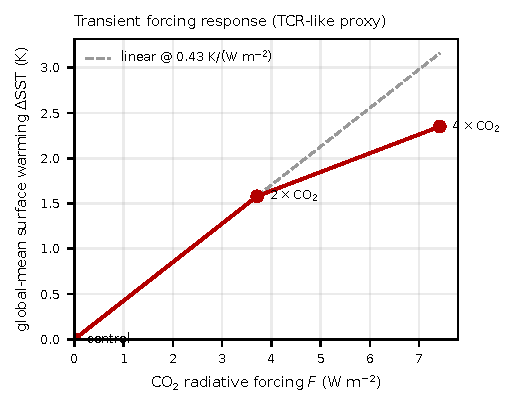
\includegraphics[width=0.7\linewidth]{forcing_response}
\caption{Transient global-mean surface warming $\Delta\SST$ versus CO\textsubscript{2}
radiative forcing for the abrupt-$2\times$ and abrupt-$4\times$CO\textsubscript{2}
experiments. The dashed line is the linear response calibrated on the $2\times$ point; the
$4\times$ point falls below it, showing the sub-logarithmic (saturating) forcing response of
the proxy. Regenerate with \code{experiments/plot\_forcing\_response.py}.}
\label{fig:f14_response}
\end{figure}

% ======================================================================
\section*{Exercises}
% ======================================================================

\begin{exercise}[The forcing trap, quantified]
Using Equation~\eqref{eq:f14_balance}, compute the steady SST anomaly that the
\emph{control} restoring ($\Hrest=79\,\mathrm{W\,m^{-2}K^{-1}}$) would permit
under $2\times$CO\textsubscript{2}, and compare it with the
$0.65\,\mathrm{W\,m^{-2}K^{-1}}$ free mode. By what factor does freeing the ocean
increase the permitted steady response? Explain in one sentence why this factor
is \emph{not} the same as the ratio of the actual simulated warmings, and which
two physical processes (in the transient run) break the simple proportionality.
\end{exercise}

\begin{exercise}[A forcing sweep]
Run \code{experiments/run\_dino\_co2.py} for $C\in\{420,560,1120\}\,\mathrm{ppm}$
against the $280\,\mathrm{ppm}$ baseline. For each, record $\Forc$ from
Equation~\eqref{eq:f14_myhre} and the simulated $\Delta\SST$. Plot $\Delta\SST$
against $\Forc$ (not against $C$). Is the relationship linear? Fit a slope and
compare it with Equation~\eqref{eq:f14_result}. What does the logarithmic form of
Equation~\eqref{eq:f14_myhre} imply for the spacing of your three points on the
\emph{concentration} axis versus the \emph{forcing} axis?
\end{exercise}

\begin{exercise}[Drift cancellation matters]
The experiment defines warming as a difference of two branches
(Equation~\eqref{eq:f14_dSST}). Re-derive $\Delta\SST$ from the single forced
branch alone (do \emph{not} subtract the baseline) and compare. Estimate the
residual drift of the free model from the baseline curve and argue, with numbers,
whether ignoring it would have changed the headline
$0.43\,\mathrm{K\,(W\,m^{-2})^{-1}}$ by more than its honest uncertainty.
\end{exercise}

\begin{exercise}[From two runs to one gradient]
The Myhre forcing is differentiable in $C$. Sketch how you would obtain
$\mathrm{d}\Delta\SST/\mathrm{d}C$ at $C=560\,\mathrm{ppm}$ using \code{jax.grad}
through \code{ocean\_fluxes\_jax} rather than by finite-differencing two 50-year
integrations. Which term in the surface budget carries the gradient, and which
two terms (the frozen $\Qflux$ and the area-mean removal) contribute zero or a
constant to it? Cross-reference your answer with
Chapter~\ref{chap:ch15_differentiable_applications}.
\end{exercise}

\chapter{Differentiable Applications: Calibration, Sensitivity, Data Assimilation}
\label{chap:ch15_differentiable_applications}

% --- local symbols (minimal; not in the shared preamble) ---
\providecommand{\Jcost}{\mathcal{J}}          % cost / objective functional
\providecommand{\dST}{\Delta S}               % subpolar-minus-subtropical salinity contrast
\providecommand{\Fcrit}{F_{\mathrm{crit}}}    % saddle-node freshwater flux
\providecommand{\param}{\boldsymbol{\theta}}  % parameter vector

The defining feature of \model{} is that every prognostic step --- ocean tracer
advection, the \dino{} spectral atmosphere, the bulk flux coupler, the
overturning closure --- is written as a composition of \jax{} primitives, so the
\emph{entire} coupled trajectory is a differentiable function of its inputs
\citep{jax2018}. Chapters \ref{chap:ch03_differentiable}--\ref{chap:ch14_forcing_response}
built this machine; this chapter shows what the derivatives are \emph{for}. We
treat four concrete uses --- gradient-based parameter calibration, sensitivity
maps, four-dimensional variational data assimilation (4D-Var), and the calibration
of a tipping point --- and we are deliberately honest about the one place where
naive backpropagation \emph{fails}: a bifurcation is non-smooth, and the gradient
through a long integration that crosses it diverges. The remedy, fold
continuation by implicit differentiation, closes the chapter and forward-references
the AMOC tipping study of Chapter \ref{chap:ch17_amoc_tipping}.

\section{The differentiable model as a function}

Write the coupled step (Chapter \ref{chap:ch13_coupler_fluxes}) as a map
$\mathbf{x}_{n+1} = \mathcal{M}(\mathbf{x}_n;\param)$, where $\mathbf{x}$ is the
state pytree (ocean \code{OceanState}, \dino{} modal \code{pe.State}, land, ice)
and $\param$ collects tunable parameters. The forward model over $N$ coupling
intervals is the composition $\mathcal{M}^{N}$. A scalar objective
$\Jcost(\mathbf{x}_0,\param)$ --- a misfit to observations, a climatology error,
or a target diagnostic --- is therefore an ordinary differentiable function, and
\jax{} returns its exact gradient by reverse-mode AD (the adjoint):
\begin{equation}
  \nabla_{\param}\Jcost
  \;=\; \code{jax.grad}(\Jcost)(\param),
  \qquad
  \nabla_{\mathbf{x}_0}\Jcost
  \;=\; \code{jax.grad}(\Jcost,\,\mathrm{argnums}{=}0)(\mathbf{x}_0).
  \label{eq:adgrad}
\end{equation}
This is not a finite-difference estimate: it is the analytic derivative of the
discrete program, accurate to floating point. The coupled step is built so this
works in practice. Each interval is
\codref{chronos\_esm/coupler/dino\_step.py}{\code{DinoCoupledModel.\_advance}: SST
$\to$ regrid $\to$ \dino{} interval $\to$ flux coupler $\to$ ocean \code{scan}},
and the differentiable variant \code{step()} wraps both the atmosphere interval
and the inner ocean sub-stepping in \code{jax.checkpoint} (rematerialisation) so
the reverse pass stores only interval-boundary states and recomputes the rest:
\begin{equation}
  \underbrace{\text{store every step}}_{\text{memory }\mathcal{O}(N_{\mathrm{sub}})}
  \;\longrightarrow\;
  \underbrace{\text{store boundaries, recompute}}_{\text{memory }\mathcal{O}(1),\ \text{cost }\times 2}.
  \label{eq:remat}
\end{equation}
The two code paths are intentionally split: \code{step\_fast} is one fused
\code{jit} program with \emph{no} remat (used for forward control/forced runs,
$\sim 10\times$ faster), while \code{step} carries the remat for gradients and DA.

\begin{remark}
Reverse mode costs $\mathcal{O}(1)$ adjoints regardless of the number of
parameters, so it is the right tool for high-dimensional control vectors (an
initial-condition field, a 3-D flux correction). For a handful of scalar
parameters, forward-mode (\code{jax.jvp}) or even central differences are
competitive and easier to validate against.
\end{remark}

\section{Gradient-based parameter calibration}

Calibration tunes $\param$ so the model reproduces data. The classical
approach perturbs each parameter and reruns; with $P$ parameters this is
$P{+}1$ runs per gradient step. Differentiability collapses that to \emph{one}
run plus one adjoint, \emph{independent of $P$}. Given targets
$\mathbf{y}_k$ (e.g.\ WOA18 SST/SSS \citep{locarnini2018woa,zweng2018woa}, ERA5 winds \citep{hersbach2020era5}) sampled by an observation
operator $\mathcal{H}$, minimise
\begin{equation}
  \Jcost(\param)
  = \sum_k \big\lVert \mathcal{H}\big(\mathcal{M}^{k}(\mathbf{x}_0;\param)\big)
      - \mathbf{y}_k \big\rVert^{2}_{\mathbf{R}^{-1}}
  \;+\; \tfrac12\,\lVert \param - \param_b\rVert^{2}_{\mathbf{B}^{-1}},
  \label{eq:calib}
\end{equation}
with $\mathbf{R}$ the observation-error covariance and the second term a
background (prior) regulariser around $\param_b$ with covariance $\mathbf{B}$.
Any \jax{}-compatible optimiser (L-BFGS, Adam) then iterates
$\param \leftarrow \param - \alpha\,\nabla_{\param}\Jcost$ using
\eqref{eq:adgrad}. Natural targets in \model{} are the eddy-diffusivity
$\kappa_{\mathrm{GM}}$ \citep{gentmcwilliams1990}, the bulk drag coefficient,
hyperdiffusion coefficients, and the overturning closure constants
($\code{thc\_k\_vel}$, $\code{thc\_haline\_gain}$) threaded through
\code{\_advance}.

\begin{remark}[Gradient hygiene over long windows]
The adjoint of a chaotic trajectory has a Lyapunov-amplified component: the
gradient is correct for the \emph{discrete} cost, but its variance grows with
window length and it stops being a useful descent direction for a
\emph{climatological} target. Keep calibration windows short (days--weeks for the
atmosphere), or target time-mean / low-frequency statistics, or use the
steady-state route of \S\ref{sec:fold}. This is the same caveat that motivates
fold continuation below.
\end{remark}

\section{Sensitivity maps}

A sensitivity map is the spatial gradient field of a scalar diagnostic with
respect to a field-valued input --- exactly the by-product of one adjoint.
Let $J$ be, say, the AMOC strength at $26.5^\circ$N (Chapter
\ref{chap:ch08_ocean_overturning}) and let the input be the surface freshwater
flux $F(\lat,\lon)$. Then
\begin{equation}
  \frac{\delta J}{\delta F(\lat,\lon)}
  = \big[\code{jax.grad}(J)(F)\big](\lat,\lon)
  \label{eq:sensmap}
\end{equation}
is a 2-D field telling you \emph{where} a unit of freshwater most weakens (or
strengthens) the overturning. One reverse pass yields the sensitivity to every
grid point at once --- the property that makes adjoint sensitivity the workhorse
of ocean state estimation. Because the barotropic streamfunction solve sits
inside the ocean step, these maps propagate through an \emph{implicit} linear
solve; the next section explains why that is differentiable for free.

\subsection*{Differentiating through the elliptic solve}

The ocean streamfunction is obtained by solving a variable-coefficient elliptic
problem (Chapter \ref{chap:ch07_ocean_prognostic_core}),
\begin{equation}
  \diver\!\big(\kappa\,\grad\psib\big) = \vort,
  \qquad \kappa = 1/\dep,
  \label{eq:elliptic}
\end{equation}
on the sphere, discretised in symmetric face-conductance form so the operator is
SPD and solved by a custom conjugate-gradient (CG) iteration,
\codref{chronos\_esm/ocean/solver.py}{\code{solve\_elliptic\_varcoef\_sphere} /
\code{solve\_cg}}. Two design choices make \eqref{eq:elliptic} differentiable.
First, the CG loop uses \code{jax.lax.scan} for a \emph{fixed} \code{max\_iter}
with a \code{jnp.where} that turns converged steps into no-ops --- a
\code{while\_loop} would not be reverse-differentiable:
\begin{equation}
  \mathbf{x}^{(i+1)} =
  \begin{cases}
    \mathbf{x}^{(i)}, & r^{(i)} \le \mathrm{tol}\cdot\lVert b\rVert \quad(\text{no-op}),\\[2pt]
    \mathbf{x}^{(i)} + \alpha_i\,\mathbf{p}^{(i)}, & \text{otherwise},
  \end{cases}
  \qquad
  \alpha_i = \frac{\mathbf{r}^{(i)\!\top}\mathbf{z}^{(i)}}{\mathbf{p}^{(i)\!\top}A\mathbf{p}^{(i)}}.
  \label{eq:cgstep}
\end{equation}
Second, the operator pins $\psib=0$ on land via an identity row
($A_{ii}=1$ there) rather than masking faces, which would make $A$ singular and
the CG diverge --- a Dirichlet ($\psib=0$) coastline is the correct
streamfunction boundary condition. Because the solution satisfies $A\psib=b$
with $A,b$ depending on $\param$, the adjoint of the solve is itself a solve of
$A^{\top}\boldsymbol{\lambda}=\partial J/\partial\psib$; AD through the unrolled
\code{scan} computes this automatically (a small floor \code{1e-12} guards the
Jacobi preconditioner and the $\alpha_i$ denominator against division by zero).

\section{Variational data assimilation (4D-Var) on the atmosphere}

4D-Var seeks the initial state $\mathbf{x}_0$ that best fits a window of
observations subject to the model dynamics as a strong constraint. With the
\dino{} atmosphere as the active dynamical core
(\codref{chronos\_esm/coupler/dino\_step.py}{\code{DinoCoupledModel.step}, the
remat'd differentiable interval}), the standard incremental cost is
\begin{equation}
  \Jcost(\mathbf{x}_0) =
  \tfrac12 \lVert \mathbf{x}_0 - \mathbf{x}_b \rVert^{2}_{\mathbf{B}^{-1}}
  + \tfrac12 \sum_{k=0}^{K}
    \big\lVert \mathcal{H}_k\!\big(\mathcal{M}^{k}(\mathbf{x}_0)\big) - \mathbf{y}_k
    \big\rVert^{2}_{\mathbf{R}_k^{-1}},
  \label{eq:4dvar}
\end{equation}
with $\mathbf{x}_b$ the background, $\mathbf{B},\mathbf{R}_k$ the background and
observation error covariances. The control variable is the modal \dino{} state
(vorticity / divergence / temperature variation / log-surface-pressure), which is
a registered \jax{} pytree and therefore a legal argument to \code{jax.grad}. The
gradient
\begin{equation}
  \nabla_{\mathbf{x}_0}\Jcost
  = \mathbf{B}^{-1}(\mathbf{x}_0-\mathbf{x}_b)
  + \sum_k \mathbf{M}_k^{\top}\,\mathbf{H}_k^{\top}\,\mathbf{R}_k^{-1}
    \big(\mathcal{H}_k(\mathbf{x}_k)-\mathbf{y}_k\big)
  \label{eq:4dvargrad}
\end{equation}
involves the tangent-linear $\mathbf{M}_k=\partial\mathcal{M}^{k}/\partial\mathbf{x}_0$
and its adjoint $\mathbf{M}_k^{\top}$ --- in a hand-coded DA system these are
thousands of lines of separately maintained code that must be re-validated every
time the forward model changes. Here they are \emph{generated} by reverse-mode AD
of the same forward step, so they can never drift out of sync with the model.
\begin{example}[A minimal atmospheric 4D-Var]
Build the model once, then minimise \eqref{eq:4dvar} over a short window:
\begin{lstlisting}[style=chronos]
model = DinoCoupledModel()                  # dino atmosphere active
def J(atmos0):
    st = state0._replace(atmos=atmos0)
    miss = 0.0
    for k in range(K):
        st = model.step(st, interval=0.25)  # 6-h slot, remat'd
        miss += loss(model.diagnostics_lin(st), y[k])
    return Jb(atmos0) + miss
g = jax.grad(J)(state0.atmos)               # adjoint of the whole window
\end{lstlisting}
The atmosphere is the cleanest 4D-Var target in \model{}: short windows, a
genuine multi-level dynamical core, and well-behaved tangent linearity over a few
days. Ocean and fully coupled DA are gated by the slower, stiffer ocean adjoint
and are out of scope here.
\end{example}

\section{Bifurcations are non-smooth: calibrate the fold, not the run}
\label{sec:fold}

The applications above all assume the objective is a smooth function of the
trajectory. A \emph{tipping point} breaks that assumption. The AMOC `on'/`off'
collapse is a saddle-node (fold) bifurcation \citep{stommel1961,rahmstorf2005}:
as a control parameter --- here the North-Atlantic freshwater (hosing) flux $F$
--- crosses a critical value $\Fcrit$, the stable on-state \emph{ceases to exist}
and the system jumps to the off-state. Two facts make
``$\code{jax.grad}$ through a 200-year hosing sweep'' the wrong tool:
\begin{enumerate}
  \item the trajectory sensitivity $\partial\mathbf{x}/\partial F$
        \emph{diverges} as $F\to\Fcrit$ (the linearisation has a zero eigenvalue
        at the fold), so the backpropagated gradient blows up exactly where you
        need it;
  \item even away from the fold you would differentiate through hundreds of model
        years and a discrete collapse event --- expensive and dominated by the
        chaotic tail of \S3.
\end{enumerate}
The rigorous differentiable handle on a fold is \emph{continuation}: implicitly
differentiate the joint conditions that \emph{define} the fold rather than
backpropagating a trajectory.

\subsection*{The reduced box and its fold}

\model{}'s overturning closure
(\codref{chronos\_esm/ocean/overturning.py}{\code{thc\_overturning\_velocity}})
sets the AMOC amplitude from an Atlantic upper-ocean density contrast through a
$\softplus$ rectifier,
\begin{equation}
  A \;=\; C_{\mathrm{eff}}\,k_{\mathrm{rel}}\,
          \softplus\!\Big(\frac{\Delta\dens + (\gamma-1)\,\beta_S\,\dST}{\delta\rho}\Big),
  \qquad
  \softplus(z)=\log(1+e^z),
  \label{eq:amocclosure}
\end{equation}
where $\Delta\dens$ is the thermal density contrast, $\dST$ the subpolar-minus-
subtropical salinity contrast, $\gamma=\code{haline\_gain}$ amplifies the haline
feedback, $\beta_S=0.78\ \mathrm{kg\,m^{-3}\,psu^{-1}}$, $\delta\rho=0.1$, and
$k_{\mathrm{rel}}=k_{\mathrm{vel}}/10^{-4}$. The calibration script
\codref{experiments/calibrate\_amoc\_fold.py}{\code{amoc} / \code{fcrit} /
\code{newton\_invert}} recognises that, with a salt-advection feedback, this
closure \emph{is} a Stommel two-box model. Reducing to the salinity contrast
$s\equiv\dST$ with thermal contrast held fixed,
\begin{align}
  \dt{s} &= -\kappa F \;+\; \mu\,A(s)\,(-s), \label{eq:boxode}\\
  A(s)   &= C_{\mathrm{eff}}\,k_{\mathrm{rel}}\,
            \softplus\!\Big(\frac{\rho_T + \gamma\,\beta_S\,s}{\delta\rho}\Big),
            \label{eq:boxamoc}
\end{align}
where hosing $F$ freshens the box ($-\kappa F$) and the overturning imports salt
at a rate $\propto A(s)(-s)$ (advective feedback: a stronger AMOC carries more
salt poleward, deepening the contrast). The steady on-state balances these,
$\kappa F = \mu A(s)(-s) =: R(s)$, and since $R(s)\to0$ as $s\to0^-$ and as
$s\to-\infty$, $R$ has an interior maximum. That maximum is the fold:
\begin{equation}
  \boxed{\;\Fcrit(\param)\;=\;\max_{s}\;\frac{R(s)}{\kappa}
        \;=\;\frac{\mu}{\kappa}\,\max_{s}\,A(s)\,(-s)\;}
  \label{eq:fcrit}
\end{equation}
For $F>\Fcrit$ no steady on-state exists: the saddle and node have annihilated.

\subsection*{Why AD of the fold is exact: the envelope theorem}

The key step is that $\Fcrit$ is itself a \emph{maximum} over the internal
coordinate $s$. By the envelope theorem, the parameter-derivative of a maximised
function equals the partial derivative at the optimum, with the
$\partial(\cdot)/\partial s\cdot\dd s^\star/\dd\param$ term vanishing because
$\partial R/\partial s=0$ there (that vanishing condition is exactly the fold's
zero-eigenvalue condition):
\begin{equation}
  \frac{\dd \Fcrit}{\dd \param}
  = \left.\frac{1}{\kappa}\,\pd{R}{\param}\right|_{s=s^\star(\param)} .
  \label{eq:envelope}
\end{equation}
So differentiating the \emph{discretised} $\max$ over a fixed grid $\_S\_GRID$
($s\in[-3,-0.02]$, $4000$ points; \code{jnp.max} after a \code{vmap}) gives the
correct fold gradient to machine precision --- no integration, no divergence, one
\code{jax.grad}. The script then \emph{inverts}: given a target $\Fcrit$ (default
$0.6\Sv$), Newton's method on \eqref{eq:fcrit} with an AD-supplied derivative
solves for the parameter (here \code{haline\_gain}) that places the fold there,
\begin{equation}
  \gamma^{(i+1)} = \gamma^{(i)}
   - \frac{\Fcrit(\gamma^{(i)}) - \Fcrit^{\mathrm{target}}}
          {\dd\Fcrit/\dd\gamma\big|_{\gamma^{(i)}}},
  \label{eq:newton}
\end{equation}
\codref{experiments/calibrate\_amoc\_fold.py}{\code{newton\_invert}: 15 AD-Newton
iterations}. The two lumped box constants $C_{\mathrm{eff}}$ and $\mu/\kappa$ are
first fitted to GCM anchors --- the on-state AMOC at $F{=}0$ fixes
$C_{\mathrm{eff}}$, a near-marginal hosing run fixes $\mu/\kappa$ --- read from
saved hysteresis sweeps (\code{\_load\_anchors}). One confirmatory full GCM hosing
run then validates the predicted $\Fcrit$, replacing an entire multi-job parameter
grid with a single run.

\begin{remark}[Honest scope]
The reduction \eqref{eq:boxode}--\eqref{eq:boxamoc} is a \emph{caricature}: a
single salinity contrast, fixed thermal contrast, lumped constants. Its value is
that it shares the \emph{functional form} \eqref{eq:amocclosure} of the GCM
closure, so the fold it predicts is a calibrated \emph{guess} for where the full
model tips --- not a substitute for the full hysteresis experiment. The
envelope-theorem gradient is exact for the box; whether the box's $\Fcrit$
matches the GCM's is an empirical question answered by the confirmatory run.
Chapter \ref{chap:ch17_amoc_tipping} carries this through to the full coupled
hysteresis and its interpretation.
\end{remark}

\begin{remark}[$\softplus$ as a differentiable rectifier]
A hard threshold $\max(0,\cdot)$ on the density contrast would give a
non-differentiable (and, with a hard on/off, a genuinely discontinuous)
overturning. The $\softplus$ in \eqref{eq:amocclosure} is a smooth surrogate:
positive and $C^\infty$, with $\softplus(z)\approx z$ for $z\gg0$ and
$\softplus(z)\approx e^{z}\to 0$ for $z\ll0$. It keeps the closure
differentiable everywhere \emph{within} a branch; the non-smoothness that matters
is the fold \eqref{eq:fcrit} between branches, which is why it needs continuation,
not a smoother rectifier.
\end{remark}

\section*{Summary}

Differentiability turns calibration from a parameter grid into a gradient
descent, turns sensitivity studies into a single adjoint, and supplies the
tangent-linear and adjoint operators of 4D-Var for free
\citep{jax2018,kochkov2024neuralgcm}. The one structural caveat is the
bifurcation: backpropagation through a trajectory that crosses a fold diverges,
and the correct differentiable object is the fold condition itself, handled by
implicit differentiation and the envelope theorem on a reduced box. The same
adjoint that makes the smooth applications cheap is what forces this distinction
to be made explicit.

\begin{exercise}[Sensitivity to the drag coefficient]
Using \code{DinoCoupledModel.step}, define $J$ as the global-mean kinetic energy
of the surface ocean after a 30-day integration and compute
$\partial J/\partial C_d$ with \code{jax.grad}. Verify the AD gradient against a
central finite difference $\big(J(C_d{+}\epsilon)-J(C_d{-}\epsilon)\big)/2\epsilon$
for $\epsilon=10^{-3}$. Explain any disagreement in terms of the remat path and
the CG tolerance in \code{solve\_cg}.
\end{exercise}

\begin{exercise}[Freshwater sensitivity map]
Take $J$ = AMOC at $26.5^\circ$N (Chapter \ref{chap:ch08_ocean_overturning}) and
compute the field $\delta J/\delta F(\lat,\lon)$ via \eqref{eq:sensmap} over a
5-year window. Where is the AMOC most sensitive to freshwater forcing? Compare
the location of the maximum-magnitude sensitivity with the subpolar
North-Atlantic deep-water-formation region implied by the convection layer in
\code{thc\_overturning\_velocity}.
\end{exercise}

\begin{exercise}[Reproduce the fold calibration]
Run \code{python experiments/calibrate\_amoc\_fold.py --target 0.6}. (i) From the
printed $\Fcrit$ table over $(\code{haline\_gain},k_{\mathrm{vel}})$, confirm that
$\Fcrit$ increases with the haline gain and decreases with $k_{\mathrm{vel}}$, and
explain both signs from \eqref{eq:fcrit}. (ii) Re-derive the AD gradient
$\dd\Fcrit/\dd\gamma$ at the solution using \eqref{eq:envelope} and check it
against the script's value. (iii) Why does refining \code{\_S\_GRID} from 4000 to
40\,000 points barely change $\Fcrit$, whereas \emph{shrinking} its range to
exclude $s^\star$ corrupts it?
\end{exercise}

\begin{exercise}[Why not backprop the sweep?]
Argue quantitatively that $\partial(\text{AMOC}_{26.5})/\partial F$ from a
hosing-sweep adjoint must diverge as $F\to\Fcrit^-$. Relate the divergence to the
zero eigenvalue of the steady-state Jacobian at the fold, and contrast with the
\emph{finite} envelope-theorem derivative \eqref{eq:envelope}. What does this
imply for the variance of a 4D-Var gradient \eqref{eq:4dvargrad} computed over a
window that straddles a tipping event?
\end{exercise}


\part{Canonical Climate Test Cases}
\chapter{Mean Climatology versus Observations}
\label{chap:ch16_climatology}

\emph{[This chapter is under construction.]}

\chapter{The AMOC: Overturning, Hosing, and Tipping}
\label{chap:ch17_amoc_tipping}

The Atlantic Meridional Overturning Circulation (AMOC) carries warm, salty water poleward in
the upper Atlantic and returns cold, dense water at depth. It is a textbook example of a climate
\emph{tipping element}: theory and a hierarchy of models suggest the overturning can collapse
abruptly and \emph{irreversibly} once a freshwater perturbation exceeds a critical threshold,
because of the salt-advection feedback first identified by \citet{stommel1961}. This chapter
uses \model{} as a laboratory to reproduce that bifurcation, and --- exploiting
differentiability --- to \emph{calibrate} where it occurs. The governing equations of the
overturning closure are given in Chapter~\ref{chap:ch08_ocean_overturning}; here we focus on the
experiments and results.

\section{The salt-advection feedback}

Write the overturning strength $q$ as an increasing function of the meridional density contrast
between the subpolar and subtropical Atlantic. A stronger $q$ imports more salt to the subpolar
basin, raising its density, which strengthens $q$ further: a positive feedback. A subpolar
freshwater input (``hosing'') opposes it. When the feedback loop gain exceeds unity the system
becomes \emph{bistable} --- an ``on'' (vigorous) and an ``off'' (collapsed) state coexist over a
finite range of forcing --- and the transition between them is a saddle-node bifurcation with
hysteresis. In \model{} the loop gain is set by the tunable parameter \code{haline\_gain}
(Chapter~\ref{chap:ch08_ocean_overturning}).

\section{The hosing experiment}

We add a freshwater flux $F$ (in Sverdrups, $1\Sv=10^6~\mathrm{m^3\,s^{-1}}$) over the
$45$--$65^\circ$N Atlantic surface and record the AMOC strength at $26.5^\circ$N. Two protocols
are used:

\begin{description}[leftmargin=0pt,style=nextline]
  \item[Quasi-static sweep] Ramp $F$ slowly up ($0\!\to\!F_{\max}$) then down
    ($F_{\max}\!\to\!0$), holding each level to near-equilibrium. An open loop (the down-leg
    below the up-leg) signals hysteresis. \emph{Caveat:} near the fold the collapse timescale is
    multi-decadal, so finite holds give a \emph{rate-dependent} loop that can be mistaken for, or
    hide, true bistability.
    \codref{experiments/run\_amoc\_hosing.py}{quasi-static hosing sweep}
  \item[Fixed-$F$ bistability test] The rigorous protocol: at a single fixed $F$, integrate one
    run started from an \emph{on}-state and one from an \emph{off}-state for $\sim100$~years. If
    the two converge, the system is monostable at that $F$; if they remain separated, it is
    genuinely bistable. This is immune to rate-dependence.
    \codref{experiments/run\_amoc\_bistability.py}{fixed-$F$ on/off initial-condition test}
\end{description}

\section{A verified bistable window}

With the calibrated configuration \code{haline\_gain}$=6$, \code{thc\_k\_vel}$=6\times10^{-5}$,
and a convection-layer contrast depth of $300$~m, the fixed-$F$ test gives the result in
Table~\ref{tab:amoc_bist} and Figure~\ref{fig:amoc_bist}. At $F=0.46,\,0.57,\,0.69\Sv$ the
on-state and off-state branches remain $8$--$9\Sv$ apart after $100$~years --- a separation that
is statistically significant (autocorrelation-corrected $z=2.6$--$4.4$) and persistent (the
off-branch does not recover). Below $F\approx0.3\Sv$ an off-state initial condition recovers to
the upper branch; above $F\approx0.8\Sv$ an on-state initial condition collapses. The
\emph{hysteresis window} is therefore approximately
\[
  F_{\mathrm{lower}} \approx 0.38\Sv \;<\; F \;<\; F_{\mathrm{upper}} \approx 0.75\Sv,
\]
centered near $0.6\Sv$ --- consistent with the freshwater-transport scale of a $\sim15$--$20\Sv$
AMOC and with the collapse thresholds reported across the model hierarchy
\citep{rahmstorf2005}.

\begin{table}[h]
\centering
\caption{Equilibrated AMOC (last-40-yr mean) at $26.5^\circ$N from on-state vs.\ off-state
initial conditions, held at fixed hosing $F$ for $100$~years.}
\label{tab:amoc_bist}
\begin{tabular}{cccc}
\toprule
$F$ (Sv) & ON-branch (Sv) & OFF-branch (Sv) & separation $z$ \\
\midrule
$\le 0.30$ & \multicolumn{2}{c}{off-IC recovers to ON} & --- \\
$0.46$ & $\approx 20$ & $\approx 12$ & $2.6$ \\
$0.57$ & $\approx 18$ & $\approx 10$ & $3.1$ \\
$0.69$ & $\approx 15$ & $\approx 6$  & $4.4$ \\
$\ge 0.80$ & \multicolumn{2}{c}{on-IC collapses to OFF} & --- \\
\bottomrule
\end{tabular}
\end{table}

\begin{figure}[h]
\centering
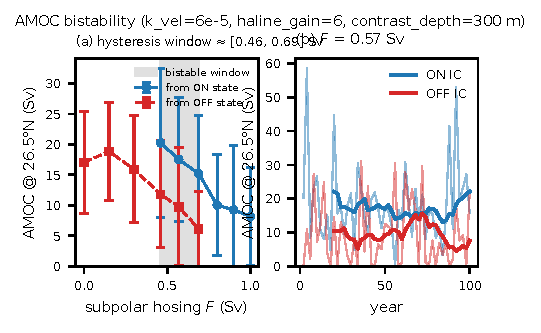
\includegraphics[width=\linewidth]{amoc_bistability}
\caption{The AMOC hysteresis window. (a) On-state (blue) and off-state (red) equilibrated AMOC
versus hosing $F$; the branches stay separated across the window. (b) At $F=0.57\Sv$ the two
initial conditions settle on different branches and do not reconverge over $100$~years ---
the signature of genuine bistability.}
\label{fig:amoc_bist}
\end{figure}

\paragraph{An honest caveat.} The branches are \emph{noisy}: the AMOC oscillates by
$\sim\!\pm10\Sv$ (a relaxation oscillation intrinsic to the strong feedback in this interim
box-style closure). The bifurcation is genuine --- established by the statistically-significant,
non-recovering initial-condition dependence --- but it is not a clean, low-variance loop. A clean
dynamical bifurcation requires the prognostic-momentum ocean core of
Chapter~\ref{chap:ch07_ocean_prognostic_core}; the closure used here \emph{works around}, rather
than solves, the fact that the diagnostic-velocity ocean has $\partial(\mathrm{AMOC})/\partial\rho
\approx 0$.

\section{Calibrating the tipping point by differentiation}

A tipping threshold is a bifurcation, and therein lies a subtlety for differentiable modeling:
one \emph{cannot} obtain $\partial F_{\mathrm{crit}}/\partial\boldsymbol{\theta}$ by
backpropagating through the hosing sweep, because the trajectory's sensitivity \emph{diverges} at
the fold (that divergence \emph{is} the bifurcation). The correct tool is \emph{fold
continuation}: reduce the closure to its governing Stommel box, where the steady-state condition
$F = R(s;\boldsymbol{\theta})$ has a fold at $\partial R/\partial s=0$, so that
$F_{\mathrm{crit}}(\boldsymbol{\theta}) = \max_s R(s;\boldsymbol{\theta})$. By the envelope
theorem the gradient through this maximum is exact, and a few Newton steps invert
$F_{\mathrm{crit}}(\boldsymbol{\theta})=F^\star$ for the parameters in milliseconds --- the
differentiable replacement for a brute-force parameter grid.
\codref{experiments/calibrate\_amoc\_fold.py}{AD fold-continuation calibration}

\noindent
The gradient ranking this yields,
$\partial F_{\mathrm{crit}}/\partial(\code{k\_vel}) \gg
 \partial F_{\mathrm{crit}}/\partial(\code{haline\_gain})$,
shows that the AMOC on-state \emph{strength} is the dominant control on the tipping threshold ---
a non-obvious result that the grid search would have taken hours to reveal.

\section{Reproducing this chapter}

\begin{lstlisting}[language=bash,caption={Hosing sweep, bistability test, and figure.}]
# quasi-static hysteresis sweep (self-contained from WOA; auto-resumes):
python experiments/run_amoc_hosing.py --spinup-years 20 --fmax 0.8 --nsteps 8 \
    --hold-years 15 --haline-gain 6 --k-vel 6e-5 --contrast-depth 300

# rigorous fixed-F bistability test (run once per branch IC, then compare means):
python experiments/run_amoc_bistability.py --ckpt <on_state>  --hosing-sv 0.57 \
    --haline-gain 6 --k-vel 6e-5 --contrast-depth 300 --years 100 --outdir out/on
python experiments/run_amoc_bistability.py --ckpt <off_state> --hosing-sv 0.57 \
    --haline-gain 6 --k-vel 6e-5 --contrast-depth 300 --years 100 --outdir out/off

# differentiable calibration of the threshold, and the figure:
python experiments/calibrate_amoc_fold.py --target 0.6
python experiments/plot_amoc_bistability.py --root out --out docs/figures/amoc_bistability.pdf
\end{lstlisting}

\begin{exercise}
Re-run the fixed-$F$ test at $F=0.57\Sv$ but lower \code{haline\_gain} to $4$. Is the system still
bistable? Relate your answer to the loop-gain condition for bistability.
\end{exercise}

\begin{exercise}
Using \code{calibrate\_amoc\_fold.py}, find the \code{(haline\_gain, k\_vel)} pair that places the
collapse threshold at exactly $F_{\mathrm{crit}}=0.5\Sv$. Verify with one fixed-$F$ run near your
predicted threshold.
\end{exercise}

\begin{exercise}[Differentiability]
Explain in one paragraph why $\partial F_{\mathrm{crit}}/\partial\boldsymbol{\theta}$ cannot be
computed by automatic differentiation \emph{through} a hosing sweep that crosses the fold, and how
fold continuation circumvents the problem.
\end{exercise}

\chapter{Mid-Latitude Jets and Storm Tracks}
\label{chap:ch18_jets_stormtracks}

\emph{[This chapter is under construction.]}

\chapter{The Tropics: ITCZ, Monsoons, and Variability}
\label{chap:ch19_tropics_monsoon}

The tropics are the engine room of the climate system. Solar heating peaks near the equator,
moist convection lofts that heat into the upper troposphere, and the resulting Hadley
circulation exports it poleward. The narrow, deep-convecting rain band where the trade winds of
the two hemispheres meet --- the \emph{Intertropical Convergence Zone} (ITCZ) --- is the single
most prominent feature of the observed precipitation field, and one of the hardest for a coarse
model to capture. This chapter evaluates how \model{} represents the tropical mean state: the
ITCZ and its precipitation, what role the multi-level moist atmosphere plays in producing it,
and --- honestly --- where the representation remains weak, including the near-absence of
interannual (ENSO-like) variability and the limited monsoon at this resolution.

This is a Part~IV evaluation chapter. We first define the phenomenon and the physics that should
produce it, recall how the relevant model components implement that physics
(Chapters~\ref{chap:ch09_atmosphere_multilevel} and \ref{chap:ch10_atmosphere_singlelevel}),
describe the diagnostic and the skill metric, then present the validation figures and a
qualitative assessment with its limitations.

\section{The phenomenon: deep convection and the ITCZ}

In the time mean, the trade-wind boundary layers of the Northern and Southern Hemispheres
converge in the deep tropics, forcing ascent, condensation, and a band of intense rainfall. The
ascending branch of the Hadley cell sits over this band; the descending branches dry the
subtropics, producing the desert latitudes near $\pm25^\circ$. The position and strength of the
ITCZ are set by the cross-equatorial energy transport and by the underlying sea-surface
temperature (SST), since deep convection switches on only above an SST threshold of roughly
$26$--$27^\circ$C \citep{vallis2017}. A faithful tropical climate therefore requires two
ingredients simultaneously: a moist atmosphere that can convect and rain, and an ocean whose
tropical SST is warm enough to trigger that convection.

\section{Why vertical structure matters: single level vs.\ multi-level}

The distinction between \model{}'s two atmospheres is sharpest in the tropics. The
\textbf{single-level (barotropic) atmosphere} of Chapter~\ref{chap:ch10_atmosphere_singlelevel}
has no vertical coordinate: it cannot represent the ascent--condensation--latent-heating column
that \emph{is} deep tropical convection. With no resolved Hadley overturning to concentrate
moisture at the equator, its precipitation is too dry and rains in the wrong place --- in the
subtropics and mid-latitudes rather than on the equator --- and its precipitation pattern
correlation against observations is near zero. This is a structural limitation, not a tuning
failure: a single level simply has nowhere to put the vertical motion that makes an ITCZ.

The \textbf{multi-level spectral atmosphere} built on the \dino{} dycore
(Chapter~\ref{chap:ch09_atmosphere_multilevel}) does have the necessary vertical structure. It
carries prognostic specific humidity as an advected tracer, evaporates moisture from the surface
with a bulk formula \citep{largeyeager2004}, and rains out supersaturation through a large-scale condensation closure
that latent-heats the column. As the resolved Hadley circulation spins up, that closure
concentrates rainfall in the deep tropics and dries the subtropics --- a real ITCZ forming
\emph{from the resolved circulation}, with no explicit convection scheme. \model{} therefore
follows the same lineage as NeuralGCM, whose differentiable spectral core \dino{} is
\citep{kochkov2024neuralgcm}. This is the central evaluation message of the chapter: the
multi-level atmosphere produces an equatorial rain band that the single level cannot.

\section{Diagnostic and metric}

The precipitation diagnostic is the column-integrated condensation rate, $P$ (in mm/day),
output by the multi-level atmosphere's moisture physics and regridded from the Gaussian
transform grid to the model's lat--lon grid. We assess it three ways against the GPCP-class
observational climatology bundled with the validation framework
(\code{chronos\_esm/validation/}):

\begin{description}[leftmargin=0pt,style=nextline]
  \item[Spatial map and bias map] $P$, the observed climatology, and their difference
    $P_{\mathrm{model}}-P_{\mathrm{obs}}$, to localize where the model is too wet or too dry.
  \item[Zonal mean] the latitude profile of $\langle P\rangle_\lambda$, model versus
    observations, which isolates the ITCZ peak, its width, and the subtropical minima.
  \item[Scalar scorecard] area-weighted bias, RMSE, pattern correlation, and standard-deviation
    ratio (a perfect model scores bias $0$, corr $1$, std ratio $1$).
\end{description}

\codref{experiments/make\_readme\_figures.py}{precipitation map, zonal mean, and scorecard}

\section{The current validation dashboard}

Figures~\ref{fig:dino_circ}--\ref{fig:precip_bias} are the present tropical validation
dashboard, generated from a short SST-forced spin-up of the multi-level atmosphere on the WOA18
SST climatology \citep{locarnini2018woa}. The quantitative scorecard is refreshed from the latest control run; a 30-year
time mean of the coupled \dino{}\,$\leftrightarrow$\,ocean control is being generated to replace
the short-spin-up numbers quoted below with an equilibrated climatology.

\begin{figure}[h]
\centering
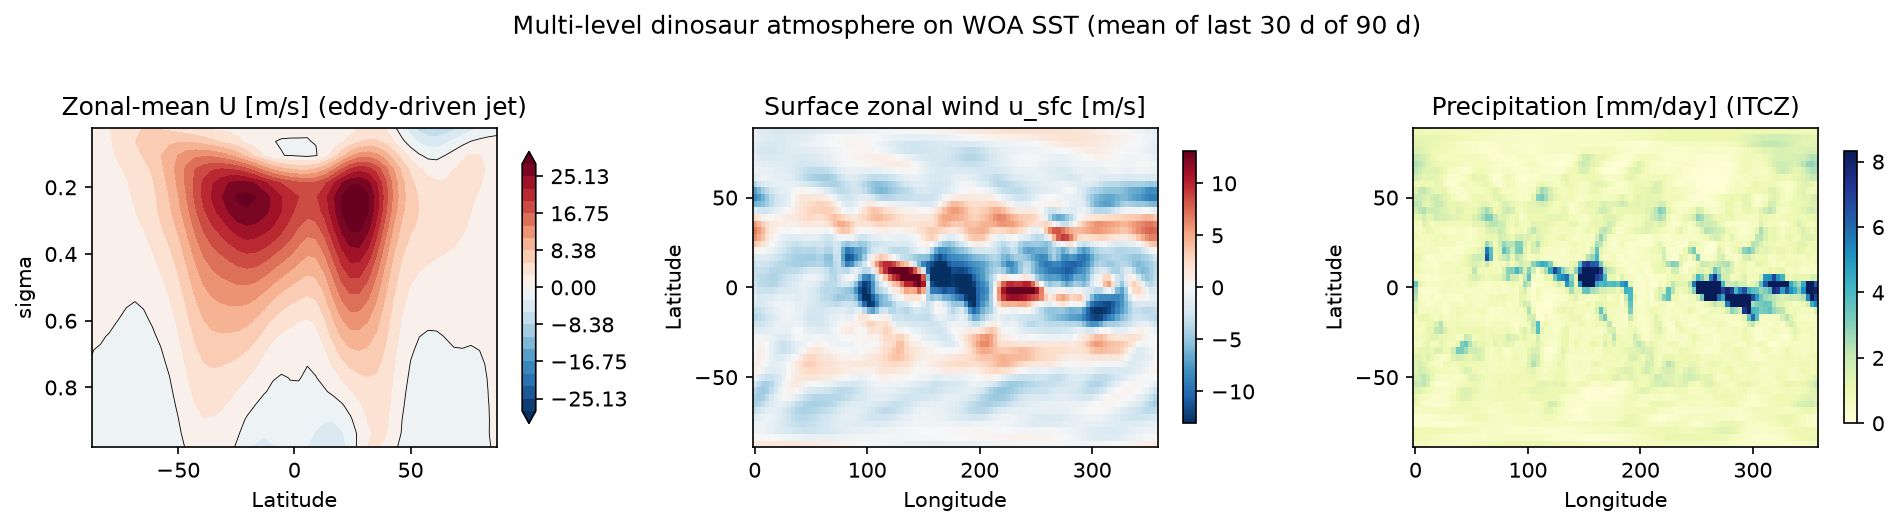
\includegraphics[width=\linewidth]{dino_circulation}
\caption{Multi-level \dino{} atmosphere forced by the WOA SST (time mean of a $120$-day
spin-up). \emph{Left:} the zonal-mean zonal wind, with the twin upper-tropospheric
eddy-driven baroclinic jets ($\sim27$~m/s) that the single level cannot generate. \emph{Centre:}
surface zonal wind, showing trade easterlies straddling the equator. \emph{Right:} precipitation
(mm/day) --- the tropical ITCZ rain band, the feature of interest in this chapter. Regenerate
with \code{python experiments/dino\_circulation\_figure.py}.}
\label{fig:dino_circ}
\end{figure}

The right-hand panel of Figure~\ref{fig:dino_circ} is the headline result: an equatorial band of
enhanced precipitation, organized by the resolved Hadley ascent, with dry subtropical flanks.
The accompanying trade easterlies (centre panel) converging toward that band are the surface
signature of the same circulation. A single-level atmosphere produces neither.

\begin{figure}[h]
\centering

\includegraphics[width=0.72\linewidth]{zonal_precip}
\caption{Zonal-mean precipitation versus latitude: \model{}'s multi-level atmosphere (solid) and
the observed climatology (dashed). The model reproduces a distinct equatorial peak near
$5$--$15^\circ$N --- a genuine ITCZ --- but it is too dry: the peak undershoots the observed
maximum and the subtropical/extratropical totals are low. The single-level atmosphere has no
such equatorial peak.}
\label{fig:precip_zonal}
\end{figure}

\begin{figure}[h]
\centering
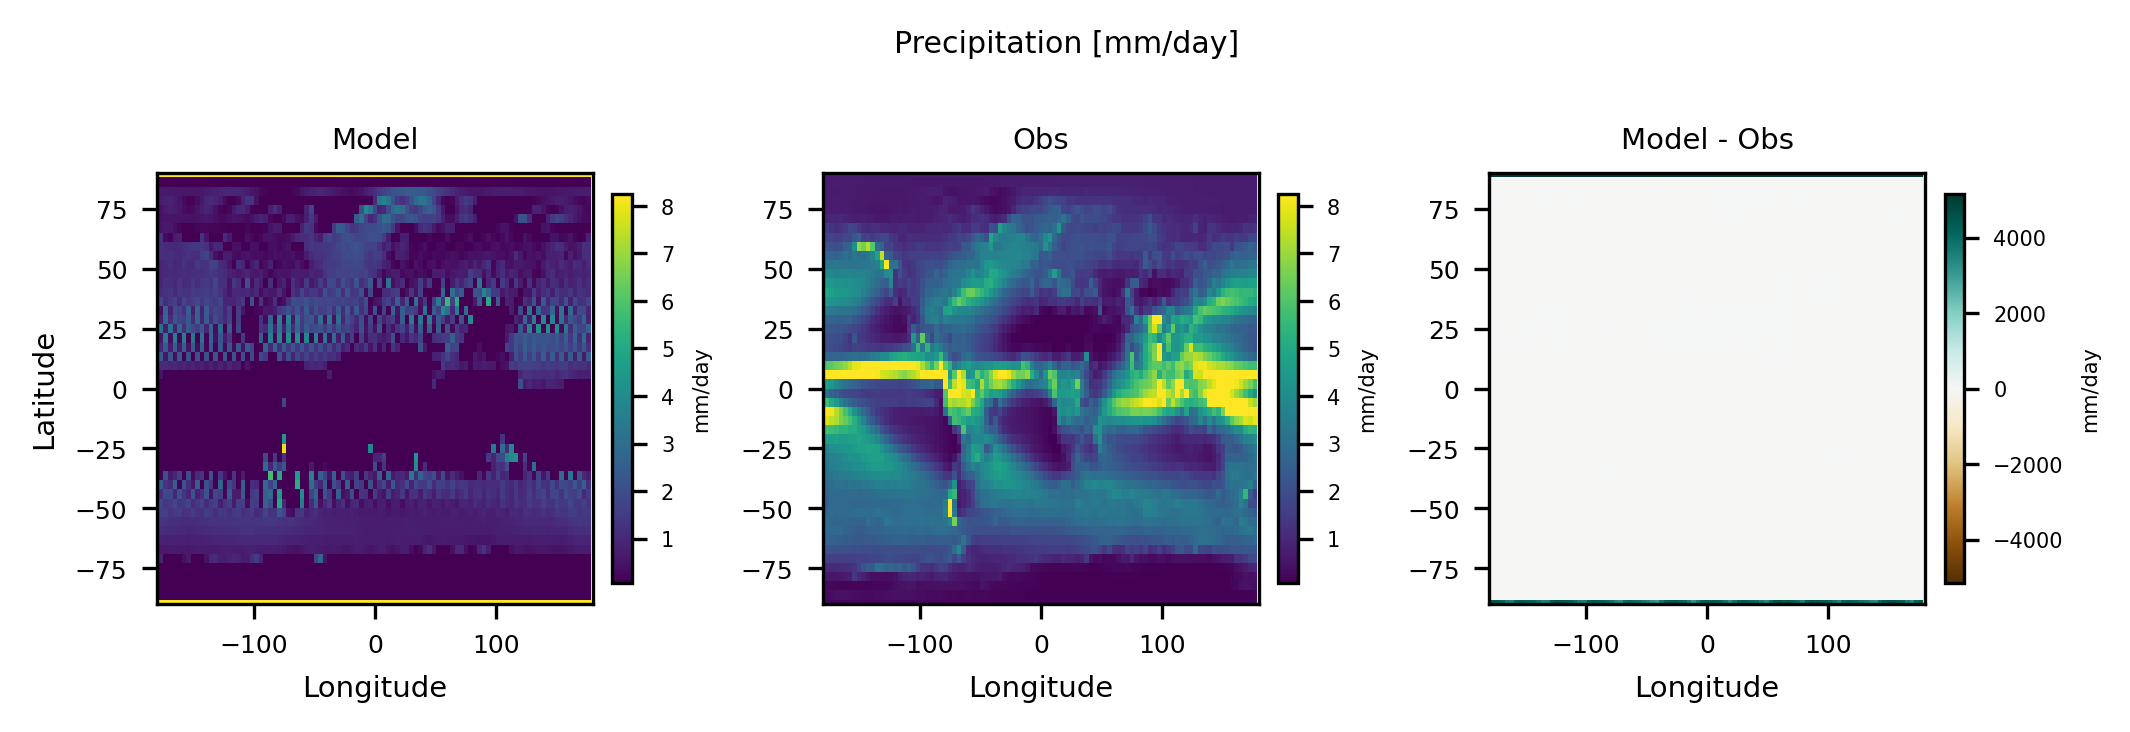
\includegraphics[width=\linewidth]{biasmap_precip}
\caption{Precipitation maps: model (left), observed climatology (centre), and their difference
(right). The model captures the broad equatorial rain band and the Pacific/Atlantic structure,
but is systematically too dry along the deep-tropical maximum (brown band near the equator in the
difference map) and lacks the sharp South Pacific and South Atlantic convergence zones.}
\label{fig:precip_bias}
\end{figure}

\section{Assessment}

\paragraph{What works.} The qualitative win is unambiguous and is documented across the model's
development record. Moving from the single-level to the multi-level moist atmosphere lifts the
precipitation \emph{pattern correlation} markedly: in the SST-forced benchmark it rises from
$0.16$ for the single level to $0.34$ for the multi-level atmosphere, and the precipitation
standard-deviation ratio recovers toward observed (from $0.41$ to $\sim0.8$). Crucially, the
correlation gain comes with a \emph{physically correct} ITCZ --- the model now rains on the
equator instead of in the subtropics. In the fully coupled, flux-corrected control run (where the
tropical SST is restored toward WOA so it is warm enough to convect), the same revival is even
clearer: the precipitation pattern correlation reaches $0.37$, and the documented narrative of
that run names the ``revived ITCZ'' as one of its two headline gains. The chain is exactly the
one the physics predicts in Section~\ref{chap:ch19_tropics_monsoon}: warm tropical SST
$\rightarrow$ deep convection $\rightarrow$ Hadley ascent $\rightarrow$ equatorial rain band.

\paragraph{What does not (yet).} Three honest limitations stand out.

\begin{enumerate}[leftmargin=*]
  \item \textbf{The ITCZ is still too dry and too weak.} Figure~\ref{fig:precip_zonal} shows the
    equatorial peak undershooting the observed maximum, and the bias map
    (Figure~\ref{fig:precip_bias}) shows a coherent dry band straddling the equator. A pattern
    correlation of $\sim0.34$--$0.37$ is a real improvement but is still modest. The large-scale
    condensation closure has no convective organization or explicit deep-convection
    parameterization, and at T31 ($\sim3.75^\circ$) the rain band is only a few grid cells wide,
    so it is unavoidably blurred and under-peaked.
  \item \textbf{Tropical SST limits the convection.} The free-running coupled model carries a
    tropical cold-tongue bias (tropical SST several degrees below WOA), which suppresses the deep
    convection that should drive the ITCZ. The control run quoted above relies on a Haney SST
    restoring \citep{haney1971} toward WOA to remove that bias; the ITCZ is therefore partly \emph{earned} by the
    flux correction rather than freely predicted. A free-running warm tropical SST remains a
    standing target (Chapter~\ref{chap:ch13_coupler_fluxes}).
  \item \textbf{No strong interannual (ENSO-like) variability.} At this configuration \model{}
    has no documented El~Ni\~no--Southern Oscillation. The coupled control is run as a stable,
    flux-corrected, drift-free mean state; the ocean's diagnostic-velocity dynamics and the
    coarse T31 atmosphere do not sustain the coupled Bjerknes feedback that produces ENSO. The
    tropical climate documented here is a \emph{mean-state} evaluation, not a variability one ---
    and the spurious noise that the AMOC closure exhibits (Chapter~\ref{chap:ch17_amoc_tipping})
    should not be mistaken for organized tropical variability.
\end{enumerate}

\paragraph{Monsoons.} Monsoon circulations --- the seasonal land--sea thermal contrast that
reverses the low-level winds and drives summer rainfall over South Asia, West Africa, and the
Americas --- are only weakly represented. Two factors limit them. First, resolution: at
$\sim3.75^\circ$ the land--sea coastlines, orographic barriers (the Tibetan Plateau, the
Ethiopian Highlands), and narrow monsoon rain bands are smoothed to a few grid cells, and the
sub-grid Central-American isthmus even has to be closed by hand in the control run
(Chapter~\ref{chap:ch13_coupler_fluxes}). Second, the land surface is a simplified slab plus
bucket-hydrology model (Chapter~\ref{chap:ch12_land}): it captures the first-order land--ocean
temperature contrast but not the soil-moisture--precipitation feedbacks and surface heterogeneity
that sharpen real monsoon onset and intensity. The model produces a continental-scale seasonal
land warming, but the resulting monsoon overturning and rainfall are muted. Sharper monsoons,
like a sharper ITCZ, need higher resolution and a richer land surface.

\paragraph{Why the surface wind pattern lags the rain.} It is worth contrasting the tropical
\emph{thermodynamic} skill (precipitation, which the multi-level atmosphere clearly improves)
with the tropical \emph{dynamic} skill (surface wind and pressure patterns, which it does not yet
improve). The eddy momentum flux that builds the observed surface-wind belts scales with the
equator-to-pole SST gradient; at T31 the regridded WOA SST has only a $\sim22.6$~K gradient,
because the sharp Gulf~Stream, Kuroshio, and ACC fronts are smoothed away. That weak gradient is
enough to organize moisture into an ITCZ but too weak to reproduce the observed surface-wind
pattern --- the same decoupling discussed for the mid-latitudes in
Chapter~\ref{chap:ch18_jets_stormtracks}. Tropical precipitation is the field where the
multi-level atmosphere most clearly earns its added cost.

\section{Summary}

\model{}'s multi-level moist atmosphere produces a genuine ITCZ --- an equatorial rain band
organized by the resolved Hadley circulation --- where the single-level atmosphere structurally
cannot, lifting the precipitation pattern correlation from $\sim0.16$ to $\sim0.34$--$0.37$ and
moving the rain onto the equator. The honest counterweights are that the ITCZ remains too dry and
too weak at T31, that it currently relies on an SST flux correction to keep the tropics warm
enough to convect, that strong interannual (ENSO-like) variability is absent at this
configuration, and that monsoons are limited by resolution and the simplified land surface. The
tropical mean state is a documented success of the multi-level upgrade; tropical variability and
a free-running warm tropics are open work.

% =====================================================================
\section*{Model-as-laboratory exercises}
\addcontentsline{toc}{section}{Model-as-laboratory exercises}

\begin{exercise}[The vertical-structure argument]
Run the single-level atmosphere and the multi-level \dino{} atmosphere on the \emph{same} WOA
SST and compare their zonal-mean precipitation profiles (\code{make\_readme\_figures.py}). Explain,
in terms of the vertical motion field each model can or cannot represent, why only the multi-level
profile has an equatorial peak. Quantify the difference in pattern correlation.
\end{exercise}

\begin{exercise}[SST control on the ITCZ]
The ITCZ should follow warm SST. Force the multi-level atmosphere with a WOA SST field to which
you have added a $+2$~K anomaly in the Northern-Hemisphere tropics and $-2$~K in the
Southern-Hemisphere tropics. Predict, then measure, how the latitude of the zonal-mean
precipitation peak shifts. Relate the shift to the cross-equatorial energy-transport argument of
\citet{vallis2017}.
\end{exercise}

\begin{exercise}[Quantifying the dry bias]
Using the precipitation bias map (Figure~\ref{fig:precip_bias}) from a control checkpoint,
compute the area-weighted mean bias \emph{within} $\pm10^\circ$ of the equator and compare it to
the global-mean bias. Is the deep-tropical dry bias larger or smaller than the global value? What
does this tell you about whether the model's water budget error is concentrated in the ITCZ or
spread evenly? Discuss whether raising horizontal resolution or strengthening the condensation
closure is the more promising fix.
\end{exercise}


\part{Community, Standards, and Teaching}
\chapter{Toward CMIP7 Participation}\label{chap:ch20_cmip7}

% --- local symbols (minimal, chapter-scoped) ---------------------------
\providecommand{\degr}{^{\circ}}             % degree symbol in math mode
\providecommand{\Wm}{\,\mathrm{W\,m^{-2}}}   % radiative-forcing units

The Coupled Model Intercomparison Project (CMIP) is the organising backbone of
modern climate science: a community agreement that, whatever model you build, you
will run it through a common set of experiments and publish the output in a common
format, so that dozens of independently developed models can be compared
apples-to-apples and synthesised into assessments such as the IPCC reports. CMIP6
\citep{eyring2016cmip6} formalised this into a small, mandatory core (the
\emph{DECK}) plus a federation of opt-in Model Intercomparison Projects (MIPs);
CMIP7 inherits and extends that design. This chapter asks an honest, instructive
question: \emph{what would it take for \model{} --- a T31, partially idealised,
research-preview model --- to participate in CMIP7?} We are not claiming that it
can today. The value of the exercise is pedagogical: it forces us to lay the
model's existing capabilities (Chapters~\ref{chap:ch13_coupler_fluxes},
\ref{chap:ch14_forcing_response}, \ref{chap:ch16_climatology},
\ref{chap:ch17_amoc_tipping}) against a community standard and to name, precisely,
the gaps between a teaching model and a CMIP-class one.

We proceed in four steps. \S\ref{sec:c20_deck} explains the DECK and the
historical/ScenarioMIP simulations. \S\ref{sec:c20_map} maps \model{}'s existing
experiments onto these entry points: the flux-corrected control as a
\code{piControl} analogue, and the abrupt-CO\textsubscript{2} / q-flux machinery of
Chapter~\ref{chap:ch14_forcing_response} as an \code{abrupt-4xCO2} /
\code{1pctCO2} analogue. \S\ref{sec:c20_gaps} is the candid accounting: data
standards (CF, CMOR, the data request, ESGF) and the scientific gaps (no full
radiative transfer, a TCR-proxy rather than a true ECS, coarse resolution).
\S\ref{sec:c20_roadmap} frames a realistic roadmap and the genuinely distinctive
value \model{} brings --- speed, differentiability, and classroom accessibility.

\begin{remark}[A caveat about a moving target]
CMIP7 is, at the time of writing, still being specified by the WCRP CMIP Panel and
its task teams: the precise experiment list, the data-request variables, and the
governance of forcing datasets are evolving. We therefore describe CMIP7 at the
level of its \emph{stable design principles} --- which are continuous with CMIP6
\citep{eyring2016cmip6} --- and flag explicitly where details remain provisional.
Treat the specific experiment names and variable counts as illustrative of the
\emph{structure}, not as a frozen specification.
\end{remark}

% ======================================================================
\section{The CMIP DECK and the standard simulations}\label{sec:c20_deck}
% ======================================================================

The CMIP design separates a small \emph{entry card} that every participating model
must run from a large menu of topical MIPs that each model may join. The entry
card is the \textbf{DECK} --- the ``Diagnostic, Evaluation and Characterization of
Klima'' --- four experiments chosen because, between them, they characterise a
coupled model's baseline behaviour and its response to the canonical
CO\textsubscript{2} perturbations \citep{eyring2016cmip6}.

\begin{description}[leftmargin=1.5em,style=nextline]
\item[\code{piControl} --- pre-industrial control.]
  A long (multi-century) coupled integration with forcings fixed at their
  pre-industrial (nominally 1850, $C_0\approx 280\,$ppm) values. It establishes the
  model's \emph{unforced baseline}: its mean climate, its internal variability, and
  its drift. Every forced experiment is read as an anomaly \emph{relative to}
  \code{piControl}, so a stable, well-characterised control is the foundation on
  which all other DECK experiments rest.
\item[\code{abrupt-4xCO2}.]
  CO\textsubscript{2} is \emph{instantaneously quadrupled} from the control value
  and held there while the coupled system adjusts. The transient of global-mean
  surface temperature against top-of-atmosphere (TOA) energy imbalance --- the
  \emph{Gregory regression} --- yields the effective radiative forcing, the net
  climate-feedback parameter $\lambda$, and an estimate of the equilibrium climate
  sensitivity (ECS). It is the single most diagnostic experiment for a model's
  sensitivity.
\item[\code{1pctCO2}.]
  CO\textsubscript{2} increases at $1\%$ per year (compounding), reaching a
  doubling near year~70 and a quadrupling near year~140. The warming at the year of
  doubling defines the \emph{transient climate response} (TCR). Because the forcing
  ramps rather than jumps, it samples the coupled system's response on the
  decadal-to-century timescale that is most policy-relevant.
\item[AMIP --- atmosphere-only.]
  The atmosphere (and land) model is run with \emph{observed} sea-surface
  temperature and sea-ice prescribed as lower boundary conditions over the
  historical period. This isolates atmospheric and land skill from coupled-ocean
  biases --- exactly the logic of our atmosphere-only forced benchmark in
  Chapter~\ref{chap:ch16_climatology}.
\end{description}

Beyond the DECK, two further simulation families are so widely used that they are
effectively standard:

\begin{description}[leftmargin=1.5em,style=nextline]
\item[\code{historical}.]
  A coupled run from $\sim$1850 to the near-present, forced by the observed
  evolution of greenhouse gases, aerosols, volcanic and solar forcing, and land
  use. It is the run compared directly against the instrumental record, and it
  bridges \code{piControl} to the future.
\item[ScenarioMIP.]
  Future projections under shared socioeconomic pathways (SSPs) --- emissions and
  concentration trajectories spanning low-mitigation to high-emission worlds
  --- branched from the end of \code{historical}. These produce the spread of
  twenty-first-century outcomes that anchor adaptation and mitigation assessments.
\end{description}

The unifying logic is a chain: \code{piControl} fixes the baseline,
\code{abrupt-4xCO2} and \code{1pctCO2} characterise sensitivity, AMIP isolates the
atmosphere, \code{historical} validates against observations, and ScenarioMIP
projects forward. A model that can credibly run this chain --- and publish it in
the common format --- is, operationally, a CMIP model.

% ======================================================================
\section{Mapping \model{}'s existing capabilities}\label{sec:c20_map}
% ======================================================================

\model{} already possesses, in prototype form, analogues of three DECK entry
points. We describe each honestly, naming both the correspondence and where the
analogy breaks.

% ----------------------------------------------------------------------
\subsection{The flux-corrected control as a \code{piControl} analogue}\label{sec:c20_picontrol}
% ----------------------------------------------------------------------

The 100-year coupled control of Chapter~\ref{chap:ch16_climatology}
--- the multi-level \dino{} atmosphere coupled to the $z$-level ocean,
driven by \codref{experiments/run\_dino\_control.py}{the library coupled
control harness} --- is \model{}'s structural counterpart to \code{piControl}.
It runs at fixed $C_0=280\,$ppm (the driver steps the control with
\code{co2\_ppm=280.0}), it is integrated for a century with yearly checkpoints,
and it equilibrates to a stable mean state (global SST $\approx 18\,\degr$C,
SSS $\approx 34.7$, both flat over the run). That stability and the resumable
checkpoint/restart machinery are exactly the properties \code{piControl} demands:
a baseline against which a forced anomaly can be defined.

There is, however, a load-bearing difference, and it must be stated up front: our
control is \emph{flux-corrected}. The surface heat flux restores SST toward the
WOA18 climatology with a Haney term (Chapter~\ref{chap:ch14_forcing_response},
$\tau=30\,$d, $\lambda\approx 79\Wm\,\mathrm{K^{-1}}$) to suppress a structural
cold-tongue bias. A modern CMIP \code{piControl} is expected to be \emph{free of
flux correction} --- the practice was largely abandoned after CMIP2 precisely
because it masks model error and contaminates the forced response. So the analogy
is structural (a stable, fixed-forcing baseline with the right bookkeeping) but not
yet methodological (the surface is constrained, not free).

The escape from that constraint is the \emph{q-flux} construction of
Chapter~\ref{chap:ch14_forcing_response}: the time-mean restoring flux over the
converged control is frozen into a fixed field $\overline{Q}$ and the strong
restoring is replaced by a weak, long-$\tau$ anomaly term, freeing SST to respond.
The control harness already accumulates and writes this $\overline{Q}$ per
checkpoint (\code{state\_d<DAY>\_qflux.npy}). This is the bridge from a
flux-corrected control to a forcing-responsive experiment --- and it is exactly the
machinery the next two analogues use.

% ----------------------------------------------------------------------
\subsection{Abrupt and ramped CO\texorpdfstring{$_2$}{2} as DECK-sensitivity analogues}\label{sec:c20_co2}
% ----------------------------------------------------------------------

\model{}'s forced-CO\textsubscript{2} experiment
(Chapter~\ref{chap:ch14_forcing_response},
\codref{experiments/run\_dino\_co2.py}{the q-flux forced driver}) is a direct
prototype of the CMIP CO\textsubscript{2} experiments. It branches two free-mode
trajectories from a common control state and frozen $\overline{Q}$ --- a
baseline at $C_0$ and a forced branch at an elevated $C$ --- and reads the warming
as the drift-cancelling difference of their ocean-mean SST. The Myhre forcing
$F(C)=5.35\ln(C/C_0)\Wm$ \citep{myhre1998} is the same logarithmic law CMIP models
use to set the CO\textsubscript{2} radiative forcing.

The mapping onto the DECK is one of \emph{protocol shape}:

\begin{description}[leftmargin=1.5em,style=nextline]
\item[\code{abrupt-NxCO2}.]
  The driver imposes a step change in $C$ and holds it --- precisely the
  \code{abrupt} protocol. The completed run is an abrupt-$2\times$CO\textsubscript{2}
  experiment, which gave a warming
  \begin{equation}
    \Delta\mathrm{SST} \approx +1.58\,\mathrm{K}, \qquad
    \frac{\Delta\mathrm{SST}}{F} \approx 0.43\,\mathrm{K}\,(\Wm)^{-1},
    \label{eq:c20_2x}
  \end{equation}
  with $F=5.35\ln 2\approx 3.71\Wm$. Reaching the DECK's nominal
  \code{abrupt-4xCO2} requires only $C=4C_0=1120\,$ppm
  (Exercise~\ref{ex:c20_4x}); the harness already accepts an arbitrary
  \code{--co2}, so the experiment is a one-flag change, not new physics.
\item[\code{1pctCO2}.]
  A compounding $1\%\,\mathrm{yr^{-1}}$ ramp is a time-dependent schedule
  $C(t)=C_0\,(1.01)^{t}$ fed to the same forced driver. The model is differentiable
  and fast enough that a 140-year ramp is cheap; the missing piece is only the
  scheduling loop, not the response mechanism.
\end{description}

The break in the analogy is what Equation~\eqref{eq:c20_2x} \emph{measures}. As
Chapter~\ref{chap:ch14_forcing_response} establishes at length, the
$0.43\,\mathrm{K}\,(\Wm)^{-1}$ slope is a \textbf{transient, surface-forcing proxy
for TCR --- not an ECS}. The forcing enters as a fixed surface-heat term with no
TOA energy closure, so the Gregory regression that defines effective forcing and
$\lambda$ in a real \code{abrupt-4xCO2} cannot be performed: there is no
top-of-atmosphere imbalance to regress against. \model{} can produce a number with
the right \emph{name} and a defensible sign and order of magnitude, but not the
feedback decomposition that is the scientific payload of the DECK sensitivity
experiments.

% ----------------------------------------------------------------------
\subsection{An AMIP analogue, and what is genuinely missing}\label{sec:c20_amip}
% ----------------------------------------------------------------------

The atmosphere-only forced benchmark of Chapter~\ref{chap:ch16_climatology} ---
the \dino{} atmosphere run with SST held to climatology, scored against ERA5 --- is
methodologically an AMIP run in miniature: it isolates atmospheric skill from
coupled-ocean bias. A true AMIP simulation would prescribe the \emph{observed,
time-varying} monthly SST and sea-ice over the full historical period (rather than
a fixed climatology) and run the resolved seasonal cycle; the infrastructure (an
SST-forced \dino{} atmosphere with prognostic moisture and an ITCZ) already exists,
so the gap is observational forcing data and a seasonal driver, not dynamics.

\code{historical} and ScenarioMIP, by contrast, are not yet within reach. Both
require the full suite of time-varying forcings --- aerosols, ozone, volcanic and
solar variability, land use --- none of which \model{} currently ingests; it has a
single radiative channel, CO\textsubscript{2}
(Chapter~\ref{chap:ch14_forcing_response}). Adding even concentration-driven
greenhouse-gas histories is tractable; the aerosol and land-use forcings are
substantial work. These are honestly out of scope for the research preview.

\begin{table}[ht]
\centering
\caption{CMIP entry experiments and \model{}'s current standing. ``Analogue'' = a
prototype with the right protocol shape but a documented methodological gap;
``infrastructure'' = the dynamics exist but the forcing data / driver do not;
``out of scope'' = missing forcings or physics.}
\label{tab:c20_map}
\begin{tabular}{lll}
\toprule
CMIP experiment & \model{} status & Key gap \\
\midrule
\code{piControl}    & Analogue (flux-corrected) & not yet flux-correction-free \\
\code{abrupt-4xCO2} & Analogue (ran $2\times$)  & TCR-proxy, no TOA/ECS \\
\code{1pctCO2}      & Infrastructure            & ramp scheduler only \\
AMIP                & Analogue (climatological) & needs observed time-varying SST \\
\code{historical}   & Out of scope              & no aerosol/solar/volcanic/land-use \\
ScenarioMIP         & Out of scope              & SSP forcings + \code{historical} branch \\
\bottomrule
\end{tabular}
\end{table}

% ======================================================================
\section{What genuine participation requires}\label{sec:c20_gaps}
% ======================================================================

Running experiments that \emph{resemble} the DECK is necessary but far from
sufficient. CMIP is as much a data-standards project as a science project. We
separate the requirements into a data-engineering tier and a scientific tier, and
treat both candidly.

% ----------------------------------------------------------------------
\subsection{Data standards: CF, CMOR, the data request, ESGF}\label{sec:c20_data}
% ----------------------------------------------------------------------

For output to be usable by the community --- and ingestible by the analysis tools
that produce IPCC figures --- it must be \emph{CMOR-ised}: rewritten by (or to the
standard of) the Climate Model Output Rewriter so that it is CF-compliant.
Concretely:

\begin{itemize}[leftmargin=1.5em]
\item \textbf{CF conventions.} Every variable carries a controlled
  \code{standard\_name}, canonical units, and complete coordinate metadata; the
  files are self-describing netCDF that any CF-aware tool can read without bespoke
  code. \model{} already writes netCDF, but with internal names and conventions
  --- it is not CF-compliant out of the box.
\item \textbf{The CMIP data request.} CMIP specifies, per experiment, exactly which
  variables to archive, at which frequencies (monthly, daily, sub-daily), on which
  realms (atmos, ocean, land, seaice), and on which standardised grids. This is the
  contract: a participating model must deliver \emph{this} list, named and shaped
  \emph{this} way. Mapping \model{}'s state (modal spectral atmosphere; $z$-level
  ocean on the model grid) onto the requested variables and grids is a non-trivial
  diagnostics-and-regridding layer that does not yet exist.
\item \textbf{Standard grids.} Output is typically requested on the native grid
  \emph{and} regridded to a common grid. \model{}'s atmosphere is spectral (modal
  state; physical fields recovered on a Gaussian grid, Chapter~%
  \ref{chap:ch09_atmosphere_multilevel}) and its ocean is on a stretched
  lat--lon $z$-grid; a conservative regridder to the request grids would be needed.
\item \textbf{ESGF publication.} Finally, the CMOR-ised output is published to the
  Earth System Grid Federation with the full controlled vocabulary of global
  attributes (\code{source\_id}, \code{experiment\_id}, \code{variant\_label},
  tracking IDs, license, and citation). Registering a \code{source\_id} and meeting
  the publication QC is itself a formal process.
\end{itemize}

None of this is scientifically deep, but all of it is mandatory, and collectively
it is a real engineering project. It is also the most \emph{tractable} part of the
gap: it is well-specified, tooling exists (the CMOR library, the CF checker), and it
could be added as a post-processing layer without touching the model physics.

% ----------------------------------------------------------------------
\subsection{Scientific gaps}\label{sec:c20_sci}
% ----------------------------------------------------------------------

The harder gaps are physical, and the model's own validation record
(Chapters~\ref{chap:ch16_climatology}--\ref{chap:ch19_tropics_monsoon}) names them
plainly.

\begin{enumerate}[leftmargin=2em]
\item \textbf{No full radiative transfer, hence no ECS.} \model{}'s CO\textsubscript{2}
  forcing is a single surface-heat channel (Chapter~\ref{chap:ch14_forcing_response});
  there is no multi-band, multi-species radiation scheme and no TOA energy budget.
  Without TOA closure there is no Gregory regression, no effective radiative forcing,
  no feedback parameter $\lambda$, and therefore \emph{no true ECS} --- only the
  TCR-flavoured surface proxy of Equation~\eqref{eq:c20_2x}. This is the single
  largest scientific gap to CMIP-class sensitivity science.
\item \textbf{The TCR-proxy is not a calibrated TCR.} Even read as a transient
  measure, $0.43\,\mathrm{K}\,(\Wm)^{-1}$ omits the water-vapour, lapse-rate, cloud
  and albedo feedbacks that amplify the response in a full GCM, and is computed
  about a cold-tropics base state. It is a \emph{lower-bound-flavoured} estimate, not
  a number that can stand beside CMIP TCR values.
\item \textbf{Resolution.} At T31 ($\sim 3.75\degr$) the model cannot resolve SST
  fronts, mesoscale ocean eddies, tropical cyclones, or sharp orographic
  precipitation. The smoothed equator-to-pole SST gradient is too weak to build
  observed mid-latitude surface westerlies from the resolved eddy momentum flux
  (Chapter~\ref{chap:ch18_jets_stormtracks}), and mean sea-level-pressure pattern
  skill stays low. CMIP-class models run at far finer resolution; coarse resolution
  is an honest, structural limitation of a model designed to run hundreds of years
  per GPU-day.
\item \textbf{Ocean dynamics and the AMOC.} The overturning is still produced by an
  interim density-driven closure rather than a fully prognostic-momentum core
  (Chapters~\ref{chap:ch07_ocean_prognostic_core},
  \ref{chap:ch08_ocean_overturning}, \ref{chap:ch17_amoc_tipping}); the AMOC is
  $\sim 15\text{--}34\Sv$ but noisy. A clean CMIP ocean response would need the
  prognostic core under construction.
\item \textbf{Component completeness.} The carbon cycle, atmospheric chemistry,
  dynamic vegetation and ice sheets that define the \emph{Earth System} tier of
  CMIP are absent or stubbed. \model{} is a coupled physical climate model, not yet
  a full ESM in the CMIP sense.
\end{enumerate}

The discipline of this section is the discipline of the whole manual: a research
model earns trust by being explicit about what it does \emph{not} do. None of these
gaps is hidden; each is documented and several have a stated path forward.

% ======================================================================
\section{A realistic roadmap, and the value \model{} brings}\label{sec:c20_roadmap}
% ======================================================================

% ----------------------------------------------------------------------
\subsection{An incremental roadmap}\label{sec:c20_steps}
% ----------------------------------------------------------------------

The gaps fall into a natural difficulty ordering, and the cheapest, most
instructive steps come first.

\begin{enumerate}[leftmargin=2em]
\item \textbf{Run the CO\textsubscript{2} DECK shape (low cost).} Extend the
  completed $2\times$ run to \code{abrupt-4xCO2} ($C=1120\,$ppm) and add a
  $1\%\,\mathrm{yr^{-1}}$ ramp scheduler for a \code{1pctCO2} analogue. Both are
  driver-level changes on existing physics (Exercise~\ref{ex:c20_4x}).
\item \textbf{A free (flux-correction-free) control (medium).} Use the frozen
  q-flux as the \emph{only} surface correction and demonstrate a stably drifting
  free control --- the methodological step from a flux-corrected to a
  CMIP-shaped \code{piControl}.
\item \textbf{A CMOR/CF export layer (medium, well-specified).} A post-processing
  module that maps \model{}'s diagnostics to a subset of the data request, writes
  CF-compliant netCDF on a standard grid, and passes the CF checker. This is the
  single highest-leverage engineering step.
\item \textbf{A seasonal AMIP driver (medium).} Prescribe observed time-varying SST
  to the \dino{} atmosphere and run the seasonal cycle for an AMIP-style benchmark.
\item \textbf{TOA radiation and a true sensitivity (high).} Add a radiation scheme
  with a TOA budget so the Gregory regression --- and hence effective forcing,
  $\lambda$, and ECS --- becomes possible. This is the deep scientific upgrade.
\item \textbf{Forcing breadth and Earth-system components (high).} Aerosol, solar,
  volcanic and land-use forcings for \code{historical}/ScenarioMIP, and the
  biogeochemical components for the ESM tier.
\end{enumerate}

The honest framing is that steps 1--4 are achievable add-ons that would let
\model{} run \emph{CMIP-shaped} experiments and publish standards-compliant output;
steps 5--6 are the research that would make it CMIP-\emph{class}. A textbook model
that completes 1--4 is already an excellent vehicle for teaching the CMIP workflow.

% ----------------------------------------------------------------------
\subsection{The distinctive value \model{} brings}\label{sec:c20_value}
% ----------------------------------------------------------------------

\model{} is not, and need not be, a competitor to operational ESMs. Its value lies
in three properties that the big models largely lack.

\begin{description}[leftmargin=1.5em,style=nextline]
\item[Speed.] At $\sim$280 simulated years per GPU-day (T31), the multi-century
  integrations that take an operational model weeks on a supercomputer take \model{}
  hours on a single accelerator. A student can run the entire DECK shape in an
  afternoon and \emph{see} the chain of cause and effect.
\item[Differentiability.] Built end-to-end in \jax{}
  (Chapter~\ref{chap:ch03_differentiable}), \model{} can return the gradient of any
  scalar diagnostic with respect to any parameter or forcing. The 50-year
  abrupt-CO\textsubscript{2} difference of Chapter~\ref{chap:ch14_forcing_response}
  collapses to a single \code{jax.grad} evaluation
  (Chapter~\ref{chap:ch15_differentiable_applications}). For sensitivity analysis,
  calibration, and inverse problems this is a capability the CMIP ensemble does not
  have --- and it is the same property behind differentiable emulators such as
  NeuralGCM \citep{kochkov2024neuralgcm}, on whose \dino{} dycore \model{}'s
  atmosphere is built.
\item[Classroom accessibility.] The model is small, open (Apache-2.0), readable,
  and documented equation-by-equation in this manual, with each equation tied to its
  source line. It is a model a student can run, modify, break, and understand --- a
  laboratory for \emph{learning} how a coupled model and the CMIP protocol work,
  rather than a black box to be trusted.
\end{description}

The realistic conclusion, then, is not ``\model{} will join CMIP7'' but ``\model{}
is the ideal place to \emph{learn} what joining CMIP7 means.'' It can run the
experiments in the shape of the DECK, it makes the forcing--response logic
transparent and differentiable, and it is honest about every gap to the standard.
For a university course, that combination is worth more than another opaque
production model.

% ======================================================================
\section*{Exercises}
% ======================================================================

\begin{exercise}[From $2\times$ to the DECK \code{abrupt-4xCO2}]\label{ex:c20_4x}
The completed experiment quadrupled neither concentration nor forcing: it ran
$C=560\,$ppm. (a) Using the Myhre law $F(C)=5.35\ln(C/C_0)$ with $C_0=280\,$ppm,
compute the forcing for the DECK's \code{abrupt-4xCO2} ($C=1120\,$ppm) and confirm
it is exactly twice the $2\times$ value. (b) If the surface response stayed linear
in forcing at the proxy slope of Equation~\eqref{eq:c20_2x}, what $\Delta$SST would
you predict for $4\times$? (c) Give one physical reason the \emph{true} response is
unlikely to be exactly linear, and state whether your prediction is more likely an
over- or under-estimate, citing the missing-feedback argument of
Chapter~\ref{chap:ch14_forcing_response}.
\end{exercise}

\begin{exercise}[Why a flux-corrected control is not a \code{piControl}]
Our control restores SST toward WOA18 with $\lambda\approx 79\Wm\,\mathrm{K^{-1}}$.
(a) Explain in two or three sentences why this disqualifies it as a CMIP
\code{piControl}, referring to how the restoring would interact with an imposed
forcing (use the steady-balance argument $\Delta\mathrm{SST}=F/\lambda$ from
Chapter~\ref{chap:ch14_forcing_response}). (b) Describe how the frozen q-flux
$\overline{Q}$, written per checkpoint by the control harness, converts this into a
flux-correction-\emph{free} control suitable as a CMIP baseline. (c) What single
diagnostic would you monitor to demonstrate that the resulting free control does
not drift unacceptably over a century?
\end{exercise}

\begin{exercise}[Scoping a CMOR export]
Pick three output variables --- one each from the atmosphere, ocean, and land ---
that a CMIP data request would demand (e.g.\ near-surface air temperature,
sea-surface temperature, precipitation). For each, name (a) the CF
\code{standard\_name} and canonical unit, (b) the \model{} state field or
diagnostic it would be derived from (cite a chapter or a code path from
Appendix~\ref{chap:appC_codemap}), and (c) the regridding step needed to put the
spectral-atmosphere or stretched-ocean field onto a standard lat--lon grid. Then
argue, in a sentence, why this export layer is the \emph{highest-leverage} step
toward participation despite involving no new physics.
\end{exercise}

\chapter{Teaching with Chronos-ESM}
\label{chap:ch21_teaching}

\emph{[This chapter is under construction.]}


\appendix
\chapter{Notation and Symbols}\label{chap:appA_notation}

This appendix is a quick-reference for the mathematical notation used throughout
the book. It is deliberately terse: each entry gives the printed symbol, the
\LaTeX{} source macro defined in the manual preamble, the meaning of the symbol,
and the typical SI units in which it appears. All math in the manual is built
from the macros listed here, so that a symbol always renders the same way and
always means the same thing. If you are reading the source, you will find these
macros defined once in \code{docs/manual/preamble.tex}; chapter authors are asked
to use them rather than redefine local notation.

A few conventions hold book-wide. Vectors are set in bold (for example the
horizontal velocity $\uvec=(\uu,\vv)$); scalars are set in italic. Horizontal
operators act in the $(\lon,\lat)$ plane on the sphere unless a chapter states
otherwise. The material derivative $\Dt{}$ follows a fluid parcel and expands as
$\Dt{q} = \pd{q}{t} + \uvec\!\cdot\!\grad q + \ww\,\pd{q}{z}$.
Where a quantity has both a continuous (textbook) meaning and a discrete
(code) counterpart, the continuous symbol is used in the equations and the
mapping to the implementation is given in the relevant chapter and in
Appendix~\ref{chap:appC_codemap}; numerical values of constants and tunable
parameters are collected in Appendix~\ref{chap:appB_parameters}.

The governing equations that motivate this notation are introduced in
\ref{chap:ch04_ocean_equations} (ocean) and
\ref{chap:ch09_atmosphere_multilevel} (atmosphere); the standard references for
the symbols and their physical meaning are \citep{vallis2017} and, for the
overturning and box-model variables, \citep{stommel1961,marotzke1991}.

% ------------------------------------------------------------------
\section{Calculus and operators}
% ------------------------------------------------------------------

These are the differential operators used in the conservation laws. The
horizontal gradient, divergence, and curl are understood on the sphere of
radius $\Erad$; their discrete spherical forms (with the metric factors
$\cos\lat$ and the polar treatment) are given in
\ref{chap:ch06_ocean_numerics}.

\begin{table}[htbp]
  \centering
  \caption{Calculus and differential operators.}
  \label{tab:appA_operators}
  \begin{tabular}{@{}llp{0.42\linewidth}l@{}}
    \toprule
    Symbol & Macro & Meaning & Acts on \\
    \midrule
    $\pd{q}{t}$        & \code{\textbackslash pd}   & Partial derivative (local rate of change)            & scalar/field \\
    $\pdd{q}{x}$       & \code{\textbackslash pdd}  & Second partial derivative                            & scalar/field \\
    $\dt{q}$           & \code{\textbackslash dt}   & Ordinary (total) time derivative                     & function of $t$ \\
    $\Dt{q}$           & \code{\textbackslash Dt}   & Material (advective) derivative following a parcel    & field \\
    $\grad q$          & \code{\textbackslash grad} & Gradient operator $\boldsymbol{\nabla}$              & scalar $\to$ vector \\
    $\diver\uvec$      & \code{\textbackslash diver}& Divergence $\grad\!\cdot\!\uvec$                     & vector $\to$ scalar \\
    $\curl\uvec$       & \code{\textbackslash curl} & Curl $\grad\!\times\!\uvec$                          & vector $\to$ vector \\
    $\lap q$           & \code{\textbackslash lap}  & Laplacian $\nabla^{2}q$                              & scalar/field \\
    $\dd x$            & \code{\textbackslash dd}   & Differential (integration / line element)            & --- \\
    \bottomrule
  \end{tabular}
\end{table}

% ------------------------------------------------------------------
\section{Fields and state variables}
% ------------------------------------------------------------------

These are the prognostic and diagnostic fields carried in the model state. The
velocity components $(\uu,\vv,\ww)$ are zonal, meridional, and vertical
respectively; potential temperature $\Temp$ and salinity $\Salt$ set the density
$\dens$ through the equation of state, with $\densz$ a constant reference used in
the Boussinesq approximation (see \ref{chap:ch04_ocean_equations}). The
streamfunction $\psib$ is used both for the horizontal barotropic flow and,
reinterpreted as a meridional overturning streamfunction, for the AMOC
diagnostic in \ref{chap:ch08_ocean_overturning}.

\begin{table}[htbp]
  \centering
  \caption{Fields and state variables.}
  \label{tab:appA_fields}
  \begin{tabular}{@{}llp{0.40\linewidth}l@{}}
    \toprule
    Symbol & Macro & Meaning & Typical units \\
    \midrule
    $\uvec$    & \code{\textbackslash uvec}  & Horizontal velocity vector $(\uu,\vv)$        & m\,s$^{-1}$ \\
    $\uu$      & \code{\textbackslash uu}    & Zonal (eastward) velocity                     & m\,s$^{-1}$ \\
    $\vv$      & \code{\textbackslash vv}    & Meridional (northward) velocity               & m\,s$^{-1}$ \\
    $\ww$      & \code{\textbackslash ww}    & Vertical velocity                             & m\,s$^{-1}$ \\
    $\Temp$    & \code{\textbackslash Temp}  & Potential temperature                         & K ($^{\circ}$C) \\
    $\Salt$    & \code{\textbackslash Salt}  & Salinity                                      & psu (g\,kg$^{-1}$) \\
    $\dens$    & \code{\textbackslash dens}  & Density                                        & kg\,m$^{-3}$ \\
    $\densz$   & \code{\textbackslash densz} & Reference (Boussinesq) density                & kg\,m$^{-3}$ \\
    $\pres$    & \code{\textbackslash pres}  & Pressure                                       & Pa \\
    $\psib$    & \code{\textbackslash psib}  & Streamfunction (barotropic / overturning)      & m$^{3}$\,s$^{-1}$ ($\Sv$) \\
    $\vort$    & \code{\textbackslash vort}  & Relative vorticity $\curl\uvec\!\cdot\!\kvec$  & s$^{-1}$ \\
    \bottomrule
  \end{tabular}
\end{table}

\begin{remark}
The overturning streamfunction is reported in Sverdrups
($1\Sv = 10^{6}\,\mathrm{m^{3}\,s^{-1}}$, macro \code{\textbackslash Sv}); the
AMOC strength at $26.5^{\circ}$N is the central scalar diagnostic of
\ref{chap:ch08_ocean_overturning} and \ref{chap:ch17_amoc_tipping}.
\end{remark}

% ------------------------------------------------------------------
\section{Parameters and constants}
% ------------------------------------------------------------------

These are the geometric, rotational, and gravitational quantities that
parameterise the equations. The Coriolis parameter is $\Cor = 2\Om\sin\lat$ and
its meridional gradient is $\beq = \pd{\Cor}{y}$; on the sphere
$y = \Erad\,\lat$, so $\beq = (2\Om/\Erad)\cos\lat$. The latitude $\lat$ and
longitude $\lon$ are the horizontal coordinates, and $\dep$ denotes the ocean
depth or column thickness. Standard numerical values are tabulated in
Appendix~\ref{chap:appB_parameters}.

\begin{table}[htbp]
  \centering
  \caption{Parameters, constants, and coordinates.}
  \label{tab:appA_parameters}
  \begin{tabular}{@{}llp{0.38\linewidth}l@{}}
    \toprule
    Symbol & Macro & Meaning & Typical units / value \\
    \midrule
    $\Cor$   & \code{\textbackslash Cor}   & Coriolis parameter $2\Om\sin\lat$        & s$^{-1}$ \\
    $\beq$   & \code{\textbackslash beq}   & Coriolis gradient $\pd{\Cor}{y}$         & m$^{-1}$\,s$^{-1}$ \\
    $\Erad$  & \code{\textbackslash Erad}  & Earth radius                              & $6.371\times10^{6}$\,m \\
    $\Om$    & \code{\textbackslash Om}    & Earth rotation rate                        & $7.292\times10^{-5}$\,s$^{-1}$ \\
    $\grav$  & \code{\textbackslash grav}  & Gravitational acceleration                 & $9.81$\,m\,s$^{-2}$ \\
    $\lat$   & \code{\textbackslash lat}   & Latitude                                   & rad ($^{\circ}$) \\
    $\lon$   & \code{\textbackslash lon}   & Longitude                                  & rad ($^{\circ}$) \\
    $\dep$   & \code{\textbackslash dep}   & Ocean depth / column thickness             & m \\
    \bottomrule
  \end{tabular}
\end{table}

% ------------------------------------------------------------------
\section{Software notation}
% ------------------------------------------------------------------

A handful of macros keep references to the implementation consistent. Inline
source identifiers are set in a monospace font with the \code{\textbackslash code}
macro; the model itself is \model, written in \jax{} (the array/autodiff
framework, \citealp{jax2018}), with the multi-level atmospheric dynamical core
provided by \dino{}. The smooth rectifier $\softplus(x)=\log(1+e^{x})$ appears
where a positivity constraint must remain differentiable. Pointers from an
equation to the file that implements it use the code-callout macro, for example:

\codref{chronos\_esm/ocean/diagnostics.py}{AMOC streamfunction $\psib$ and the $26.5^{\circ}$N metric.}

\noindent A complete map from symbols and equations to source files is given in
Appendix~\ref{chap:appC_codemap}, and instructions for running the model in
Appendix~\ref{chap:appD_running}.

\begin{remark}
\model{} is research software. Several components documented in this book are
deliberate simplifications (for example the single-level atmosphere of
\ref{chap:ch10_atmosphere_singlelevel} and the box-model view of the overturning
in \ref{chap:ch17_amoc_tipping}). Where a symbol stands for an idealised or
parameterised quantity rather than a fully resolved one, the chapter that
introduces it says so explicitly; this appendix only fixes the notation, not the
fidelity of the physics it denotes.
\end{remark}

\chapter{Parameter Reference}\label{chap:appB_parameters}

\providecommand{\val}[1]{\ensuremath{#1}}

This appendix is a single-place reference for the physical and numerical
parameters that define a \model{} run. Every value listed here is the
\emph{actual} default in the source code as of writing; where a parameter is a
keyword argument of a step routine, the default shown is the one that fires when
the caller passes nothing. The intent is that a reader can reproduce, or
sensibly perturb, a control integration without re-deriving constants from the
governing equations. The physics behind each group is developed in the body
chapters, which we cross-reference throughout: the ocean equations in
\ref{chap:ch04_ocean_equations}, mixing and the Gent--McWilliams parameterization
in \ref{chap:ch05_ocean_mixing}, ocean numerics in \ref{chap:ch06_ocean_numerics},
the overturning closure in \ref{chap:ch08_ocean_overturning}, the multi-level
atmosphere in \ref{chap:ch09_atmosphere_multilevel}, and the coupler and forcing
in \ref{chap:ch13_coupler_fluxes} and \ref{chap:ch14_forcing_response}.

A standing caveat: \model{} is research software, and several of these numbers
are not first-principles constants but \emph{tuning knobs} chosen for numerical
stability or for plausible large-scale behaviour at T31. The thermohaline
closure (\ref{chap:ch08_ocean_overturning}) in particular is an interim
box-model-style parameterization, and its coefficients have no observational
counterpart; they are calibrated so that the AMOC sits in a realistic range and
so that the salt-advection feedback can be pushed across a bifurcation in tipping
experiments (\ref{chap:ch17_amoc_tipping}). Read those entries as control
parameters, not measured quantities.

Symbols in the ``Code symbol'' column are the literal identifiers in the source;
the home file is given so a value can be traced and changed at its definition.

% ===================================================================
\section{Grid and resolution}
% ===================================================================

The horizontal grid is selected at import time from the environment variable
\code{CHRONOS\_RESOLUTION} (default \code{T31}); both the ocean and the
single-level atmosphere share the same regular latitude--longitude mesh, while
the active \dino{} atmosphere runs on its own Gaussian grid at the same spectral
truncation. The ocean uses a stretched vertical grid with a thin surface layer so
that the surface heat capacity is realistic and SST responds to fluxes on the
right timescale (\ref{chap:ch06_ocean_numerics}).

\begin{table}[h]
\centering
\begin{tabular}{@{}llll@{}}
\toprule
Parameter (code symbol) & Value & Units & Meaning \\
\midrule
Truncation \code{RESOLUTION} & T31 & --- & spectral truncation (default) \\
Latitudes \code{NLAT} & 48 & --- & ocean/atmos grid rows ($\approx 3.75^\circ$) \\
Longitudes \code{NLON} & 96 & --- & ocean/atmos grid columns \\
Ocean levels \code{NZ\_OCEAN} & 15 & --- & vertical $\dep$-levels \\
Total depth \code{OCEAN\_TOTAL\_DEPTH} & 5000 & m & ocean column depth \\
Stretch \code{stretch} & 1.7 & --- & vertical grid stretching exponent \\
\dino{} layers \code{layers} & 24 & --- & atmosphere $\sigma$-levels \\
\dino{} truncation \code{truncation} & T31 & --- & atmosphere spectral truncation \\
Earth radius \code{EARTH\_RADIUS}, $\Erad$ & $6.371\times10^{6}$ & m & planetary radius \\
\bottomrule
\end{tabular}
\caption{Grid and resolution. Interfaces are placed at
$\dep\,(k/\mathrm{NZ})^{1.7}$, giving a $\sim 50$~m surface layer that thickens
with depth; \code{OCEAN\_DZ} and \code{OCEAN\_DEPTH\_CENTERS} are derived from
this and stay mutually consistent.}
\label{tab:appB_grid}
\end{table}

\codref{chronos\_esm/config.py}{resolution, vertical grid, grid configs}

% ===================================================================
\section{Time steps and physical constants}
% ===================================================================

\model{} sub-cycles the ocean and atmosphere inside an hourly coupling interval
(\ref{chap:ch13_coupler_fluxes}). The single-level atmosphere uses a very short
$30$~s step (forward Euler on gravity waves, see \ref{chap:ch10_atmosphere_singlelevel});
the active \dino{} atmosphere uses an ImEx-RK3 scheme at a $20$~min step
(\ref{chap:ch09_atmosphere_multilevel}). Both can be overridden from the
environment for tuning.

\begin{table}[h]
\centering
\begin{tabular}{@{}llll@{}}
\toprule
Parameter (code symbol) & Value & Units & Meaning \\
\midrule
Ocean step \code{DT\_OCEAN} & 900 & s & ocean time step (15 min) \\
Atmos step \code{DT\_ATMOS} & 30 & s & single-level atmosphere step \\
\dino{} step \code{dt\_minutes} & 20 & min & multi-level atmosphere step \\
Coupling \code{COUPLING\_INTERVAL} & 3600 & s & ocean--atmos exchange interval \\
CG tol.\ \code{CG\_TOL} & $10^{-6}$ & --- & conjugate-gradient tolerance \\
CG max iter \code{CG\_MAX\_ITER} & 1000 & --- & CG iteration cap \\
Softplus sharpness \code{EPSILON\_SMOOTH} & $10^{-3}$ & --- & $\softplus$ scale (precip) \\
Gravity \code{GRAVITY}, $\grav$ & 9.81 & m\,s$^{-2}$ & gravitational acceleration \\
Rotation \code{OMEGA}, $\Om$ & $7.2921\times10^{-5}$ & rad\,s$^{-1}$ & Earth angular velocity \\
Seawater density \code{RHO\_WATER}, $\densz$ & 1025 & kg\,m$^{-3}$ & reference seawater density \\
Air density \code{RHO\_AIR} & 1.225 & kg\,m$^{-3}$ & reference air density \\
$c_{p,\mathrm{air}}$ \code{CP\_AIR} & 1004 & J\,kg$^{-1}$\,K$^{-1}$ & specific heat of dry air \\
$c_{p,\mathrm{sea}}$ \code{CP\_WATER} & 3985 & J\,kg$^{-1}$\,K$^{-1}$ & specific heat of seawater \\
$R_{\mathrm{air}}$ \code{R\_AIR} & 287 & J\,kg$^{-1}$\,K$^{-1}$ & gas constant, dry air \\
$L_v$ \code{LATENT\_HEAT\_VAPORIZATION} & $2.5\times10^{6}$ & J\,kg$^{-1}$ & latent heat of vaporization \\
$\sigma$ \code{STEFAN\_BOLTZMANN} & $5.67\times10^{-8}$ & W\,m$^{-2}$\,K$^{-4}$ & Stefan--Boltzmann constant \\
$p_0$ \code{P0} & $10^{5}$ & Pa & reference pressure \\
\bottomrule
\end{tabular}
\caption{Time steps, solver tolerances, and physical constants.
$\kappa = R_{\mathrm{air}}/c_{p,\mathrm{air}}$ is derived. Note that the
hourly coupling interval is sub-cycled by both the ocean ($900$~s) and the
atmosphere.}
\label{tab:appB_time}
\end{table}

\codref{chronos\_esm/config.py}{time stepping, constants, tuning coefficients}

% ===================================================================
\section{Ocean physics}
% ===================================================================

These are the defaults of \code{step\_ocean} (the ocean stepper). They set the
viscous and diffusive closure (\ref{chap:ch05_ocean_mixing}), the Gent--McWilliams
eddy-bolus coefficient \citep{gentmcwilliams1990}, the bottom drag entering the
geostrophic balance, and the safety clamps that keep the integration physical
(\ref{chap:ch06_ocean_numerics}). The equation of state is the linear form
$\dens = \densz - \alpha(\Temp - \Temp_0) + \beta(\Salt - \Salt_0)$ used
throughout \ref{chap:ch04_ocean_equations}.

\begin{table}[h]
\centering
\begin{tabular}{@{}llll@{}}
\toprule
Parameter (code symbol) & Value & Units & Meaning \\
\midrule
Lateral viscosity \code{Ah} & $2.0\times10^{5}$ & m$^{2}$\,s$^{-1}$ & harmonic momentum viscosity \\
Biharmonic visc.\ \code{Ab} & 0 & m$^{4}$\,s$^{-1}$ & biharmonic viscosity (off) \\
GM coefficient \code{kappa\_gm} & 1000 & m$^{2}$\,s$^{-1}$ & Gent--McWilliams bolus \\
Tracer diff.\ \code{kappa\_h} & 500 & m$^{2}$\,s$^{-1}$ & interior horizontal diffusivity \\
Biharmonic tracer \code{kappa\_bi} & 0 & m$^{4}$\,s$^{-1}$ & biharmonic tracer diff.\ (off) \\
Smagorinsky \code{smag\_constant} & 0.1 & --- & dynamic-viscosity constant \\
Bottom drag \code{r\_drag} & $5.0\times10^{-2}$ & s$^{-1}$ & linear drag in geostrophy \\
Barotropic drag \code{r\_drag\_bt} & $1/(86400\cdot25)$ & s$^{-1}$ & Stommel 25-day drag \\
Shapiro filter \code{shapiro\_strength} & 0 & --- & $2\Delta x$ noise cleanup (off) \\
Polar diffusivity (interior) & 20000 & m$^{2}$\,s$^{-1}$ & enhanced diff.\ at $|\,\lat\,|$ poles \\
EOS $\alpha$ & 0.2 & kg\,m$^{-3}$\,K$^{-1}$ & thermal expansion \\
EOS $\beta$ & 0.8 & kg\,m$^{-3}$\,psu$^{-1}$ & haline contraction \\
EOS $\Temp_0$ & 283.15 & K & reference temperature \\
EOS $\Salt_0$ & 35.0 & psu & reference salinity \\
Salinity clip & $[30,\,38]$ & psu & hard stability clamp \\
Temperature clip & $[250,\,320]$ & K & hard stability clamp \\
Freezing floor & 271.35 & K & $\approx-1.8^\circ$C sea-ice stub \\
Sponge salinity \code{S\_REF} & 35.0 & psu & high-lat sponge target \\
Sponge timescale \code{tau\_sponge} & 180 & days & polar ($>65^\circ$) relaxation \\
Global relax \code{tau\_global} & 3 & yr & weak global salinity relaxation \\
Global mean \code{S\_REF\_GLOBAL} & 34.7 & psu & conserved volume-mean salinity \\
\bottomrule
\end{tabular}
\caption{Ocean physics defaults from \code{step\_ocean}. The two-tier salinity
treatment (a strong $6$-month polar sponge plus a weak $3$-year global
relaxation, with the volume mean renormalized each step) is described in
\ref{chap:ch07_ocean_prognostic_core}; the clamps are stability nets and are not
hit in a healthy control run.}
\label{tab:appB_ocean}
\end{table}

\codref{chronos\_esm/ocean/veros\_driver.py}{step\_ocean defaults, EOS, sponges, clamps}

% ===================================================================
\section{Thermohaline-closure knobs}
% ===================================================================

The thermohaline overturning closure
(\code{thc\_overturning\_velocity}, \ref{chap:ch08_ocean_overturning}) adds a
depth-integral-zero Atlantic meridional cell whose strength scales as
$\code{thc\_k\_vel}\cdot\softplus(\text{contrast}/\code{drho\_scale})$, where the
contrast is the subpolar-minus-subtropical upper-ocean density difference,
optionally haline-amplified. Because the cell carries no net transport it
survives the barotropic corrector and gives density a clean pathway to the
$26.5^\circ$N overturning, so that $\partial(\mathrm{AMOC})/\partial(\dens)$ is
nonzero and sign-correct. Raising \code{thc\_haline\_gain} above unity amplifies
the salt-advection feedback past a loop gain of one, making the AMOC bistable for
the tipping experiments in \ref{chap:ch17_amoc_tipping}
\citep{stommel1961, rahmstorf2005, marotzke1991}. These are control knobs, not
observed constants.

\begin{table}[h]
\centering
\begin{tabular}{@{}llll@{}}
\toprule
Parameter (code symbol) & Value & Units & Meaning \\
\midrule
Velocity scale \code{thc\_k\_vel} & $1.0\times10^{-4}$ & m\,s$^{-1}$ & overturning strength scale \\
Haline gain \code{thc\_haline\_gain} & 1.0 & --- & salt-feedback amplification ($1=$ off) \\
Contrast depth \code{thc\_contrast\_depth\_m} & None ($\to$ \code{upper\_depth\_m}) & m & layer for density contrast \\
Limb depth \code{upper\_depth\_m} & 1100 & m & overturning-cell upper-limb depth \\
Contrast scale \code{drho\_scale} & 0.1 & kg\,m$^{-3}$ & $\softplus$ contrast normalization \\
Haline coeff.\ \code{BETA\_S} & 0.78 & kg\,m$^{-3}$\,psu$^{-1}$ & $\partial\dens/\partial\Salt$ for amplification \\
Subpolar band \code{subpolar} & $(45,\,65)$ & $^\circ$N & dense-water-formation band \\
Subtropical band \code{subtropical} & $(10,\,30)$ & $^\circ$N & reference band \\
Hosing \code{hosing\_sv} & 0 & \unskip$\Sv$ & subpolar freshwater forcing \\
Hosing band \code{band} & $(45,\,65)$ & $^\circ$N & hosing footprint \\
\bottomrule
\end{tabular}
\caption{Thermohaline-closure and AMOC-hosing knobs. \code{thc\_k\_vel=0}
disables the closure entirely. A shallow \code{thc\_contrast\_depth\_m}
($\sim300$~m) gives a surface freshwater hosing more leverage on deep-water
formation than the default $0$--$1100$~m mean; see
\ref{chap:ch17_amoc_tipping}.}
\label{tab:appB_thc}
\end{table}

\codref{chronos\_esm/ocean/overturning.py}{thc\_overturning\_velocity, subpolar\_hosing\_salt\_tendency}

% ===================================================================
\section{Atmosphere}
% ===================================================================

The active atmosphere is the \dino{} differentiable spectral primitive-equation
dycore (\ref{chap:ch09_atmosphere_multilevel}), run with Held--Suarez-style
forcing \citep{heldsuarez1994} and the architecture behind NeuralGCM
\citep{kochkov2024neuralgcm}. The defaults below are the \code{DinoAtmosphere}
constructor arguments. The eddy-permitting tuning is deliberate: the
hyperdiffusion timescale is weak enough ($6$~h) that T31 baroclinic eddies can
grow, and a small rotational wind seed breaks the exactly axisymmetric
equilibrium so that mid-latitude surface westerlies are earned dynamically
(\ref{chap:ch18_jets_stormtracks}). The legacy single-level path
(\ref{chap:ch10_atmosphere_singlelevel}) is retained but is not the active
atmosphere.

\begin{table}[h]
\centering
\begin{tabular}{@{}llll@{}}
\toprule
Parameter (code symbol) & Value & Units & Meaning \\
\midrule
Diffusion timescale \code{diffusion\_tau\_hours} & 6.0 & h & hyperdiffusion damping time \\
Diffusion order \code{diffusion\_order} & 2 & --- & $\lap$-order of the filter \\
Boundary-layer top \code{sigma\_b} & 0.7 & --- & $\sigma$ of friction layer top \\
Friction rate \code{kf\_per\_day} & 1.0 & day$^{-1}$ & boundary-layer Rayleigh drag \\
Free-trop.\ relax \code{ka\_per\_day} & $1/40$ & day$^{-1}$ & Newtonian cooling rate \\
Surface relax \code{ks\_per\_day} & $1/4$ & day$^{-1}$ & near-surface relaxation rate \\
Min.\ equil.\ temp.\ \code{minT} & 200 & K & stratospheric $\Temp_{eq}$ floor \\
Horizontal $\Delta\Temp$ \code{dThz} & 10 & K & equator--pole $\Temp_{eq}$ contrast \\
Condensation time \code{tau\_cond\_hours} & 3.0 & h & large-scale precip relaxation \\
Initial RH \code{init\_rh} & 0.5 & --- & initial relative humidity \\
Seed wind \code{seed\_wind\_ms} & 2.0 & m\,s$^{-1}$ & symmetry-breaking vorticity seed \\
Orography \code{orography} & True & --- & ETOPO topography on/off \\
\bottomrule
\end{tabular}
\caption{\dino{} atmosphere defaults (\code{DinoAtmosphere.\_\_init\_\_}).
The time step and truncation appear in Tables~\ref{tab:appB_grid} and
\ref{tab:appB_time}.}
\label{tab:appB_atmos}
\end{table}

\codref{chronos\_esm/atmos/dino\_atmos.py}{DinoAtmosphere constructor, forcing, seed}

% ===================================================================
\section{Coupler and forcing}
% ===================================================================

The coupler (\ref{chap:ch13_coupler_fluxes}) computes bulk surface fluxes
\citep{largeyeager2004}, applies an SST flux correction, and injects external
radiative forcing. The CO$_2$
forcing follows the logarithmic Myhre form
$F = 5.35\,\ln(C/C_0)$~W\,m$^{-2}$ \citep{myhre1998}, zero at the preindustrial
reference $C_0 = 280$~ppm, and is the channel for the forcing-response and CMIP-style
experiments (\ref{chap:ch14_forcing_response}, \ref{chap:ch20_cmip7})
\citep{eyring2016cmip6}. The flux correction has two modes: a strong Haney
restoring of SST to the WOA target ($\tau\approx30$~days, control mode), or a
frozen q-flux with weak anomaly restoring ($\tau$ long, free / forcing-responsive
mode) \citep{haney1971}.

\begin{table}[h]
\centering
\begin{tabular}{@{}llll@{}}
\toprule
Parameter (code symbol) & Value & Units & Meaning \\
\midrule
CO$_2$ coefficient & 5.35 & W\,m$^{-2}$ & Myhre log-forcing coefficient \\
CO$_2$ reference \code{co2\_ref} & 280 & ppm & preindustrial reference (zero forcing) \\
Restoring time \code{RESTORE\_TAU\_DAYS} & 30 & days & control-mode SST restoring \\
Free-mode restoring \code{restore\_tau\_days} & 3650 & days & q-flux anomaly restoring \\
Drag coeff.\ \code{CD} & $1.3\times10^{-3}$ & --- & bulk wind-stress drag \\
Coupler air density \code{RHO\_AIR} & 1.2 & kg\,m$^{-3}$ & bulk-flux air density \\
Ocean drag \code{DRAG\_COEFF\_OCEAN} & $1.2\times10^{-3}$ & --- & surface drag over ocean \\
Land drag \code{DRAG\_COEFF\_LAND} & $2.0\times10^{-3}$ & --- & surface drag over land \\
Ocean albedo \code{ALBEDO\_OCEAN} & 0.07 & --- & shortwave albedo, ocean \\
Land albedo \code{ALBEDO\_LAND} & 0.30 & --- & shortwave albedo, land \\
Land emissivity \code{EMISSIVITY\_LAND} & 0.96 & --- & longwave emissivity, land \\
Wind-stress clip & $\pm0.3$ & Pa & $\tau_x,\tau_y$ safety clamp \\
Net-heat clip & $\pm1500$ & W\,m$^{-2}$ & surface heat-flux clamp \\
Coupling interval \code{interval} & 1.0 & day & coupled-step interval \\
\bottomrule
\end{tabular}
\caption{Coupler and forcing parameters. The two restoring timescales select the
flux-correction mode; in control runs the model restores SST strongly to WOA
($30$~days), while forcing-response runs freeze a diagnosed q-flux and restore
only anomalies on a multi-year timescale.}
\label{tab:appB_coupler}
\end{table}

\codref{chronos\_esm/coupler/dino\_coupling.py}{co2\_forcing\_wm2, ocean\_fluxes\_jax, restoring}
\codref{chronos\_esm/coupler/dino\_step.py}{DinoCoupledModel: interval, thc/flux-correction wiring}

% ===================================================================
\section{A note on provenance and reproducibility}
% ===================================================================

Two practical points close this reference. First, the resolution, both
atmospheric time steps, and the contrast depth can be overridden at run time
(\code{CHRONOS\_RESOLUTION}, \code{CHRONOS\_DT\_ATMOS}, and constructor keywords),
so a reproduced run should record the environment and the explicit keyword
arguments, not merely cite this table. Second, several values --- the THC knobs,
the salinity sponge and global-relaxation timescales, the ocean clamps, and the
hyperdiffusion time --- are pragmatic choices that trade physical fidelity against
the stability of a low-resolution, partly diagnostic ocean. They are documented
here so that they can be changed honestly and with their consequences understood,
which is the point of running a fully differentiable model
(\ref{chap:ch03_differentiable}, \ref{chap:ch15_differentiable_applications})
\citep{jax2018, vallis2017, griffies2004, semtner1976}.

\chapter{Code Map: Module to Chapter}
\label{chap:appC_codemap}

\emph{[This chapter is under construction.]}

\chapter{Installation and Running}
\label{chap:appD_running}

\emph{[This chapter is under construction.]}


\backmatter
\bibliographystyle{plainnat}
\bibliography{references}

\end{document}
